\chapter{Background Prediction}~\label{ch:background}\RaggedRight \parindent=25pt
In this Chapter, we give a brief introduction to Monte Carlo Event generation in high-energy physics and the tools that are commonly used. In the succeeding sections, we will then discuss the modelling of the SM Prompt Diphoton Background and the process for including the next-to-next-to-leading-order corrections to the overall prediction. 

\section{Monte Carlo Event Generation}

To model and interpret the results coming from proton-proton collisions, Monte Carlo event generators are indispensable tools for high-energy physicists. Their results, together with detector simulation are used to estimate signals and backgrounds in high-energy processes \cite{Tanabashi:2018oca}. To model a complicated event or the collision of two protons, which are composed of quarks and gluons, a ``divide and conquer" strategy must be employed.  

\begin{figure}[!htbp]
    \caption{Schematic representation of the structure of an event. The first diagram (a) is a representation of the oncoming protons or ``bags of partons". In (b), the main hard subprocess with the resonance decays are shown. The hard subprocess is represented by matrix elements calculations. Finally, the Parton Shower is shown in (c), where full event is shown with other more components such as the initial and final state radiation and beam remnants. Credits: Sj{\"o}strand, Torbj{\"o}rn}
	\centering
	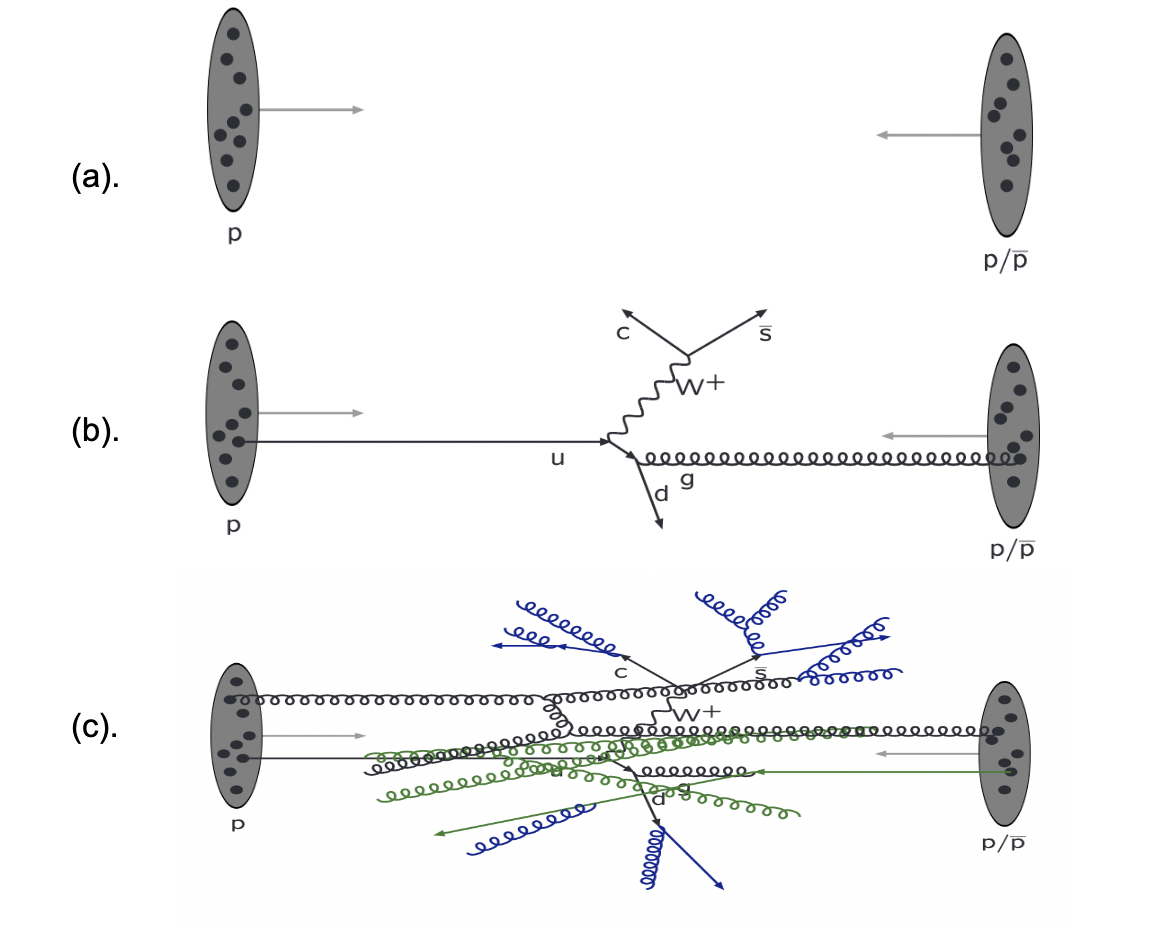
\includegraphics[scale=0.5]{fig/eventStructure.png}
	\label{fig:EventStructure}
\end{figure}


We use two well-known general purpose event generators in this analysis: \SHERPA~\cite{Gleisberg:2008ta} and \PYTHIA8.2~\cite{bierlich2022comprehensive, Sjostrand:2008za}. In both generators, the phase space is split into domains, each having their own technologies. See for example \SHERPA's Event Generator Framework in Figure~\ref{fig:sherpaDivideAndConquer}. These domains include the hard process interaction, the parton shower and the hadronization part. The hard process, which occurs at $\mathcal{O}(1)$ TeV, is represented by the matrix element (ME). At  $\mathcal{O}(1)$ TeV, softer scattering particles emerge from parton-parton interactions, beam remnants and initial and final state radiation. These come from quarks and gluons not participating in the main hard process. They radiate gluons and split into quark-antiquark pairs in a splitting process called fragmentation. Fragmentation is dominated by the emission of soft and collinear radiation until the $\Lambda_{QCD} \approx 1 $GeV scale is reached, and via the strong interaction, these fragments snap back into confinement within hadrons. This process is called Hadronization. These domains taken together comprise a full event picture which are represented schematically in Figure~\ref{fig:EventStructure}.

\begin{figure}[!htbp]
    \caption{This image shows the Sherpa Event Generator Framework with the various elements that are needed to produce simulation, from user inputs, to matrix elements to additional interfaces.}
	\centering
	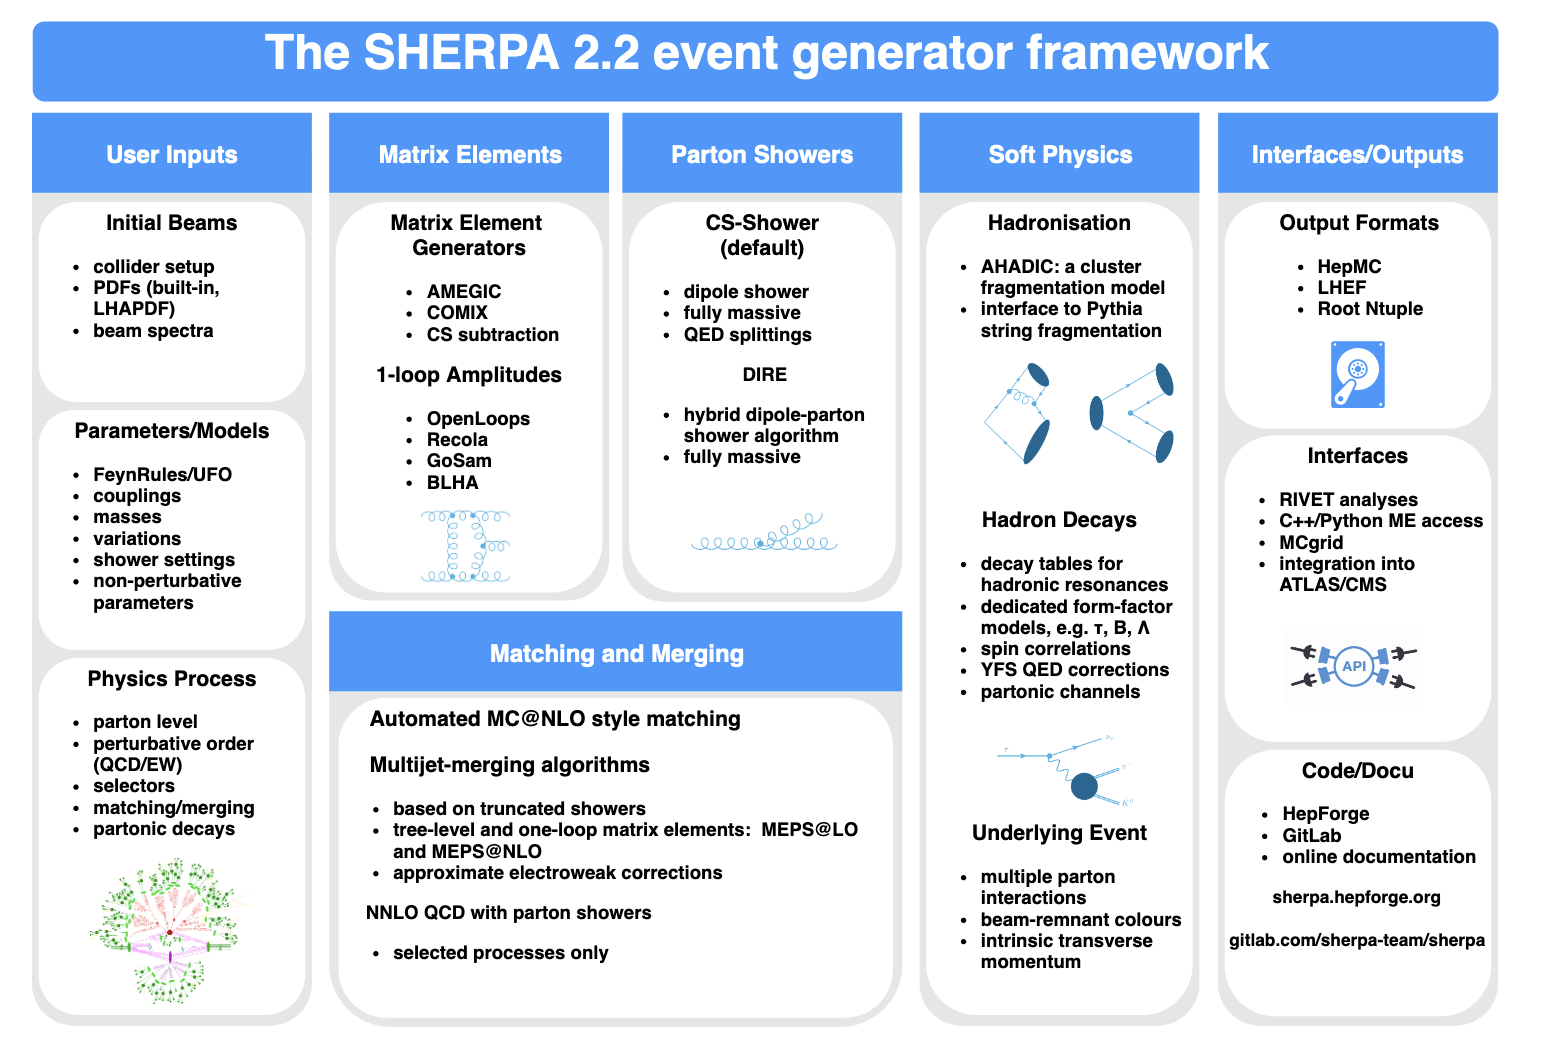
\includegraphics[scale=0.5]{fig/SHERPAD&C.png}
	\label{fig:sherpaDivideAndConquer}
\end{figure}

The Monte Carlo generators also makes use of parton distribution functions (PDFs) which have the descriptions of the probability of some struck parton within the proton to carry a fraction $x$ of the proton's momentum $p$. Both \SHERPA and \PYTHIA8 include the NNPDF~\cite{NNPDF:2021uiq} set of parton distribution functions. NNPDF makes use of neural networks to extract PDFs from data to describe the structure of protons in terms of their quark and gluon constituents. These PDFs cannot be computed from first principles and hence must be extracted from data by carefully matching data with their corresponding theoretical predictions dictated by non-perturbative QCD. The PDFs are also a function of the factorization scale $\mu_{f}$ which roughly separates the long-distance (lower energy) and short-distance (higher energy) processes. This is typically set at $\mu_{f}\approx Q^{2}$, the hard scattering scale where $Q^2$ represents the scale of the collision momentum transfer. At short-distances, QCD is perturbative but for longer-distances non-perturbative techniques are employed. 

% The factorization scale is usually set at the scale of the hard scattering interaction $\mu_{f} \approx Q^{2}$ where $Q^2$ is the momentum transfer in the collision.

\begin{figure}[!htbp]
    \caption{Latest results of the global fit done by the NNPDF collaboration showing the PDFs at factorization scales of 10~$\GeV^{2}$ and 10~$\GeV^{4}$. The different PDFs are related by the DGLAP evolution equations~\cite{DelDebbio:2018siw}}
	\centering
	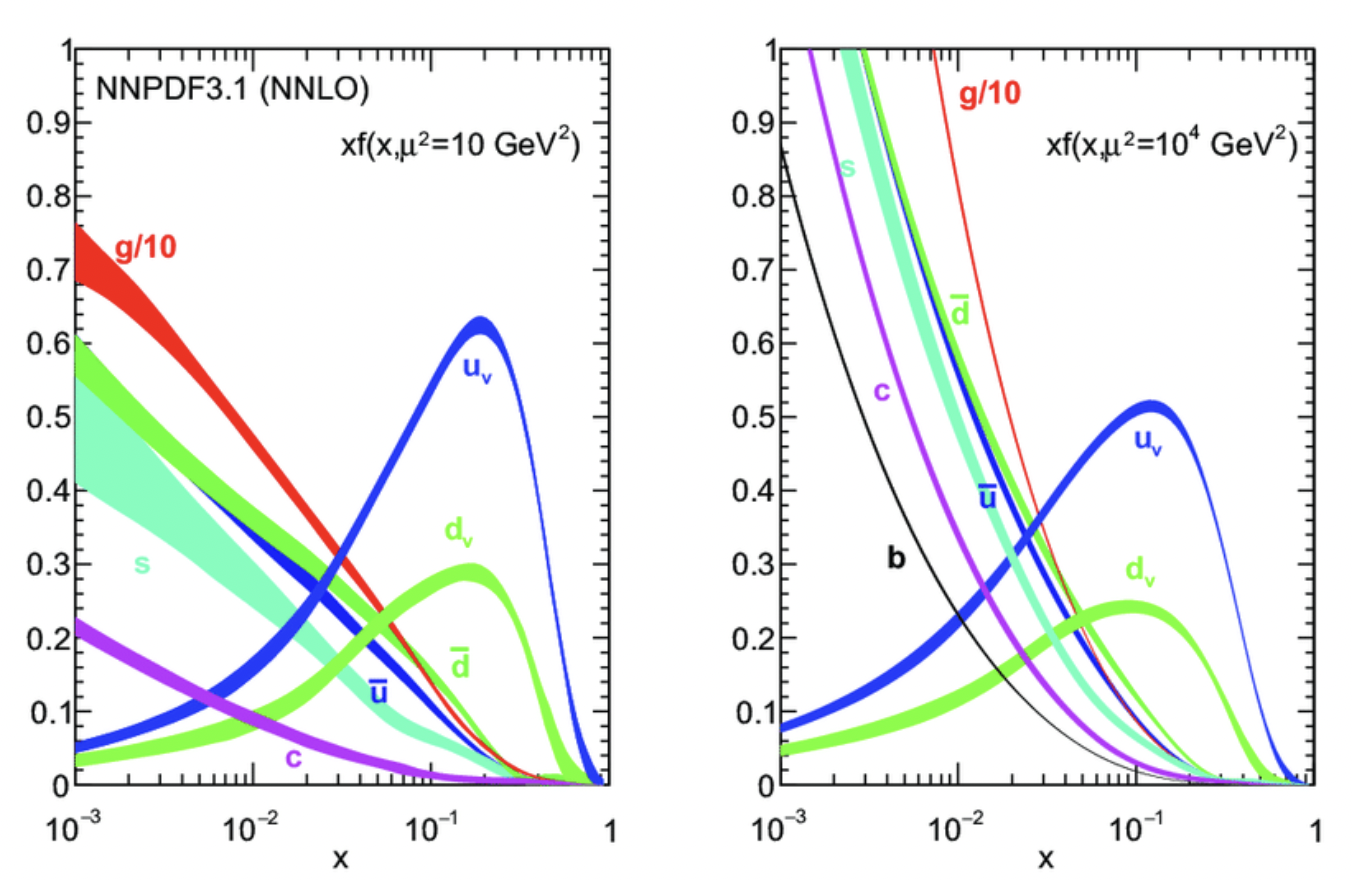
\includegraphics[scale=0.5]{fig/NNPDFGlobalFit.png}
	\label{fig:NNPDF}
\end{figure}

The generators allow users to configure the collider setup, the PDFs, other underlying-event parameters \cite{Sirunyan:2019dfx}, as well as the main physics model and their corresponding decays to a final state. 

% First, the hard scattering process is described by the matrix element (ME) calculators, and then the Parton Showers (PS) regime are an attempt at constructing the entire event. The two regimes are combined via the Matching and Merging (M&M) scheme 

\subsection{Background Determination}

This dissertation searches for non-resonant BSM signatures decaying into the two-photon final state. In this analysis, we account for two main sources of background, 1.) Real background: SM Prompt Diphoton, 2.) Fake Background, which comes from jets that fragment and are misidentified as photons in the detector. The SM diphoton real background is the dominant, irreducible background which is determined up to next-to-next-to-leading (NNLO) accuracy. The subdominant background coming from ``fakes" is on the other hand, reducible and is estimated from control samples in data. 


% \begin{tikzpicture}
%   \begin{feynman}
%     \vertex (a);
%     \vertex [right=of a] (b);
%     \vertex [below=of b] (c);
%     \vertex [left=of c] (d);
%     \vertex [right=of b] (p1);
%     \vertex [right=of c] (p2);

%     \diagram* {
%       (a) -- [fermion] (b) -- [fermion] (c),
%       (c) -- [fermion] (d),
%       (b) -- [photon] (p1), 
%       (c) -- [photon] (p2)
%     };
%   \end{feynman}
% \end{tikzpicture}

%%%%% BOX DIAGRAM
% \begin{tikzpicture}
%   \begin{feynman}
%     \vertex (a);
%     \vertex [right=of a] (b);
%     \vertex [right=of b] (c);
%     \vertex [below=of b] (d);
%     \vertex [below=of c] (f);
%     \vertex [left=of f] (d);
%     \vertex [left=of d] (e);
%     \vertex [right=of c] (p1);
%     \vertex [right=of f] (p2);

%     \diagram* {
%       (a) -- [gluon] (b) -- [fermion] (c),
%       (b) -- [fermion] (d),
%       (d) -- [gluon] (e),
%       (c) -- [fermion] (f),
%       (f) -- [fermion] (d),
%       (c) -- [photon] (p1), 
%       (f) -- [photon] (p2)
%     };
%   \end{feynman}
% \end{tikzpicture}

\section{Nonresonant Prompt Diphoton Background}\label{sec:bkg_real}
The main source of the background arises from the prompt SM diphoton production, $pp\longrightarrow \gamma\gamma$, which occurs via quark annihilation (``Born'') or the gluon fusion process (``Box''). These are illustrated in Figure~\ref{fig:LOFeynmanBackgroundDiphoton}. The Born process dominates over the box process due to large quark PDFs. These processes constitute the irreducible background for this search. We use the \SHERPA event-generator to prepare diphoton+jets (GGJets) Monte Carlo sample which include the effects of detector simulation. 

\begin{figure}[!htbp]
\caption{The irreducible and primary background for the analysis comes from the prompt standard model $\gamma\gamma$ production which occur via the q-q$\Bar{q}$ annihilation (Born) or through the gluon fusion (Box)  process as shown from left to right.}
\begin{center}
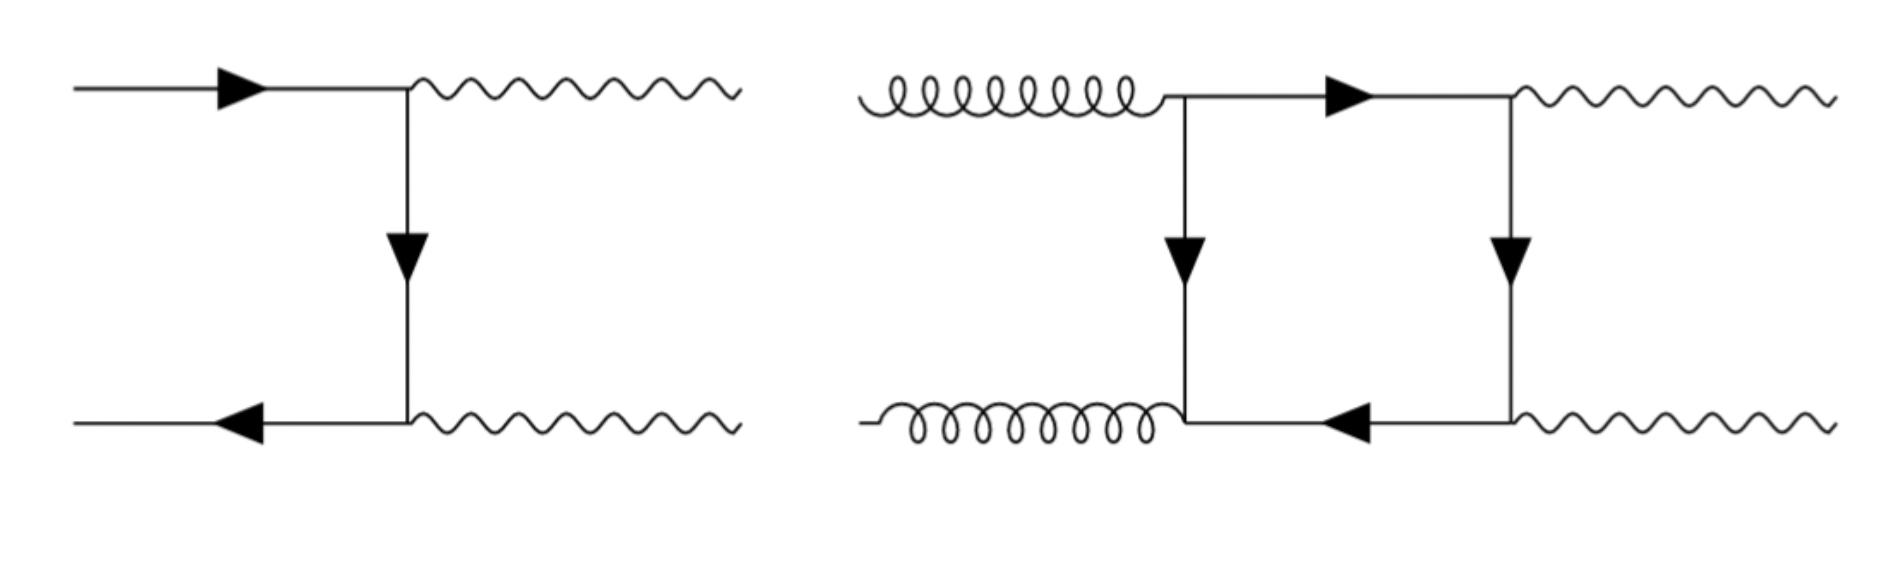
\includegraphics[angle=0,width=0.7\textwidth]{fig/PromptDiphotonBackground.png}
\end{center}
\label{fig:LOFeynmanBackgroundDiphoton}
\end{figure}


\begin{figure}[htbp!]
\caption{Sample Feynman Diagrams for (a) $q\Bar{q}$ and (b) gq-initiated processes for NLO SM diphoton production are shown. \cite{DErrico:2011cgc}}
\begin{center}
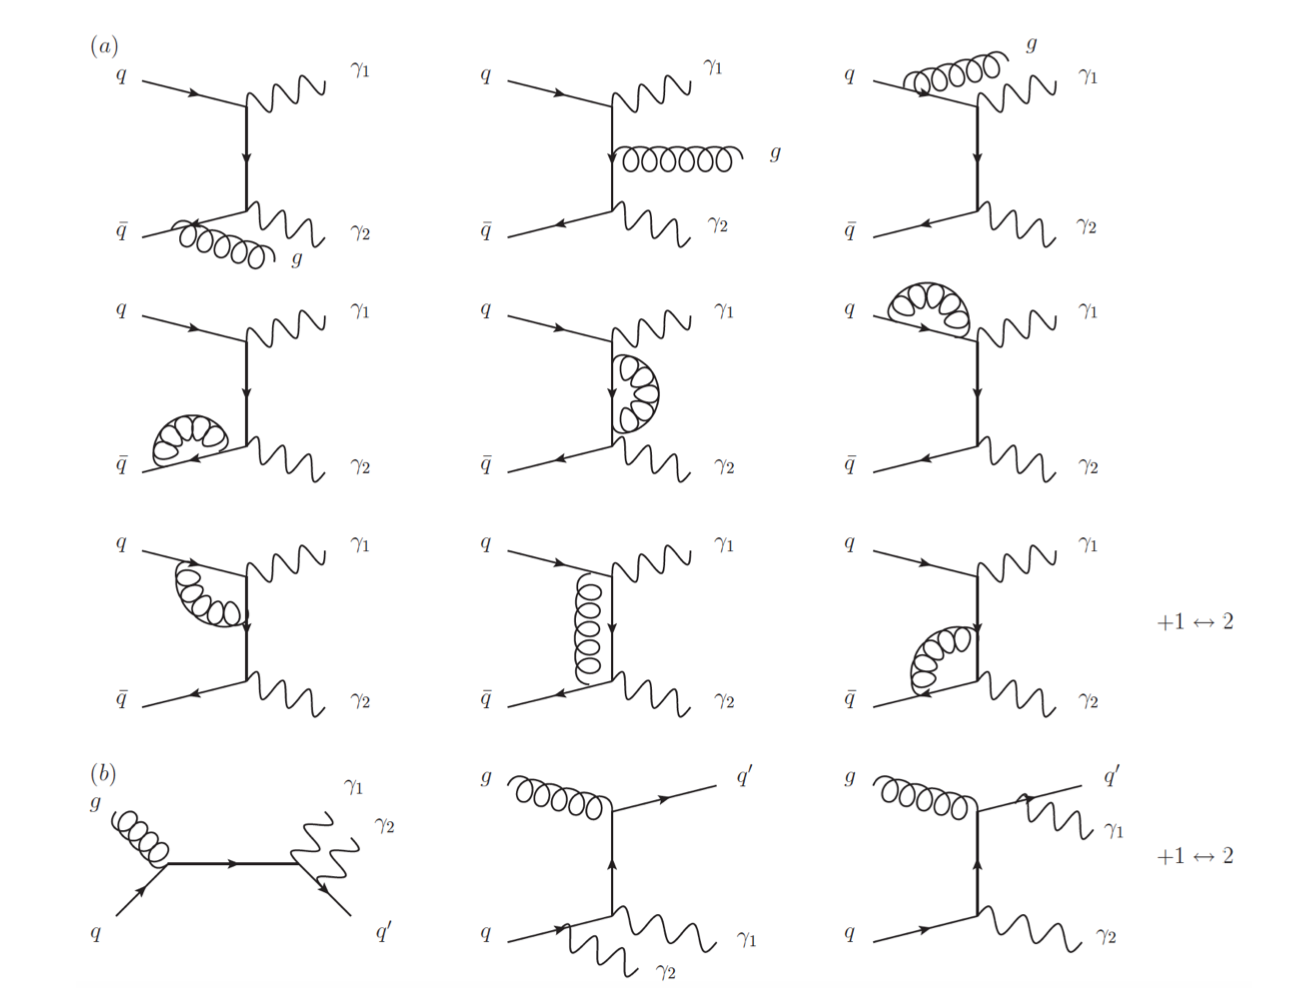
\includegraphics[angle=0,width=0.7\textwidth]{fig/FeynmanDiagramsNLO.png}
\end{center}
\label{fig:NLOSMBackground}
\end{figure}

Additionally, up to three additional final state partons, i.e. ($\gamma\gamma + nj$) are included in \SHERPA. Here, $j$ stands for jets and $n$ stands for $n = 0, 1, 2, 3$. While gq-initiated processes are also possible, it is formally a higher-order term and is suppressed compared to the box process due to the same reason. These contributions arise at NLO are not present at LO and scale variations of the quark-antiquark contributions that are present at LO do not provide a reliable estimate of these contributions. Similarly, the gluon-gluon-initiated contributions in the box diagram at NNLO are absent at LO. 


% The Born process includes up to three additional final state partons, i.e. $pp\longrightarrow \gamma\gamma + nj$ where $j$ stands for jet and $n = 0,$ 1, 2, or 3. The Box process on the other hand, is formally at NNLO however its contribution to the overall cross-section or the diphoton production rate is comparable to the leading order contribution due to the large quark PDFs. 

% The NLO and NNLO predictions do not lie within the scale variations at LO and NLO, re-505
% spectively. Quark-gluon-initiated contributions that arise at NLO are not present at LO and so506
% scale variations of the quark-antiquark contributions that are present at LO do not provide a507
% reliable estimate of these contributions. Similarly, the gluon-gluon-initiated contributions that508
% contribute via a box diagram at NNLO are absent at LO. However, the SHERPA + 3 jet MC509
% includes the quark-gluon contributions involving real radiation that arise at NLO.

It must be noted that \SHERPA only includes the real radiation component of these higher order processes. The virtual corrections will later on be accounted in the K-factor corrections calculated from \MCFM which will be discussed in more detail in the next section. A distinguishing trait of calculators versus event generators is that, the former's output cannot be interfaced with a program such as \GEANT4 which accounts for detector effects on the outgoing particles in a collision. However, they can calculate the diphoton cross-section at generator-level in a specified phase space and yield various kinematic distributions.

Higher order corrections have been shown to substantially reduce scale uncertainties estimated from scale variations on total cross section predictions \cite{Badger:2013ava}. Additional final state jets are important in sampling the diphoton phase space as shown in Ref.~\cite{CMS-PAS-EXO-12-045}. It was found that the separation in $\phi$ of the two photons are sensitive to the presence of the additional jets and using an leading-order LO simulation was insufficient for calculating the process. \SHERPA applies event weights to the additional final state partons. These weights are accounted for in the analysis. Final state photons could also come from non-perturbative contributions, i.e. fragmentations from a quark or gluon, where soft or collinear photons are emitted from harder jets through a QED $q\longrightarrow q\gamma$ splittings. \SHERPA interlaces photons into the QCD + QED parton shower. This fragmentation is represented in Figure~\ref{fig:NLOSMBackgroundFragmentation}


\begin{figure}[htbp!]
\caption{Representative Feynman Diagrams for NLO diphoton production through quark or gluon fragmentation \cite{DErrico:2011cgc}}
\begin{center}
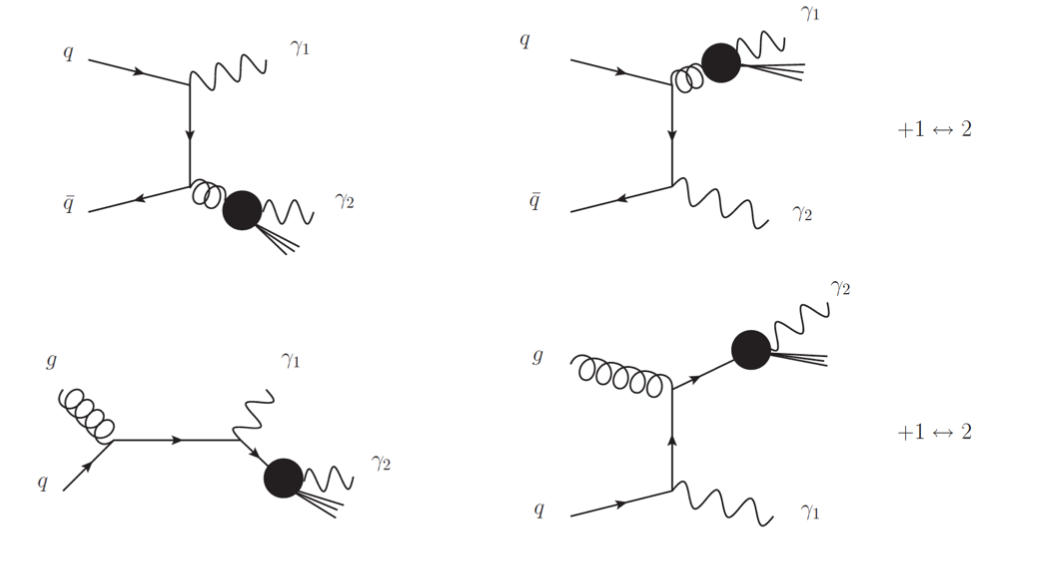
\includegraphics[angle=0,width=0.7\textwidth]{fig/GluonOrQuarkFragmentation.png}
\end{center}
\label{fig:NLOSMBackgroundFragmentation}
\end{figure}

\subsubsection{The K factor}

As mentioned earlier, our background determination from \SHERPA which has up to 3 final state jets in the simulated events includes most of the QCD real emission component of the higher order corrections to the basic diphoton process. However, virtual corrections are not included. To attempt to remedy this, we use \MCFM v8.0 \cite{Campbell:2016yrh} which is capable of performing a full next-to-next-to-leading order (NNLO) calculation. The MCFM diphoton calculation is based on the $Q_T$-subtraction procedure using N-jettiness as a phase-space-slicing variable~\cite{Campbell:2019dru} and it also includes virtual processes. \MCFM and \SHERPA outputs generator-level distributions which are distributions that are not interfaced with a detector-level simulator like Geant4. An attempt to provide a full NNLO diphoton background prediction is done by calculating the K factor which is the ratio of the \MCFM and \SHERPA outputs. Reweighting the \SHERPA out-of-the-box background prediction with the K-factor accounts for the missing higher order terms and virtual corrections. The K-factor is specifically calculated as a function of the diphoton invariant mass from the ratio of the MCFM NNLO prediction to the \SHERPA MC. The K-factor-reweighted \SHERPA MC events that passed through detector simulation becomes the final prediction for the real SM diphoton invariant mass spectrum. This is shown in Figure~\ref{fig:SMBackgroundKfactorreweighted}.

To avoid bias, K-factor is calculated separately for the diphoton barrel-barrel (BB) and barrel-endcap (BE) acceptance categories. The NNLO cross-section from MCFM is calculated separately in four bins of $m_{\gamma\gamma}}$:

\begin{itemize}
\item $500 < \mgg < 750$\GeV
\item $750 < \mgg < 1000$\GeV
\item $1000 < \mgg < 1500$\GeV
\item $1500 < \mgg < 4000$\GeV
\end{itemize}

If the invariant mass range is too large, larger invariant mass bins within the range wouldn't be adequately sampled. This is because the stopping criteria for the estimated accuracy of the numerical integration will be satisfied early. These separate bins, weighted by their cross-sections are ultimately stitched together to form a continuous and smooth distribution. 

\begin{figure}[htbp!]
\caption{Shown here are the out-of-the-box SHERPA prompt simulated \mgg prediction reweighted with the K-factor in light teal. The fake prediction is shown with a darker shade of teal.}
\begin{center}
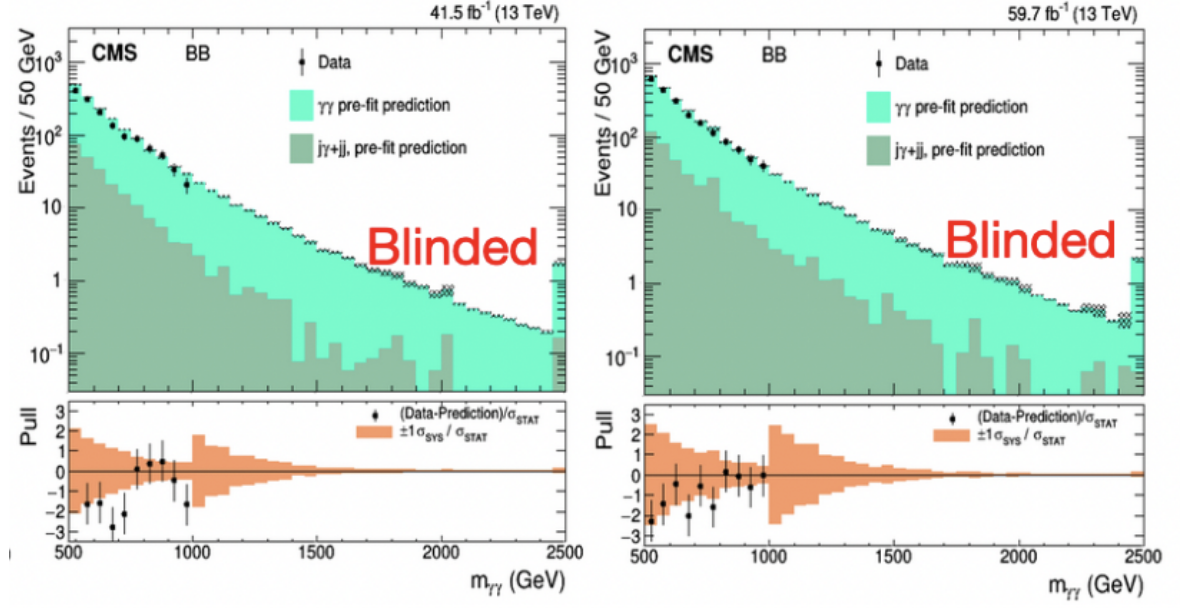
\includegraphics[angle=0,width=0.9\textwidth]{fig/diphotonblinded.png}
\end{center}
\label{fig:SMBackgroundKfactorreweighted}
\end{figure}

Figure~\ref{fig:kfactor_mgg}, shows the K factor distributions for both barrel-barrel and barrel-endcap diphotons. The effects of simultaneously varying the renormalization $\mu_{r}$ and factorization $\mu_{f}$ scales by a factor of two in each direction, up and down around the nominal prediction which is the diphoton invariant mass. The parameters, $\mu_{r}$ and $\mu_{f}$ are introduced in QCD calculations to remedy the UV and infrared divergences in the calculation of the amplitude squared of any given partonic process. The UV divergences come from large momentum in the loops of Feynman diagrams while infrared divergences happen due to virtual or real particle that reach zero momentum. The coupling constant $\alpha_{s}$ becomes a function of the renormalization scale $\mu_{r}$. The PDF, introduced earlier in the chapter, and fragmentation functions will become a function of the factorization scale. The choice of varying the scale factors as done here is often sufficient to know how observables vary within those scales.

% \footnote{UV divergences appear because of large momentum in the loops of Feynman diagrams representing the amplitude while infrared divergences appear when either a virtual or real particle can reach a zero momentum \FIXME{citation: https://physics.stackexchange.com/questions/365124/what-is-meant-by-factorization-scale-factor-in-qcd-calculations}} 


% generated by Tools/bin/plotKFactor.cc
\begin{figure}[htbp!]
\caption{NNLO k-factor for the $m_{\gamma\gamma}$ distribution for barrel-barrel
  diphotons (left) and barrel-endcap diphotons (right) for the real diphoton k-factor. The
  renormalization $\mu_{r}$ and factorization $\mu_{f}$ scales have been varied as follows: $\mu_{r}=\mu_{f}=$ 0.5$m_{\gamma\gamma}$ (top), 1.0$m_{\gamma\gamma}$ (middle), and 2.0$m_{\gamma\gamma}$(bottom). The cuts on the generator-level photons are the same as the kinematic cuts used offline.}
\begin{center}
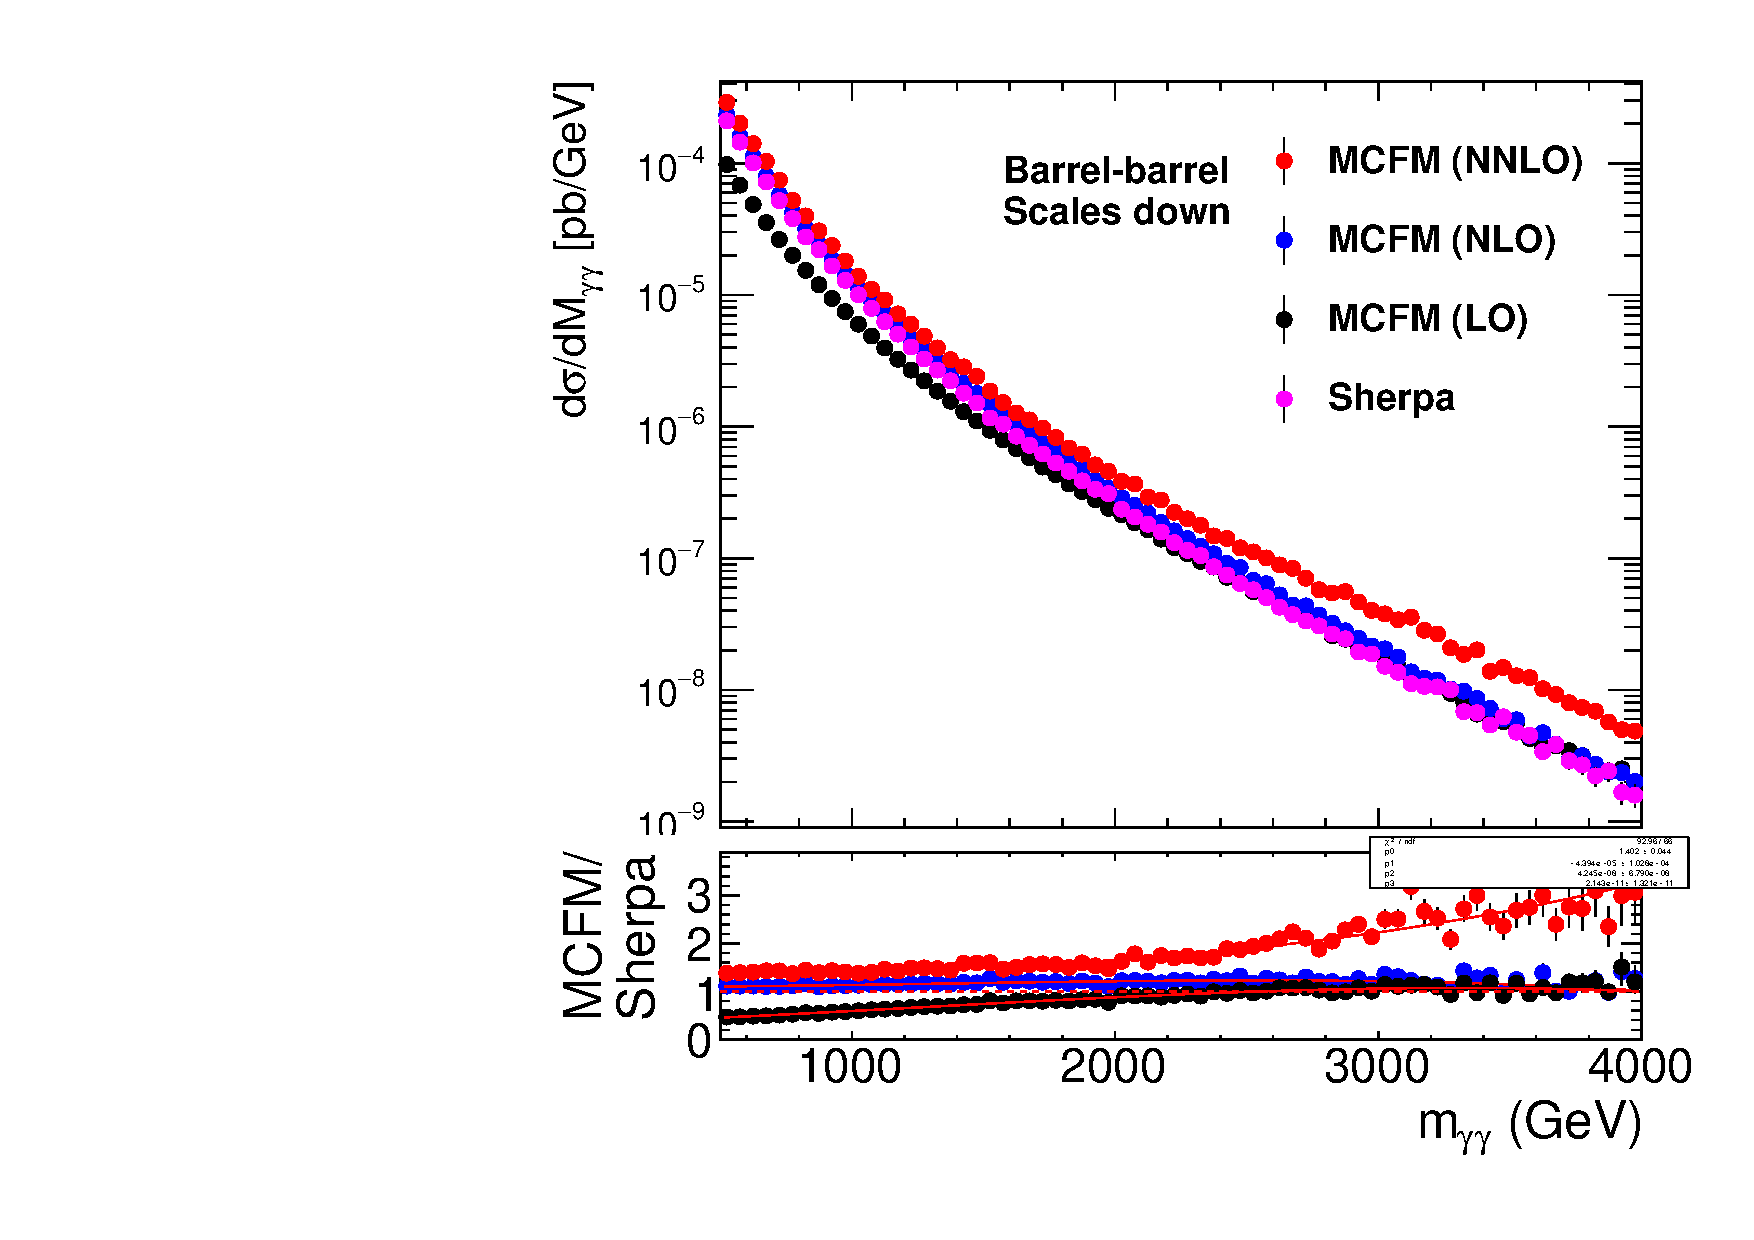
\includegraphics[angle=0,width=0.33\textwidth]{fig/BB_hist1_R0p5F0p5_125GeV_NNPDF.pdf}
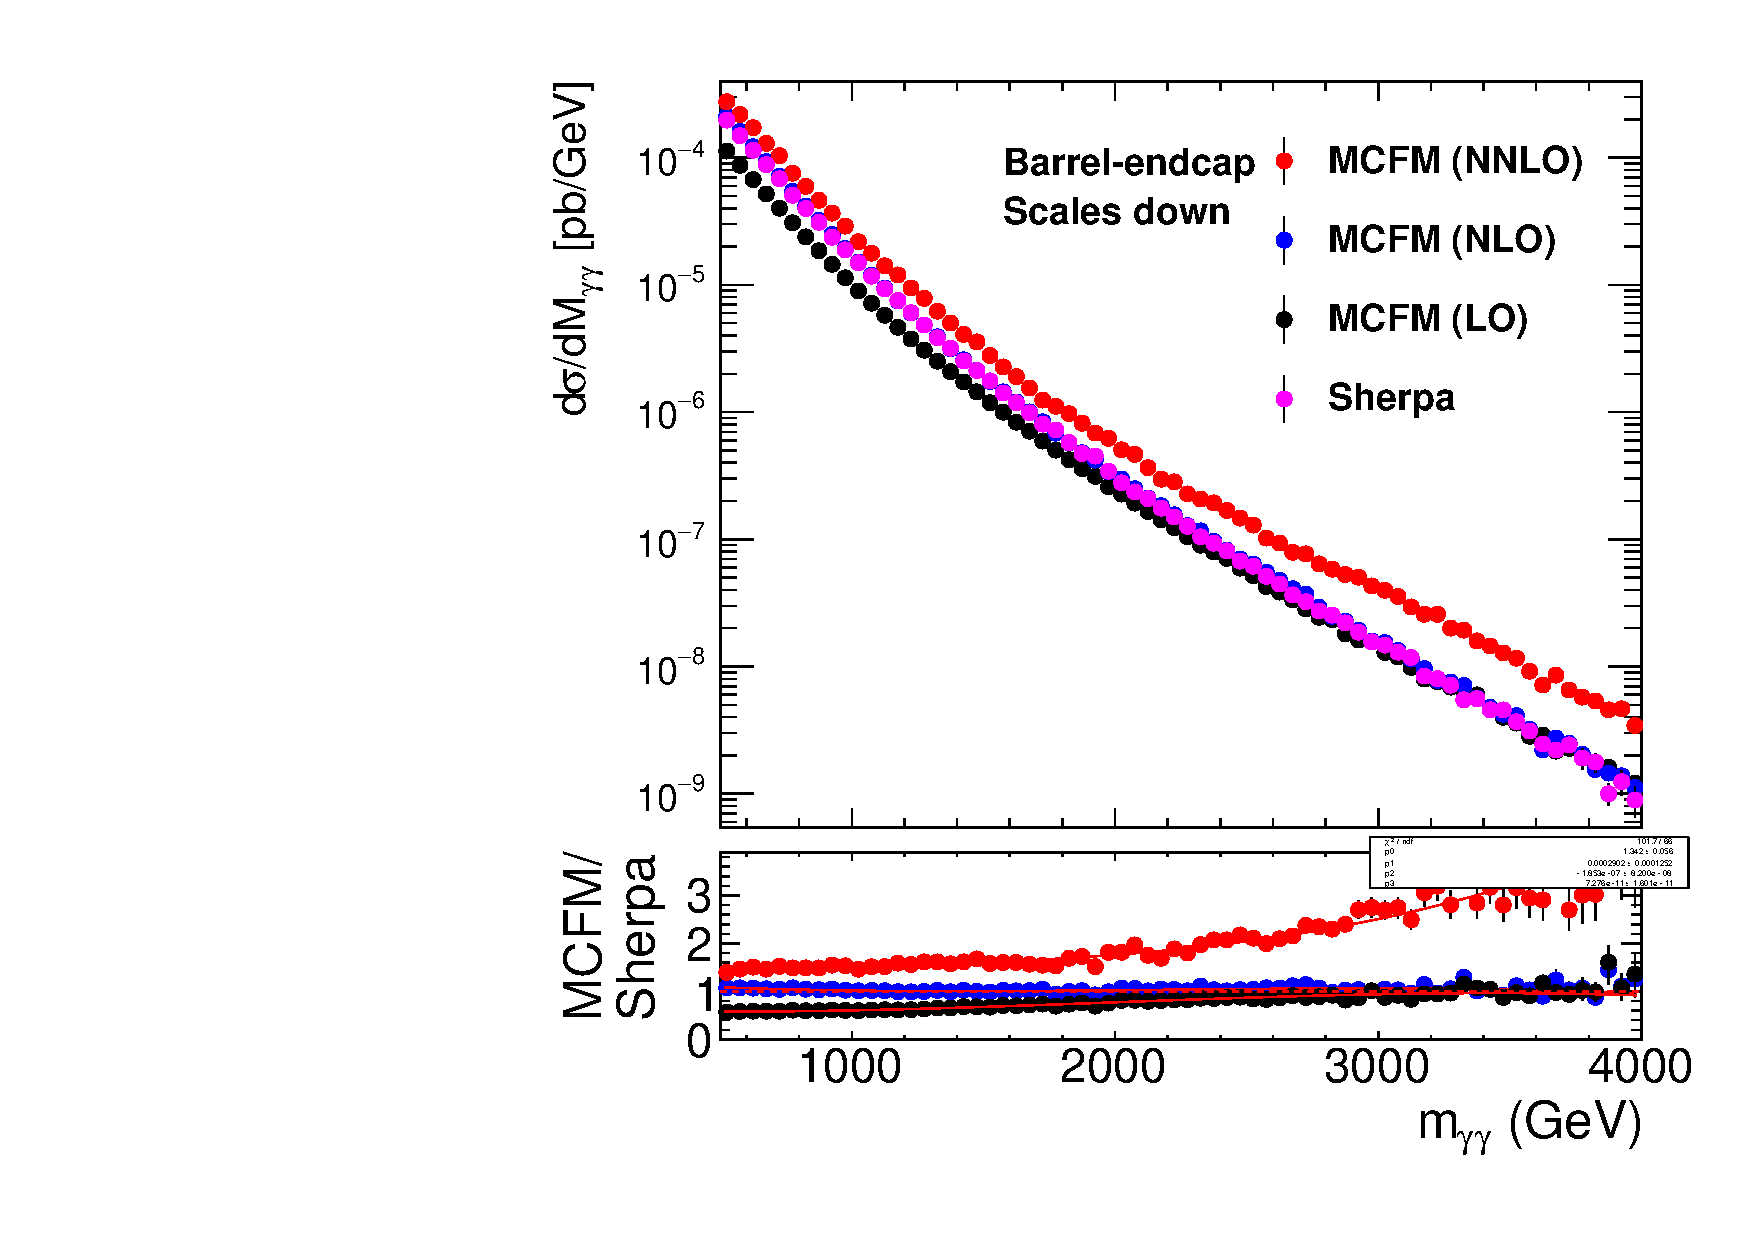
\includegraphics[angle=0,width=0.33\textwidth]{fig/BE_hist1_R0p5F0p5_125GeV_NNPDF.pdf}
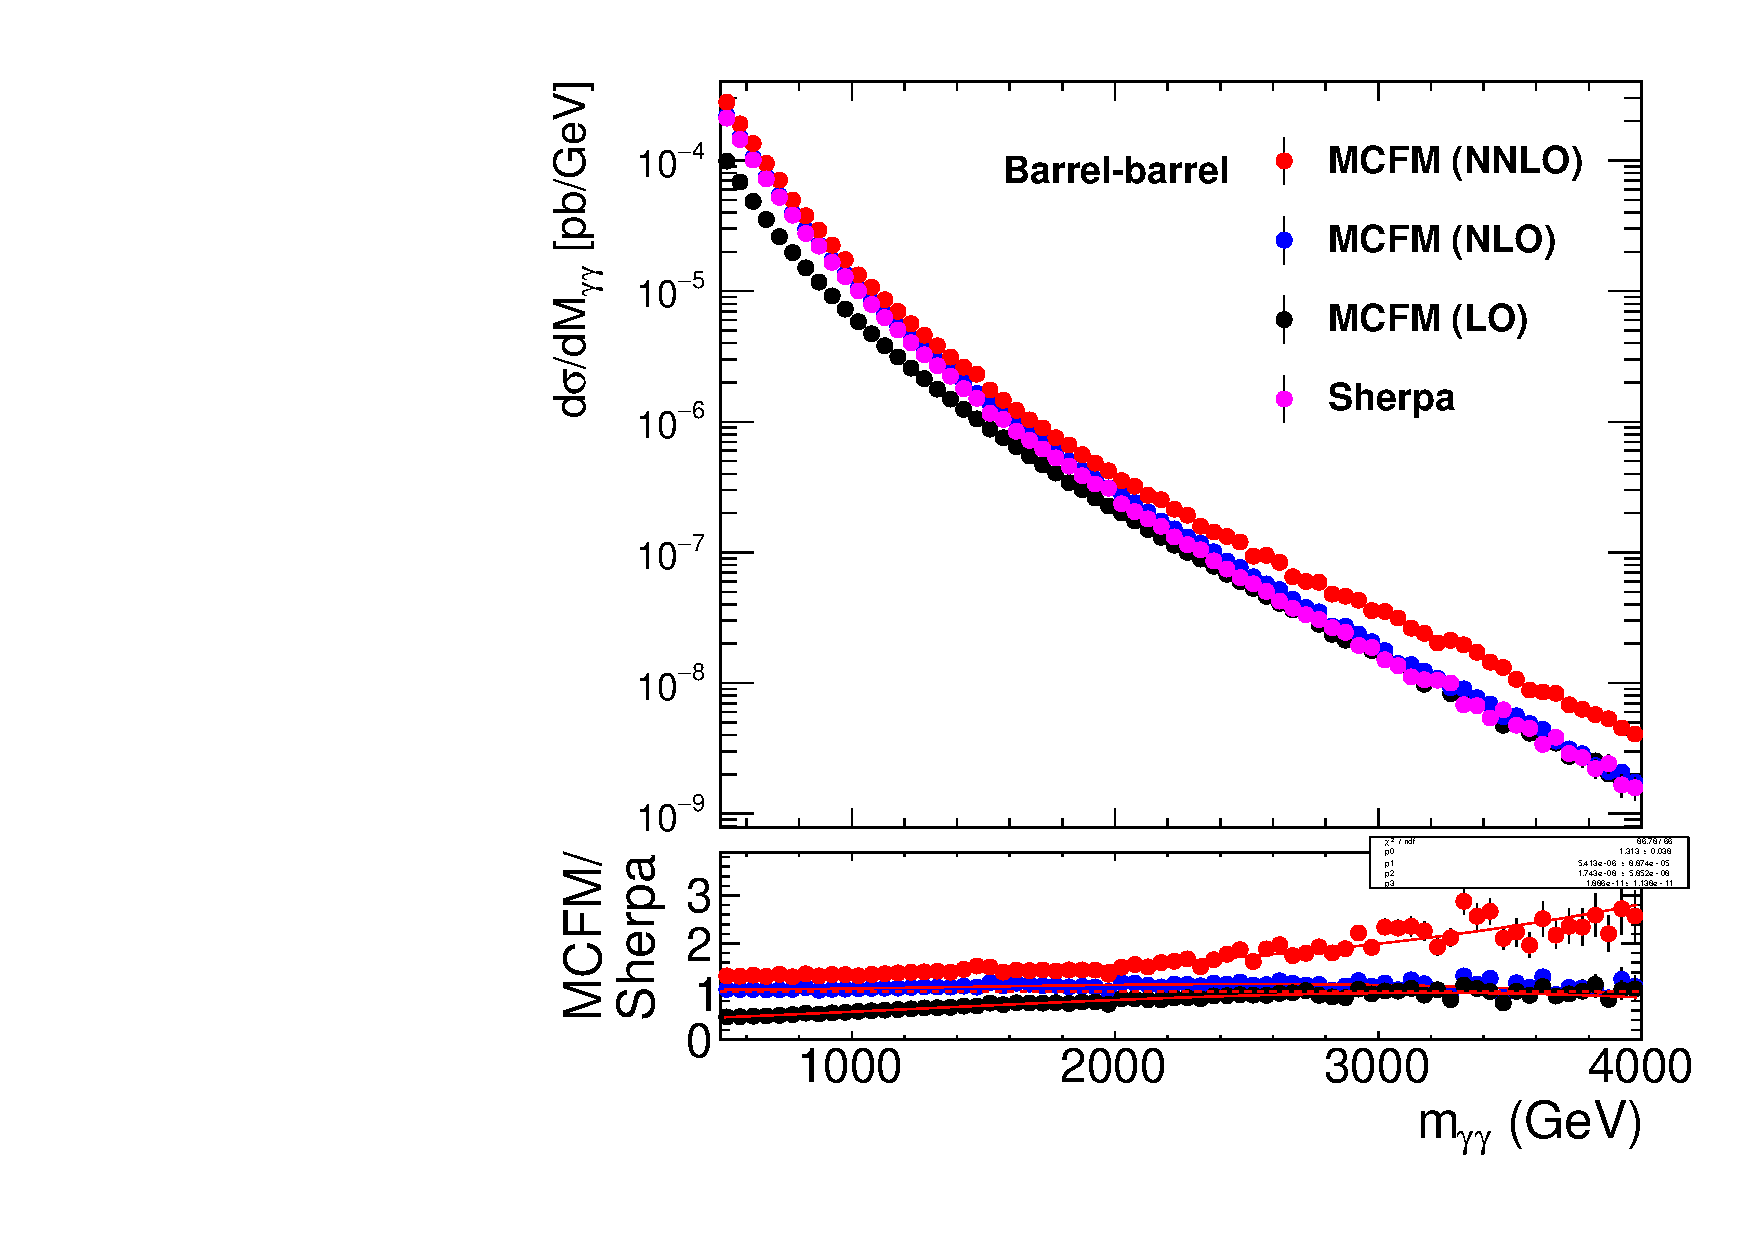
\includegraphics[angle=0,width=0.33\textwidth]{fig/BB_hist1_R1F1_125GeV_NNPDF.pdf}
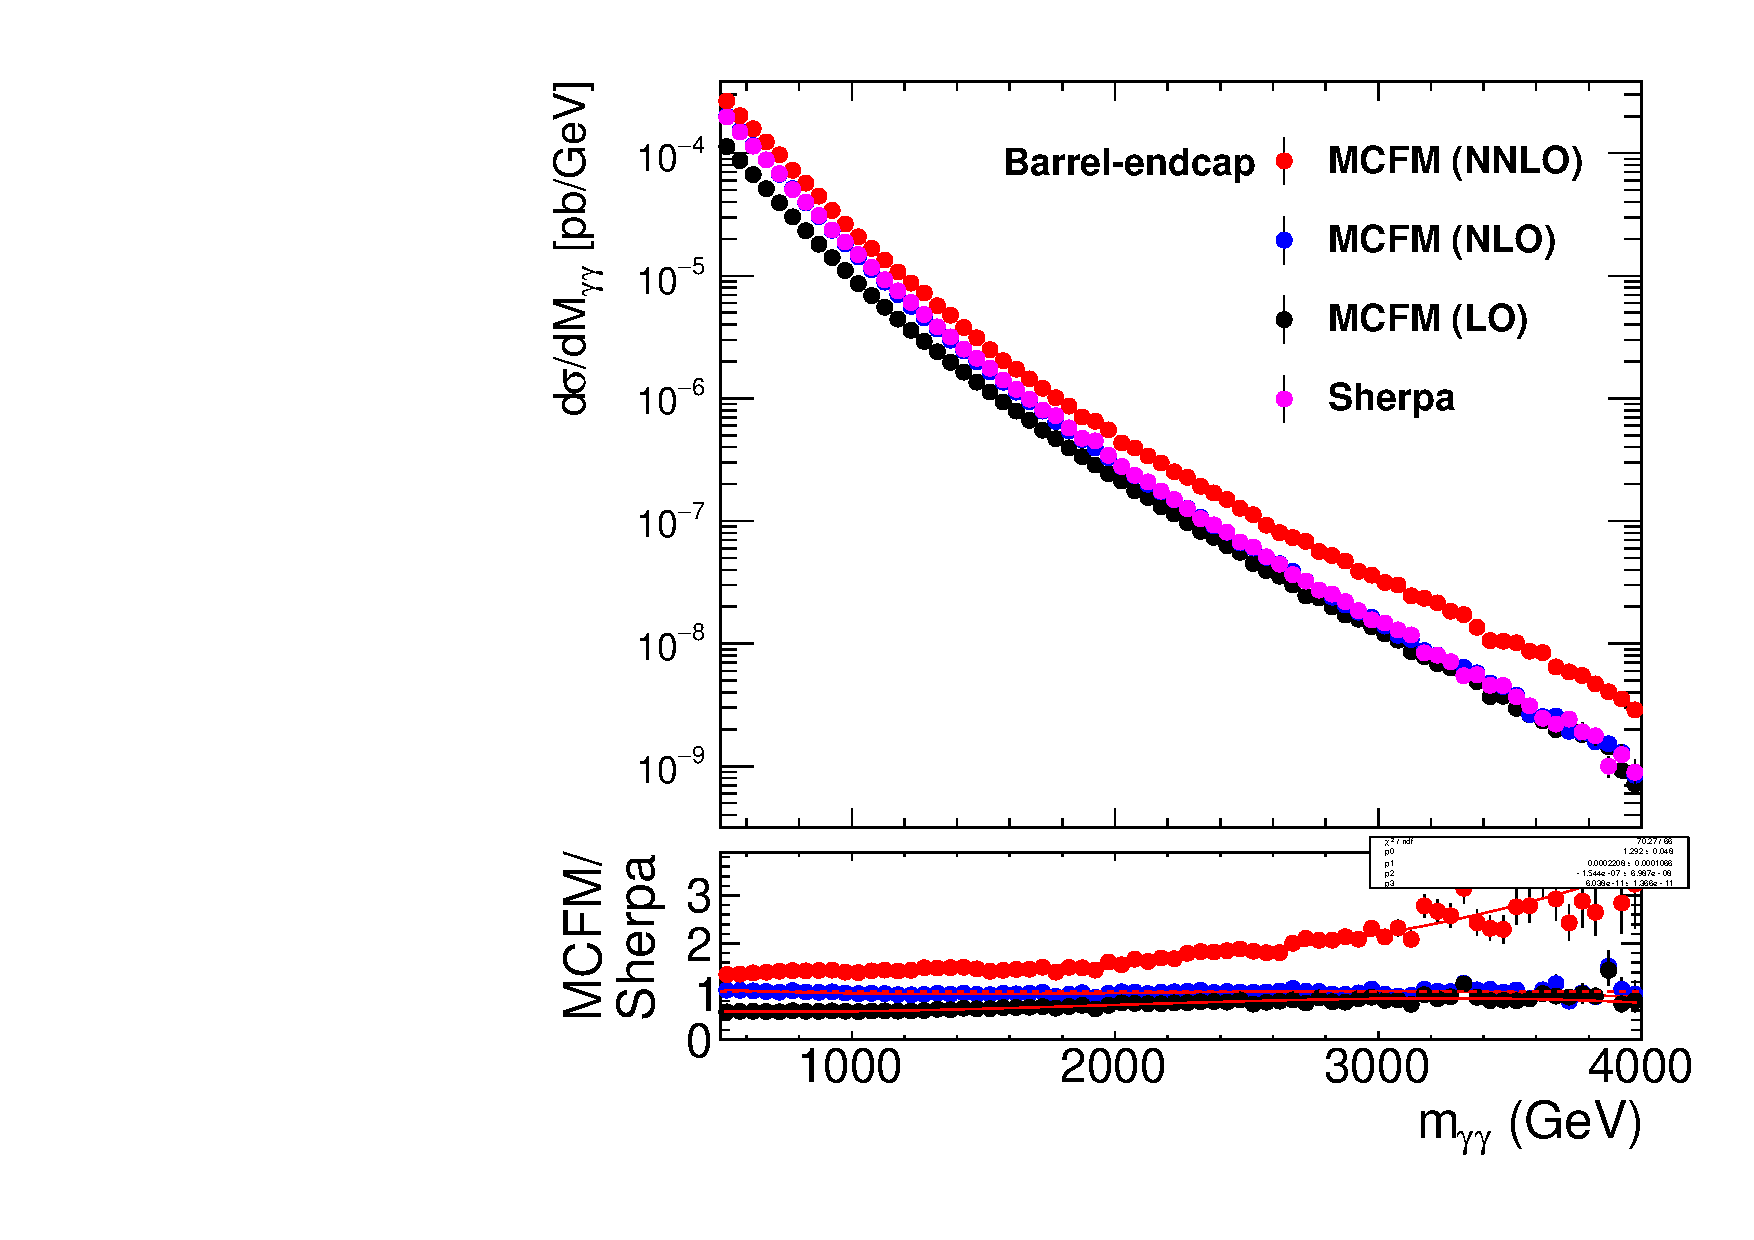
\includegraphics[angle=0,width=0.33\textwidth]{fig/BE_hist1_R1F1_125GeV_NNPDF.pdf}
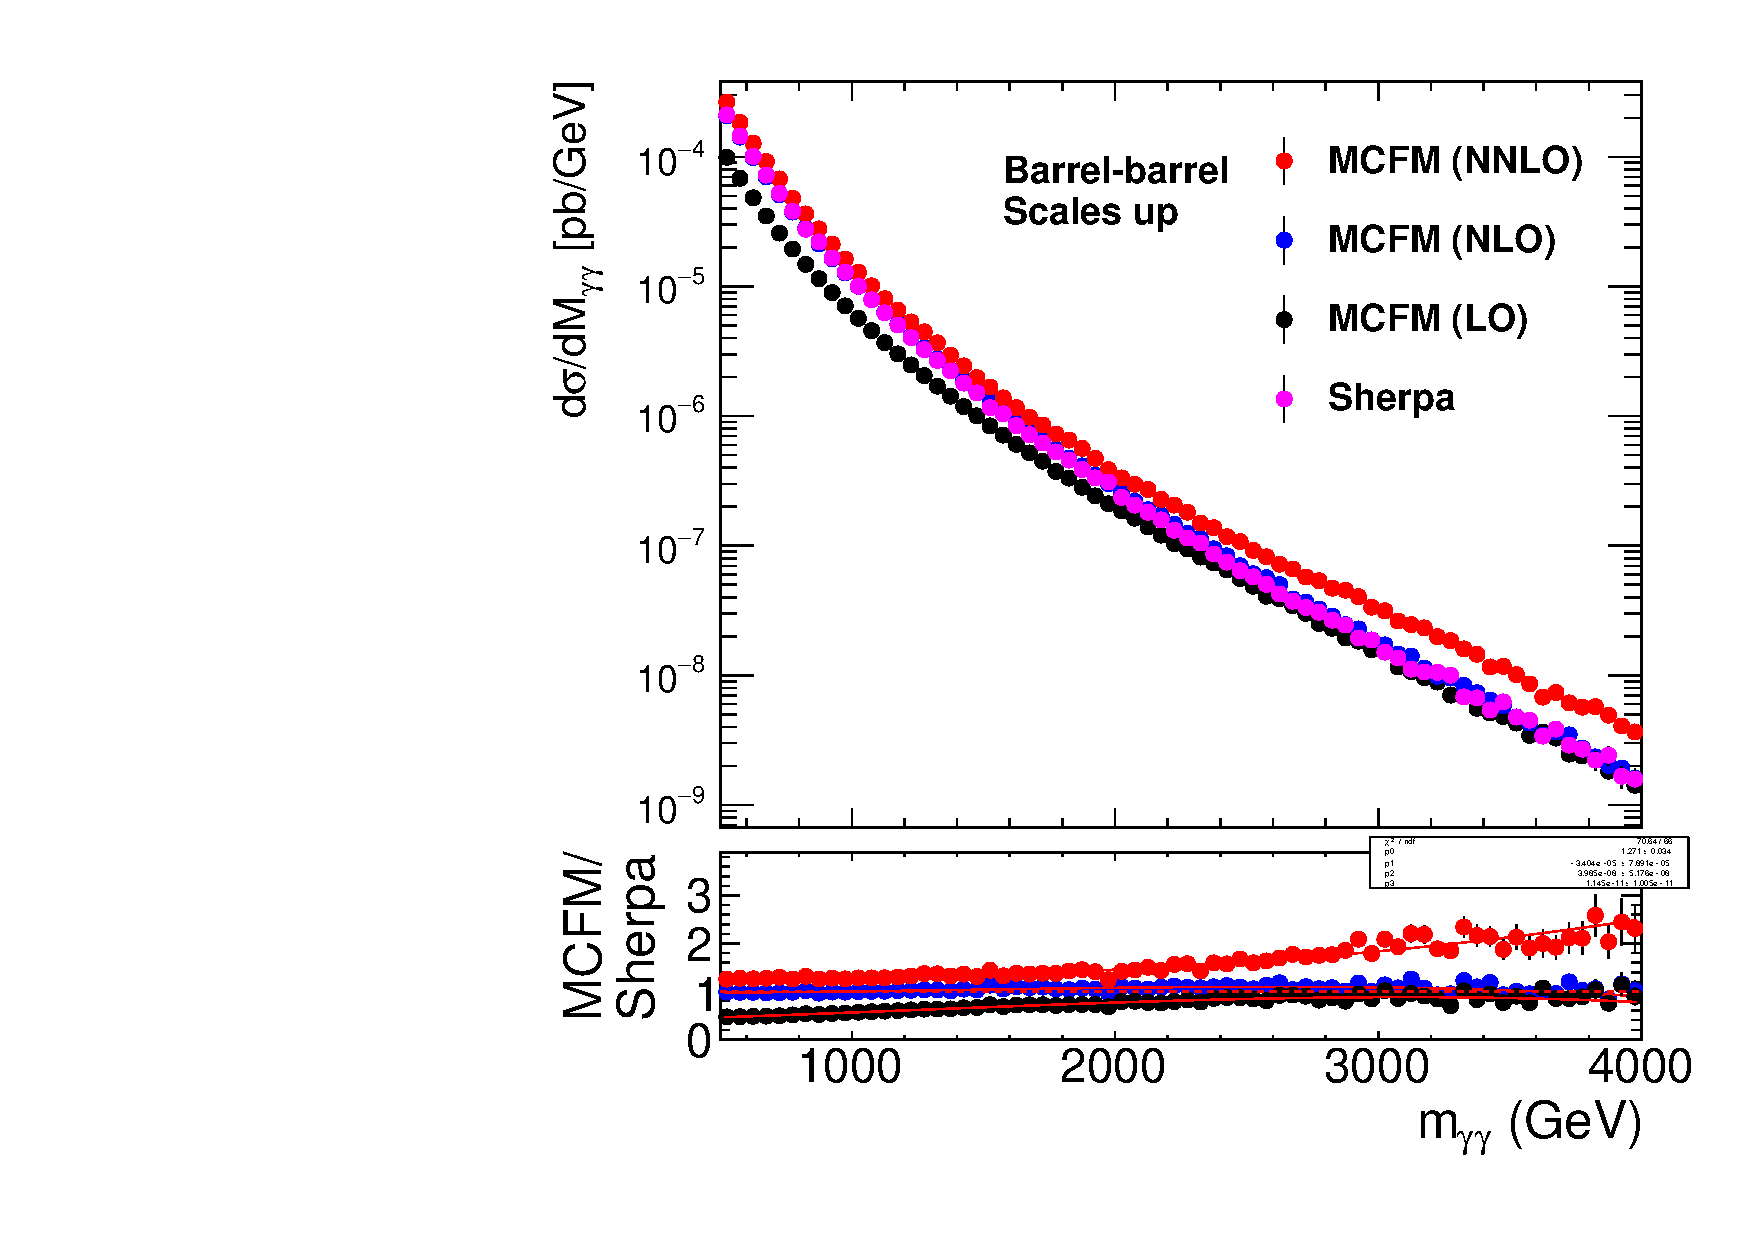
\includegraphics[angle=0,width=0.33\textwidth]{fig/BB_hist1_R2F2_125GeV_NNPDF.pdf}
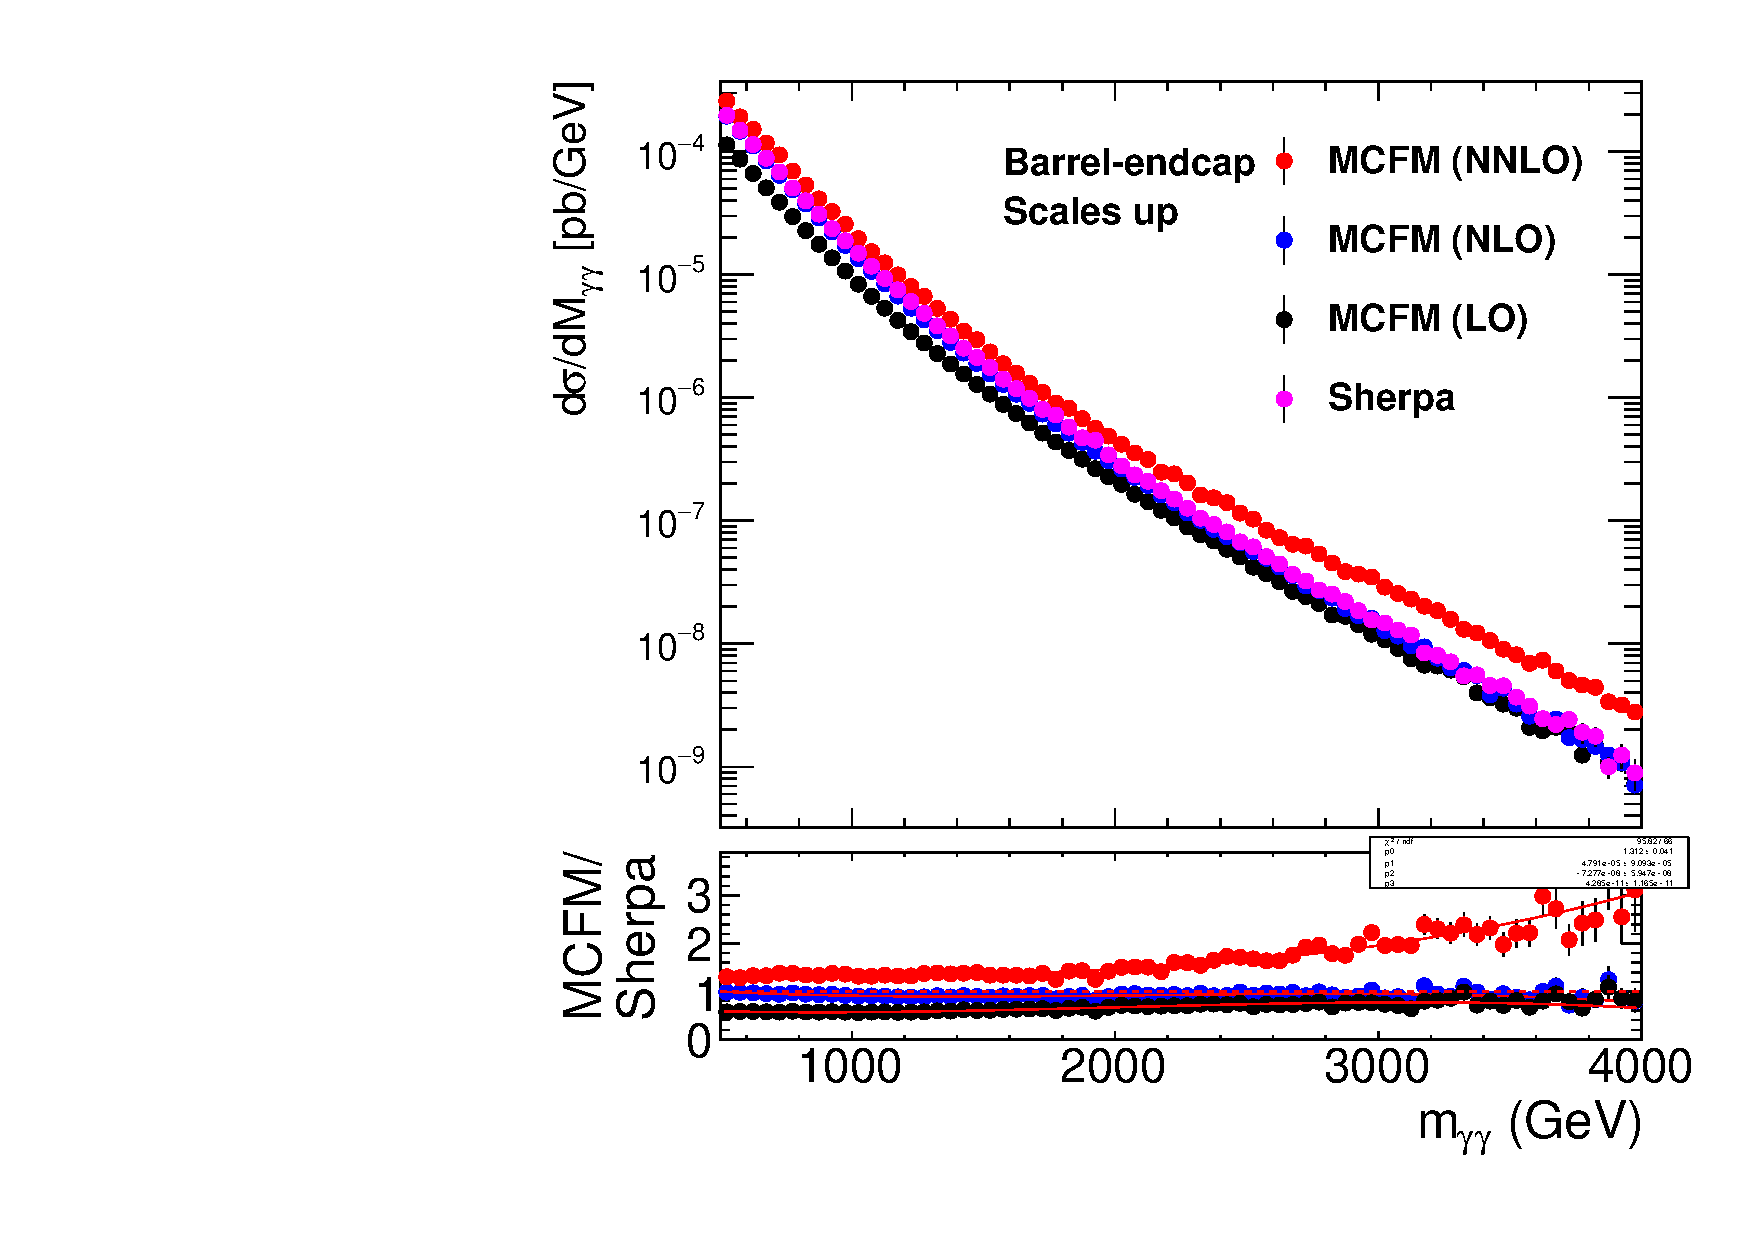
\includegraphics[angle=0,width=0.33\textwidth]{fig/BE_hist1_R2F2_125GeV_NNPDF.pdf}
\end{center}
\label{fig:kfactor_mgg}
\end{figure}

% generated by Tools/bin/draw_kfactor.cc
\begin{figure}[htbp!]
\caption{Ratio of diphoton cross sections calculated by MCFM versus the results from \SHERPA in the barrel-barrel (left) and barrel-endcap (right) regions.}
\begin{center}
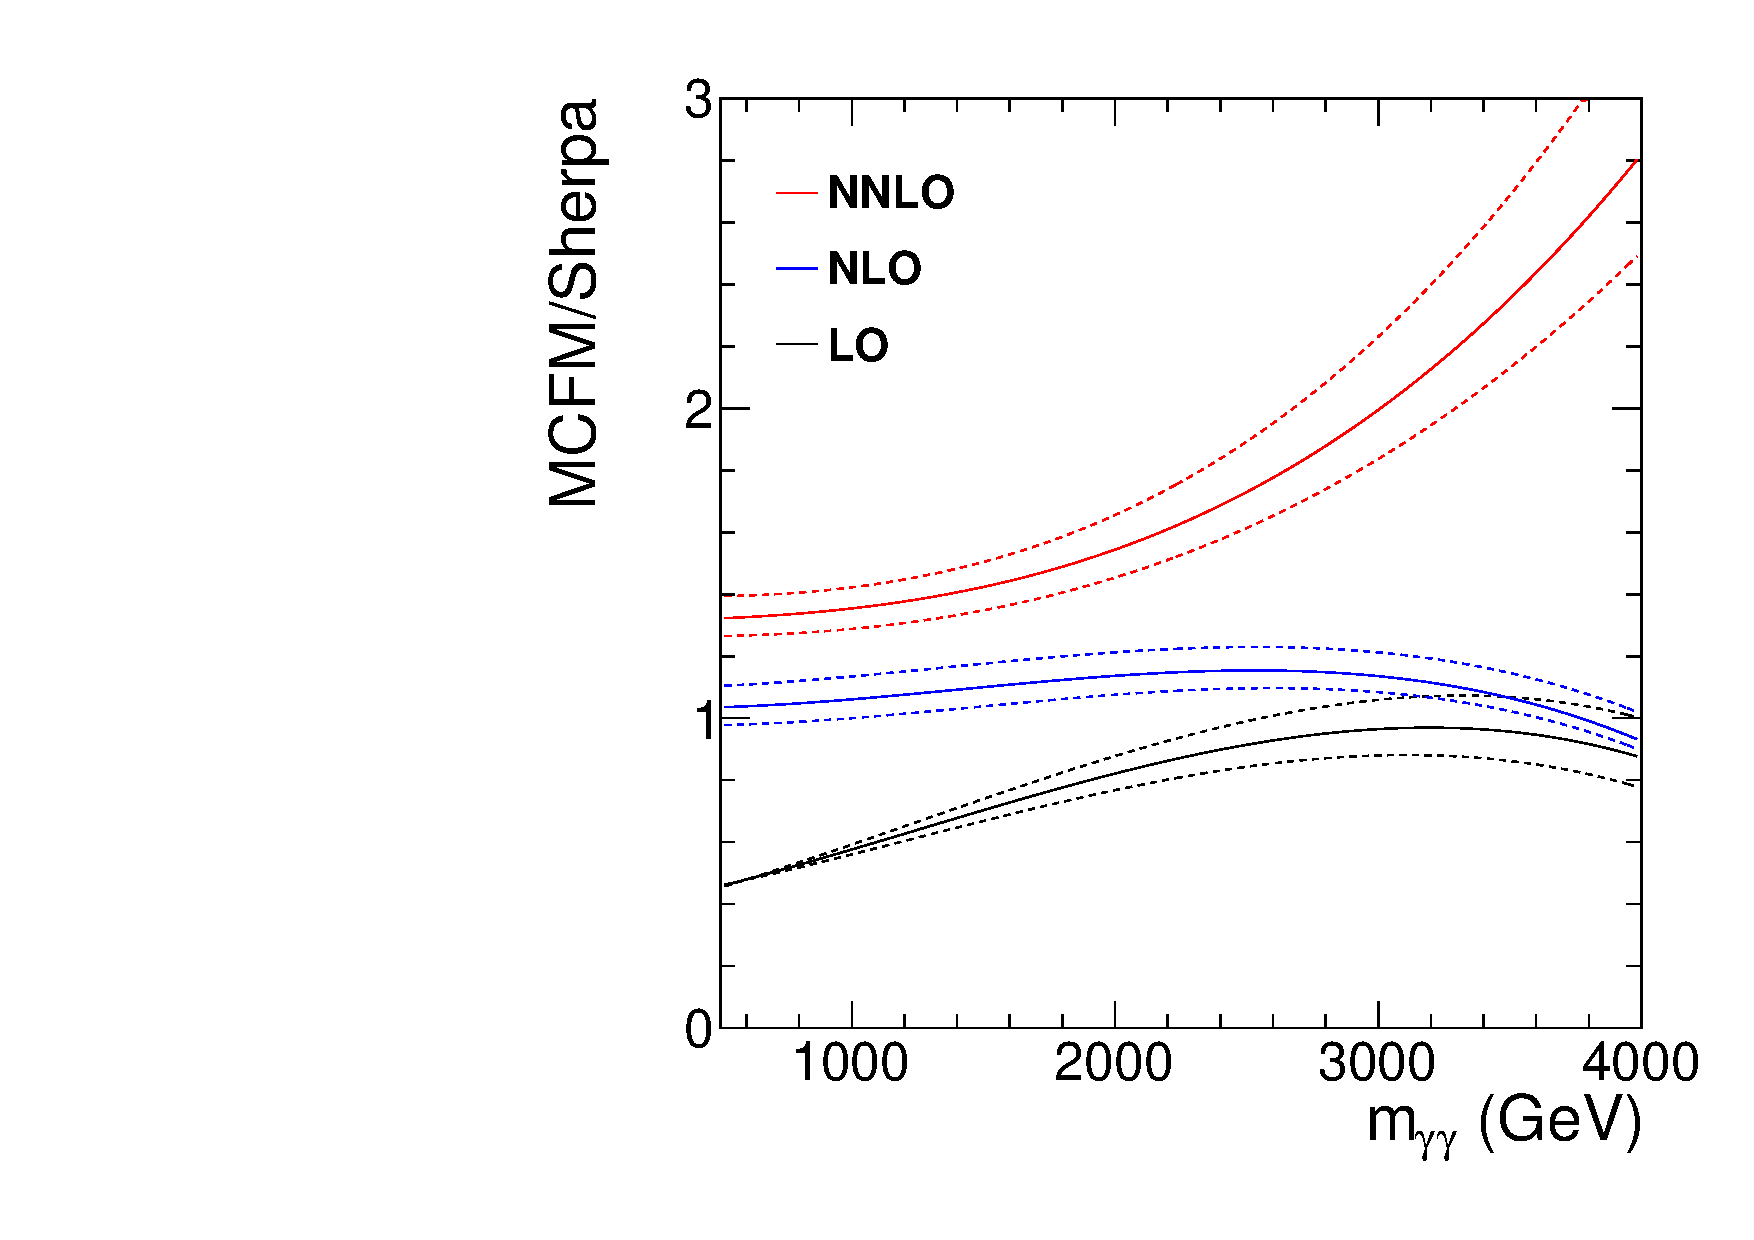
\includegraphics[angle=0,width=0.45\textwidth]{fig/kfactor_comparison_BB_125GeV_NNPDF.pdf}
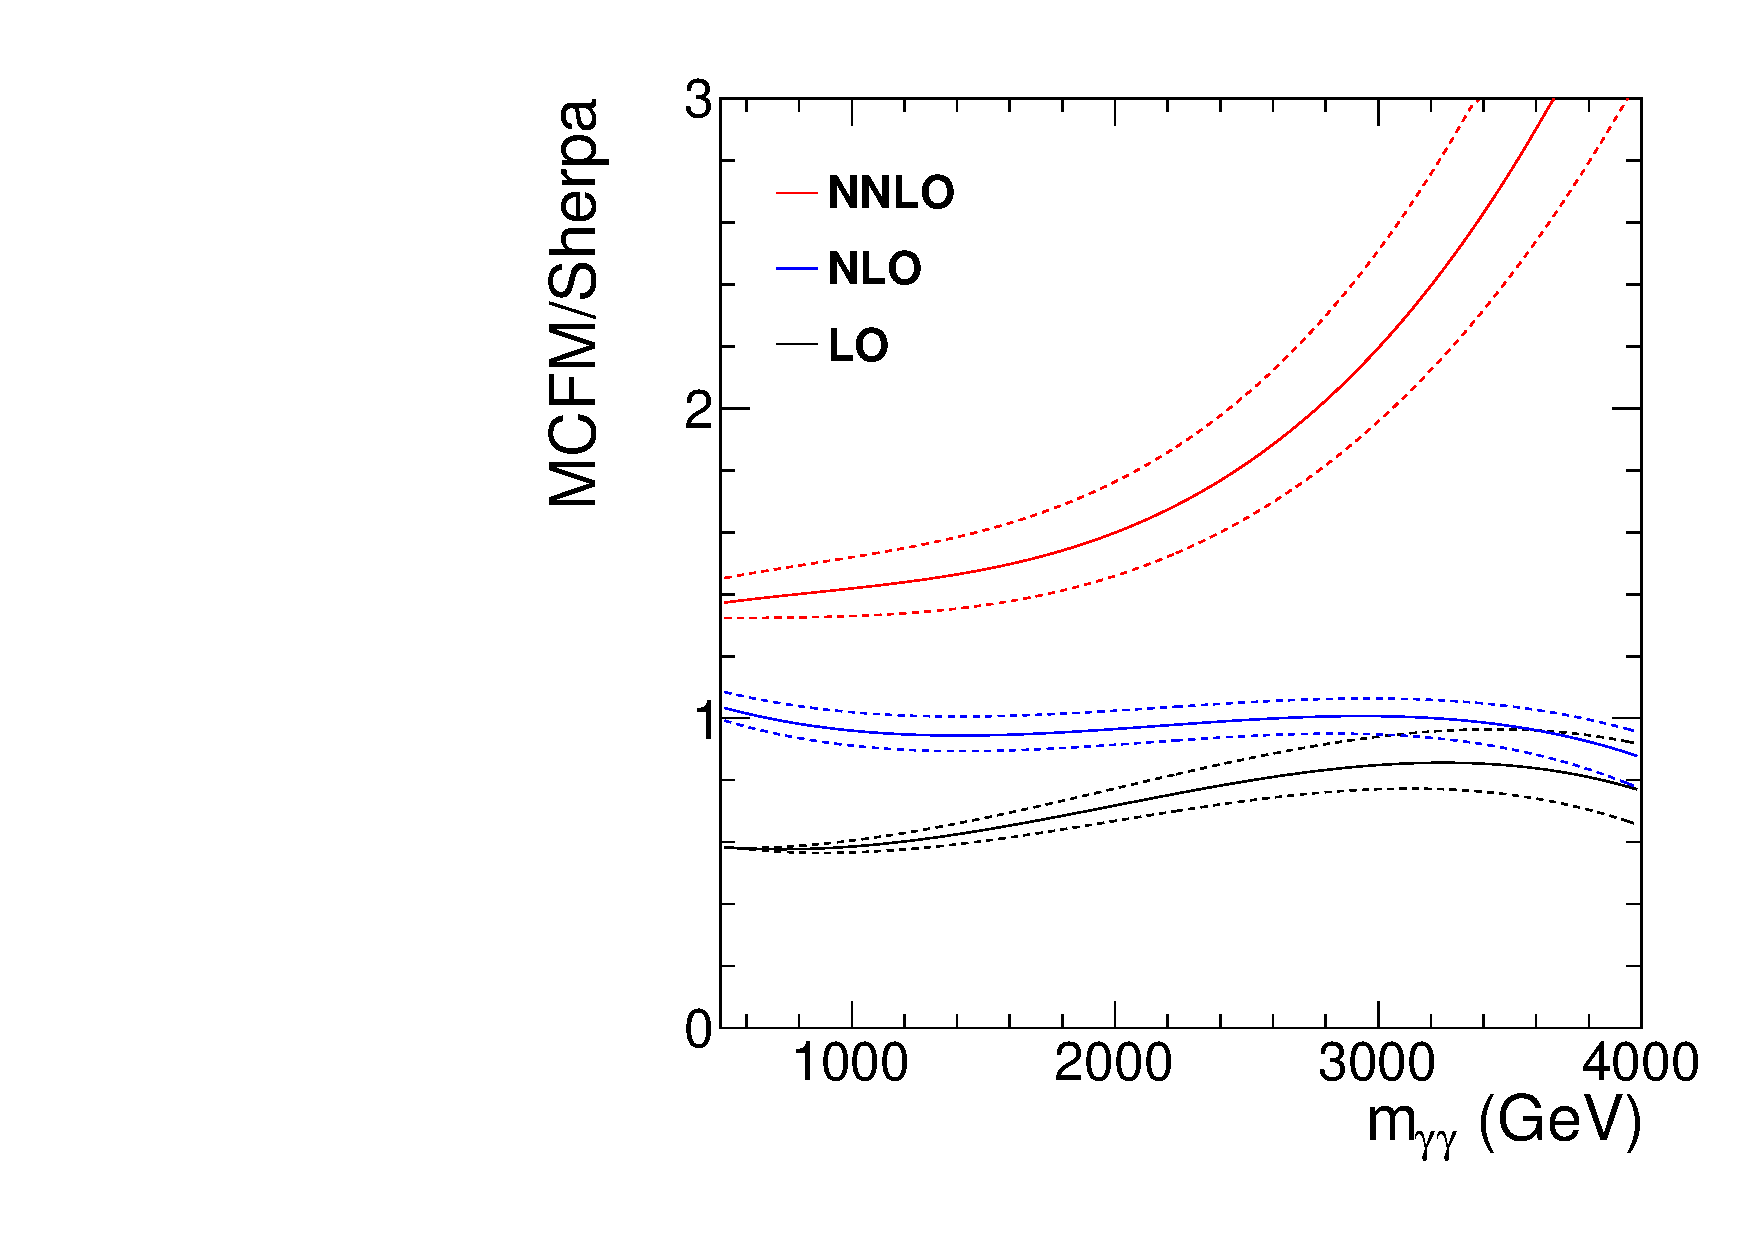
\includegraphics[angle=0,width=0.45\textwidth]{fig/kfactor_comparison_BE_125GeV_NNPDF.pdf}
\end{center}
\label{fig:kfactor_comparison}
\end{figure}

Figure~\ref{fig:kfactor_comparison} shows a summary of the ratios of the diphoton cross section from MCFM to that from \SHERPA. Different orders of the MCFM calculation are shown and the dashed lines show the variation of the renormalization and factorization scales as shown in Figure~\ref{fig:kfactor_mgg}. The nominal ratios are shown in full lines while the dashed lines show the effect of the simultaneous renormalization and factorization variations. This effect is treated as a systematic uncertainty and will be discussed more in Ch.~\ref{ch:systematics}. 

In MCFM, the fragmentation scale is set to the renormalization scale by default. The fragmentation scale is the scale of the fragmentation functions that describe the probability for a parton to fragment into a hadron. This contribution is negligible when using the Frixione isolation which is discussed more in \cite{Frixione:1998jh}. The fragmentation scale is a parameter that describes the energy scale at which a high-energy quark or gluon (parton) fragments into a jet of hadrons, which are composite particles made up of quarks and gluons. Note that the fragmentation scale and the renormalization scale are both important concepts in theoretical particle physics, but they refer to different aspects of the theory. The fragmentation process is a non-perturbative phenomenon, which means it cannot be calculated using standard perturbative techniques. Instead, it is described using phenomenological models that are tuned to experimental data. The fragmentation scale is typically on the order of a few GeV to tens of GeV, depending on the process being studied. The renormalization scale, on the other hand, is a parameter that describes the energy scale at which the coupling constants in the theory are defined. In quantum field theory, the coupling constants are typically dependent on the energy scale at which they are probed. This is due to the effects of virtual particles that are created and annihilated in the vacuum. To account for these effects, the coupling constants are "renormalized", which means they are adjusted at different energy scales to remove divergences in the theory. The renormalization scale is typically chosen to be on the order of the energy scale at which the process of interest is taking place. In summary, the fragmentation scale and the renormalization scale are two different energy scales that are used in different contexts in theoretical particle physics. The fragmentation scale is used to describe the energy scale at which partons fragment into hadrons, while the renormalization scale is used to describe the energy scale at which the coupling constants in the theory are defined.

The \texttt{NNPDF30\_NNLO\_as\_0118} set of parton distribution functions (PDFs) are used~\cite{Ball:2014uwa}. \SHERPA includes the contribution of prompt photons from gluon and quark partons fragmenting to photons, which avoids the necessity of imposing an arbitrary $\Delta R$ selection between photons and jets to avoid infrared divergences~\cite{Hoeche:2009xc}. Infrared divergence is a phenomenon that arises in quantum field theory when the energies of the particles involved in a scattering process become very low. In particular, infrared divergence occurs when the energy of a particle becomes much smaller than the mass of the particle. 
The photons are required to satisfy $p_{T} > 50 \GeV$ at generator level.

As described later in Section~\ref{sec:bkg_real}, these simulated diphoton+jets events will be reweighted by the NNLO k-factor to provide our prediction to the irreducible diphoton background. 
The photon+jet samples listed in Table~\ref{table:mcbackgroundsamples} are used only for studies such as the MC closure test, cross-checking of fake predictions and deriving templates for real photons (helped by large statistics), but are not part of the final background prediction, which is data-driven for fakes. We list them here only for completeness. Also listed in Table~\ref{table:mcbackgroundsamples} are a separate set of leading-order-only MC background samples which were also generated with \PYTHIA~8.2~\cite{Sjostrand:2008za} with the \texttt{NNPDF}3.1 LO set of parton distribution functions as found in the event tune, \texttt{TuneCP2}~\cite{Sirunyan:2019dfx}. This LO diphoton set is used only for subtracting the background from the signal samples that are generated with the same generator and PDF. This takes into account the effect of interference between signal and background. 

While minor backgrounds arise from other SM processes, we have not included them in this analysis as their effects are negligible. The processing configuration (Campaign and Global Tag, by year) for all MC samples in this analysis is listed in Table~\ref{table:mcdatasets2016-18}.


% In addition to the SM diphoton process, minor backgrounds arise from other SM processes which can produce the diphoton signature if one or more object leaves a fake photon signature. Such processes include $(\PW/\PZ)\PGg$+jets, Drell-Yan, and $\PQt\PAQt\PGg$. Since these background contributions are found to be small in the diphoton final state, we estimate them directly from MC. The MC samples used for these minor backgrounds are listed in Table~\ref{table:minorbackgroundsamples}. These processes were mostly generated with MADGRAPH, although some used \PYTHIA.
% The tune used for these minor background samples was \texttt{TuneCUETP8M1} for 2016 data and \texttt{TuneCP2} for 2017--2018 data.





% \begin{landscape}
% \begin{table}[!htbp]
%       \caption{Minor background samples used in the analysis. Here XXX stands for RunIISummer16MiniAODv3-PUMoriond17\_94X\_mcRun2\_asymptotic\_v3 for 2016 samples, RunIIFall17MiniAODv2-PU2017\_12Apr2018\_94X\_mc2017\_realistic\_v14 for 2017 samples or RunIIAutumn18MiniAOD-102X\_upgrade2018\_realistic\_v15-v1 for 2018 samples. The subdivisions of the table correspond to, from top to bottom, the 2016, 2017 and 2018 datasets used in the analysis.
%       %YYY for RunIIFall17MiniAOD-94X\_mc2017\_realistic\_v10All
%   % ZZZ for RunIIFall17MiniAODv2-PU2017\_12Apr2018\_94X\_mc2017\_realistic\_v14/.
%       }
%       \centering
%       \vspace{\baselineskip}
%       \begin{tabular}{lc}
%       \hline \hline
%       Data set path & Cross section (pb)\\
%       \hline
% /WGJets\_MonoPhoton\_PtG-40to130\_TuneCUETP8M1\_13TeV-madgraph/XXX & 1.270e+01\\
% /WGJets\_MonoPhoton\_PtG-130\_TuneCUETP8M1\_13TeV-madgraph/XXX & 6.565e-01\\
% /ZGTo2LG\_TuneCUETP8M1\_13TeV-amcatnloFXFX-pythia8/XXX & 117.864\\
% /DYJetsToLL\_M-50\_HT-*\_TuneCUETP8M1\_13TeV-madgraphMLM-pythia8/XXX & Varies \\
% /TTGamma\_Hadronic\_ptGamma100-200\_TuneCP5\_PSweights\_13TeV-madgraph-pythia8/XXX & 1.251e-01\\
% /TTGamma\_Hadronic\_ptGamma200inf\_TuneCP5\_PSweights\_13TeV-madgraph-pythia8/XXX & 2.687e-02\\
% /TTGamma\_SingleLept\_ptGamma100-200\_TuneCP5\_PSweights\_13TeV-madgraph-pythia8/XXX & 1.320e-01\\
% /TTGamma\_SingleLept\_ptGamma200inf\_TuneCP5\_PSweights\_13TeV-madgraph-pythia8/XXX & 2.703e-02\\
% /TTGamma\_Dilept\_ptGamma100-200\_TuneCP5\_PSweights\_13TeV-madgraph-pythia8/XXX & 3.428e-02\\
% /TTGamma\_Dilept\_ptGamma200inf\_TuneCP5\_PSweights\_13TeV-madgraph-pythia8/XXX & 6.797e-03 \\
% \hline
% /WGJets\_MonoPhoton\_PtG-40to130\_TuneCP5\_13TeV-madgraph/XXX & 7.163e-01\\
% /WGJets\_MonoPhoton\_PtG-130\_TuneCP5\_13TeV-madgraph/XXX & 7.152e-01\\
% /ZGToLLG\_01J\_5f\_TuneCP5\_13TeV-amcatnloFXFX-pythia8/XXX & 5.559e+01\\
% /DYJetsToLL\_M-50\_HT-*\_TuneCP5\_13TeV-madgraphMLM-pythia8/XXX & Varies\\
% /TTGamma\_Hadronic\_ptGamma100-200\_TuneCP5\_PSweights\_13TeV-madgraph-pythia8/XXX & 1.251e-01\\
% /TTGamma\_Hadronic\_ptGamma200inf\_TuneCP5\_PSweights\_13TeV-madgraph-pythia8/XXX & 2.687e-02\\
% /TTGamma\_SingleLept\_ptGamma100-200\_TuneCP5\_PSweights\_13TeV-madgraph-pythia8/XXX & 1.320e-01\\
% /TTGamma\_SingleLept\_ptGamma200inf\_TuneCP5\_PSweights\_13TeV-madgraph-pythia8/XXX & 2.703e-02\\
% /TTGamma\_Dilept\_ptGamma100-200\_TuneCP5\_PSweights\_13TeV-madgraph-pythia8/XXX & 3.428e-02\\
% /TTGamma\_Dilept\_ptGamma200inf\_TuneCP5\_PSweights\_13TeV-madgraph-pythia8/XXX & 6.797e-03\\
% \hline
% /WGJets\_MonoPhoton\_PtG-40to130\_TuneCP5\_13TeV-madgraph/XXX & 7.163e-01\\
% /WGJets\_MonoPhoton\_PtG-130\_TuneCP5\_13TeV-madgraph/XXX & 7.152e-01\\
% /ZGToLLG\_01J\_5f\_TuneCP5\_13TeV-amcatnloFXFX-pythia8/XXX & 5.559e+01\\
% /DYJetsToLL\_M-50\_HT-*\_TuneCP5\_PSweights\_13TeV-madgraphMLM-pythia8/XXX & Varies\\
% /TTGamma\_Hadronic\_ptGamma100-200\_TuneCP5\_13TeV-madgraph-pythia8/XXX & 1.256e-01\\
% /TTGamma\_Hadronic\_ptGamma200inf\_TuneCP5\_13TeV-madgraph-pythia8/XXX & 2.678e-02\\
% /TTGamma\_SingleLept\_ptGamma100-200\_TuneCP5\_13TeV-madgraph-pythia8/XXX & 1.320e-01\\
% /TTGamma\_SingleLept\_ptGamma200inf\_TuneCP5\_13TeV-madgraph-pythia8/XXX & 2.703e-02\\
% /TTGamma\_Dilept\_ptGamma100-200\_TuneCP5\_13TeV-madgraph-pythia8/XXX & 3.427e-02\\
% /TTGamma\_Dilept\_ptGamma200inf\_TuneCP5\_13TeV-madgraph-pythia8/XXX & 6.800e-03\\
%       \hline \hline
%       \end{tabular}
%       \label{table:minorbackgroundsamples}
% \end{table}
% \end{landscape}





\section{Background from Fake Photons}\label{sec:bkg_fake}


\begin{figure}[htbp!]
\caption{Schematic of a $\pi^{0}$ decaying into two photons that deposit energy that mimics energy-deposit features of prompt photons.}
\begin{center}
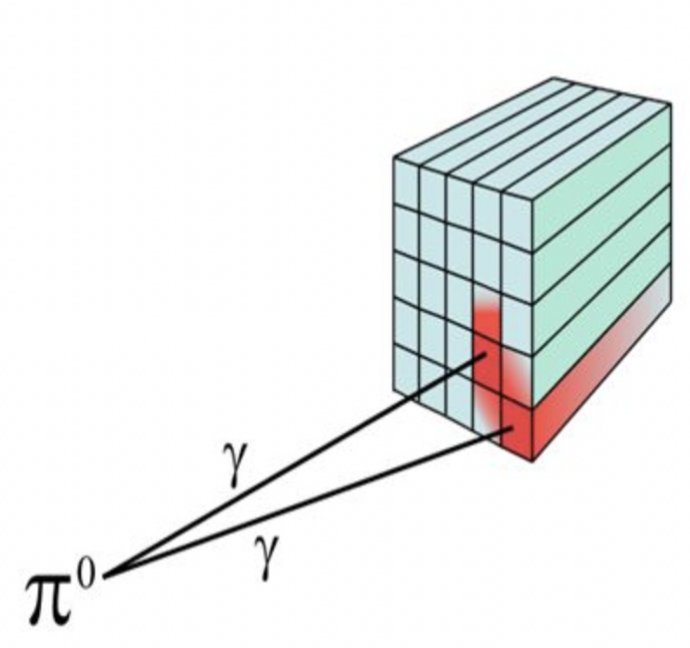
\includegraphics[angle=0,width=0.7\textwidth]{fig/SchematicOfJetFakingPhoton.png}
\end{center}
\label{fig:pi0Decay}
\end{figure}
% \subsection{Overview of Photon Fake Rate Method}

Another source of background in the diphoton signal region comes from 'fake photons'. This term is assigned to events where one or two jets are misidentified as 'real' photons by virtue of passing the high $p_T$ ID. This occurs when jets fragments in such a way that when they decay to two photons; and at sufficiently high momentum they overlap in the detector and resemble a single photon signature. Such jet fragmentation typically happens with $\pi^{0}$ or another neutral meson decaying into two photons~\ref{fig:pi0Decay}. A neutral meson that has little hadronic activity around it can also be reconsturcted that can pass the photon isolation criteria and be mislabeled as a photon. 


% If at the same time there is little hadronic activity around the neutral meson, the reconstructed object can pass the isolation and other identification criteria and could be mislabeled as a 'photon' in our analysis. To estimate this 'fake' contribution, we use a data-based method rather than just MC simulation for such a rare jet fragmentation  process. This method is similar to that used to a previously published analysis of 2016 diphoton data~\cite{Sirunyan:2018wnk} and in the 8 TeV exotica diphoton analysis~\cite{CMS-PAS-EXO-12-045}.

The method used to estimate the 'fake' contribution assumes that dijet or $\gamma + j$ events where these jets fragmented in such a way to produce a fake photon signature could be modeled by other such events where the jet fragmented differently. Here we define two distinct categories of jet fragmentation which we measure. The ratio of these two categories provide us the 'fake rate'. 

The first category, the numerator, are jets that pass the high-\pt photon ID requirements specified in Table~\ref{table:highptid}. The denominator category, consist of 'photon-like' jets which pass an less strict version of the photon ID requirements, and are additionally required to fail at least one of the other photon ID requirements. The latter requirement ensures, that the numerator and denominator are orthogonal, i.e. there is no contamination from real photons in the denominator. The complete set of denominator selection criteria is given in Table~\ref{tab:fake_rate_cuts}. 

\begin{table}[!htbp]
\caption{Fake rate definitions, where fake rate = numerator / denominator. The real and fake templates are fit to the numerator candidates using the template variable labeled `template'.
 After the fitting procedure is performed, the cut associated with the template variable is applied. The photon ID is shown for comparison.}
\label{tab:fake_rate_cuts}

  % \caption{The cut-based definitions of the numerator and denominator objects for the fake rate calculation compared against the high-\pt photon ID. The numerator is determined after numerator candidates are fit with real and fake templates (definitions shown) using the template variable \sieie. The cuts listed are for both the EB and EE regions unless separately specified.}
  % \label{tab:fake_rate_cuts}
  \centering
  \vspace{\baselineskip}
  \tiny
  \begin{tabular}{l|cccccc}
  \hline \hline
  Cut [EB \{sat.\} (EE \{sat.\})] & Photon ID & Num. & Real template & Fake template & Denom. (EB) & Denom. (EE) \\
  \hline
   & & & & & & \\
  \textbf{Photon ID cuts} & & & & & & \\
  \hline
  $\hoe < 0.05$ & pass & pass & pass & pass & \multirow{5}{*}{fail at least one} &  \multirow{4}{*}{fail at least one} \\
  $\sieie < 0.0105\, \{0.0112\}\, (0.028\, \{0.030\})$ & pass & template & template & template & & \\
  $\chiso < 5\GeV$ & pass & pass & pass & not applied & & \\
  $\corphoiso < 2.75\, (2.00)\GeV$ & pass & pass & pass & pass & & pass \\
  $\rnine > 0.8$ & pass & pass & pass & pass & pass & pass \\
   & & & & & & \\
  \textbf{Electron veto} & & & & & & \\
  \hline
  CSEV & pass & pass & pass & pass & pass & pass \\
   & & & & & & \\
  \textbf{Additional fake rate cuts} & & & & & & \\
  \hline
  $\sigma_{i\phi i\phi} > 0.009$ & not applied & pass & pass & pass & pass & pass \\
  $5 < \chiso < 10\GeV$ & not applied & not applied & not applied & pass & not applied & not applied \\
  $\text{Hadronic/E} < 0.1$ & not applied & not applied & not applied & not applied & pass & pass \\
  $\chiso < 0.2\,\pt$ & not applied & not applied & not applied & not applied & pass & pass \\
  $\corphoiso < 0.2\,\pt$ & not applied & not applied & not applied & not applied & pass & not applied \\
  \hline \hline
  \end{tabular}
\end{table}

% \begin{table}[p]

% \begin{center}
% \tiny
% \begin{tabular}{l|cccccc}
% \hline \hline
% Cut [EB \{sat.\} (EE \{sat.\})] & High \pt photon ID & Numerator candidates & Real template & Fake template & Denominator (EB) & Denominator (EE) \\
% \hline
%  & & & & & & \\
% \textbf{High $\pt$ photon ID cuts} & & & & & & \\
% \hline
% $H/E < 0.05$ & pass & pass & pass & pass & \multirow{5}{*}{fail at least one} &  \multirow{4}{*}{fail at least one} \\
% $\sieie < 0.0105 \{0.0112\} (0.028 \{0.030\})$ & pass & template & template & template & & \\
% $\chiso < 5 \GeV$ & pass & pass & pass & not applied & & \\
% $\overline{Iso_{\gamma}} < 2.75 (2.00) \GeV$ & pass & pass & pass & pass & & pass \\
% $\RNINE > 0.8$ & pass & pass & pass & pass & pass & pass \\
%  & & & & & & \\
% \textbf{Electron veto} & & & & & & \\
% \hline
% CSEV & pass & pass & pass & pass & pass & pass \\
%  & & & & & & \\
% \textbf{Additional cuts for fake rate} & & & & & & \\
% \hline
% $\sigma_{i\phi i\phi} > 0.009$ & not applied & pass & pass & pass & pass & pass \\
% $5 < \chiso < 10 \GeV$ & not applied & not applied & not applied & pass & not applied & not applied \\
% $Hadronic/E < 0.1$ & not applied & not applied & not applied & not applied & pass & pass \\
% $\chiso < 0.2 \pt$ & not applied & not applied & not applied & not applied & pass & pass \\
% $\overline{Iso_{\gamma}} < 0.2 \pt$ & not applied & not applied & not applied & not applied & pass & not applied \\
% \hline \hline
% \end{tabular}
% \end{center}
% \end{table}

What we seek to measure, termed the \emph{fake rate}, is defined as 

\begin{equation} \label{eq:fakeRate}
f=\frac{\mbox{number of jets passing high \pt ID}}{\mbox{number of jets passing denominator definition}}
\end{equation}

Note that this ``fake rate" is just a relative ratio between two distinct categories of jet fragmentation, not the rate at which a generic jet fakes a photon, which is actually much smaller. The ``fake rate" is measured in a reference data sample as a function of the photon \pt, $\eta$ and the number of primary vertices. Events containing a denominator jet are taken to be representative of other possible events where the jets could have fragmented in a way that they pass the photon ID. To obtain the ``fake contribution", we take the data events containing objects that pass the pass the looser ``photon-like jet" denominator definition and reweight them by the fake rate. 

\subsection{Subtracting Real Photon Contamination in the Fake Rate}

In measuring the fake rate in Eq.~\ref{eq:fakeRate}, a complication arises in the determination of the numerator. The set of objects selected from data which pass the photon ID criteria will include both jets and real photons. This real photon contribution must be subtracted since our definition of the fake rate are from jets-faking-photons counts. The general procedure for subtracting this real photon contamination in the numerator is as follows. We consider a photon ID variable (such as shower-shape, \sieie which is sensitive to the difference between real and fake photons. We relax the cut on this variable, specified in Table~\ref{tab:fake_rate_cuts} as \texttt{template} and plot the distribution of this variable for all objects which otherwise pass the rest of the numerator ID. Shower-shape templates are constructed for both real and fake photons and then these templates are fit to the observed data. The fit allows us to determine the fraction of photons which are real/fake after applying the ID cut on the fitting variable. We then calculate the number we should use for our numerator in the fake rate. Because the variable distributions typically vary with $p_{T}$, this fitting and subtractions is done per \pt bin. 

The following sections describe this procedure in more detail. Closure tests that validate this procedure are described further in Section~\ref{sec:closure_test}. In the closure test, we found that splitting the barrel and endcap regions into inner and outer regions further improved the fake prediction. This is an improvement over the previous analysis in Ref.~\cite{cmsdiphoton2016}.

\subsection{Fake Rate Numerator: Templates and Fitting}

The fake rate in our analysis is defined as a ratio of strictly jets-which-fragmented-to-pass-photon-ID to jets-which-fragmented-to-pass-a-looser-ID. When we run through the data to measure the numerator, i.e. jets-which-fragmented-to-pass-photon-ID, we inevitably select real photons. To subtract this real photon contamination, we use a template fit to a variable that is sensitive to the difference between real and fake photons. Here we use the \sieie variable to form real and fake template distributions. 

%%real template
We construct the real photon \sieie distributions from MC \texttt{GGjets} samples that are listed in Section~\ref{sec:datasets}). The reconstructed photon object is required to match in $\Delta R$ to a GenParticle photon before being used to form the template.

%%Fake template ...
We derive the fake template from the \texttt{JetHT} dataset which provides a large supply of 'fake photons' from jets. These constructed fake templates are then used to fit separately to the \texttt{JetHT} or \texttt{DoubleMuon} datasets. Table~\ref{table:dset-JetHTFakeRate} and ~\ref{table:dset-DoubleMuonFakeRate} show the \JetHT and \DoubleMuon data sets, respectively.

We select a sideband sample of objects that pass most of the Photon ID, but are required to have a charged hadron isolation value in the sideband of $5<\chiso<10$\GeV. The idea behind the sideband is to select objects which still has similar properties to the ``fake" objects that pass the Photon ID. By requiring the objects to fail \chiso cut, makes the sample fake-enriched. The \chiso variable is chosen to define the sideband sample because it is the ID variable which is \emph{least} correlated with the \sieie template variable. There is still some unavoidable correlation between these variables. This is because of the physics of jet fragmentation which tends to produce high-EM content (via decays of neutral mesons) also tends to produce charged hadrons which contribute to the isolation variable. Using a different sideband definition will unavoidable sculpt the extracted \sieie template to some degree. To minimize the bias, we choose a sideband which is as close as possible to the cut value for passing the real photon ID. We then explore the variation in template shape that is obtained by using different sideband definitions. This is a source of systematic uncertainty on the fake rate method which will be discussed later in Ch.~\ref{ch:systematics}. 

% %%pt dependence ...
% The real and fake templates vary with \pt therefore, we generate templates in different \pt bins. 
Figure~\ref{fig:real_templates} and Figure~\ref{fig:fake_templates} show the \pt dependence or variation among the real and fake templates, respectively in both the EB and EE. The template fit to the \texttt{JetHT} or \texttt{DoubleMuon} datasets are then performed separately in each \pt bin.

% % generated by FakeRateAnalysis/RooFitTemplateFitting/analysis/makePlotsNew.py
\begin{figure}[!htbp]
\caption{Representative real templates derived from MC in EB and EE for different \pt bins.}
\centering
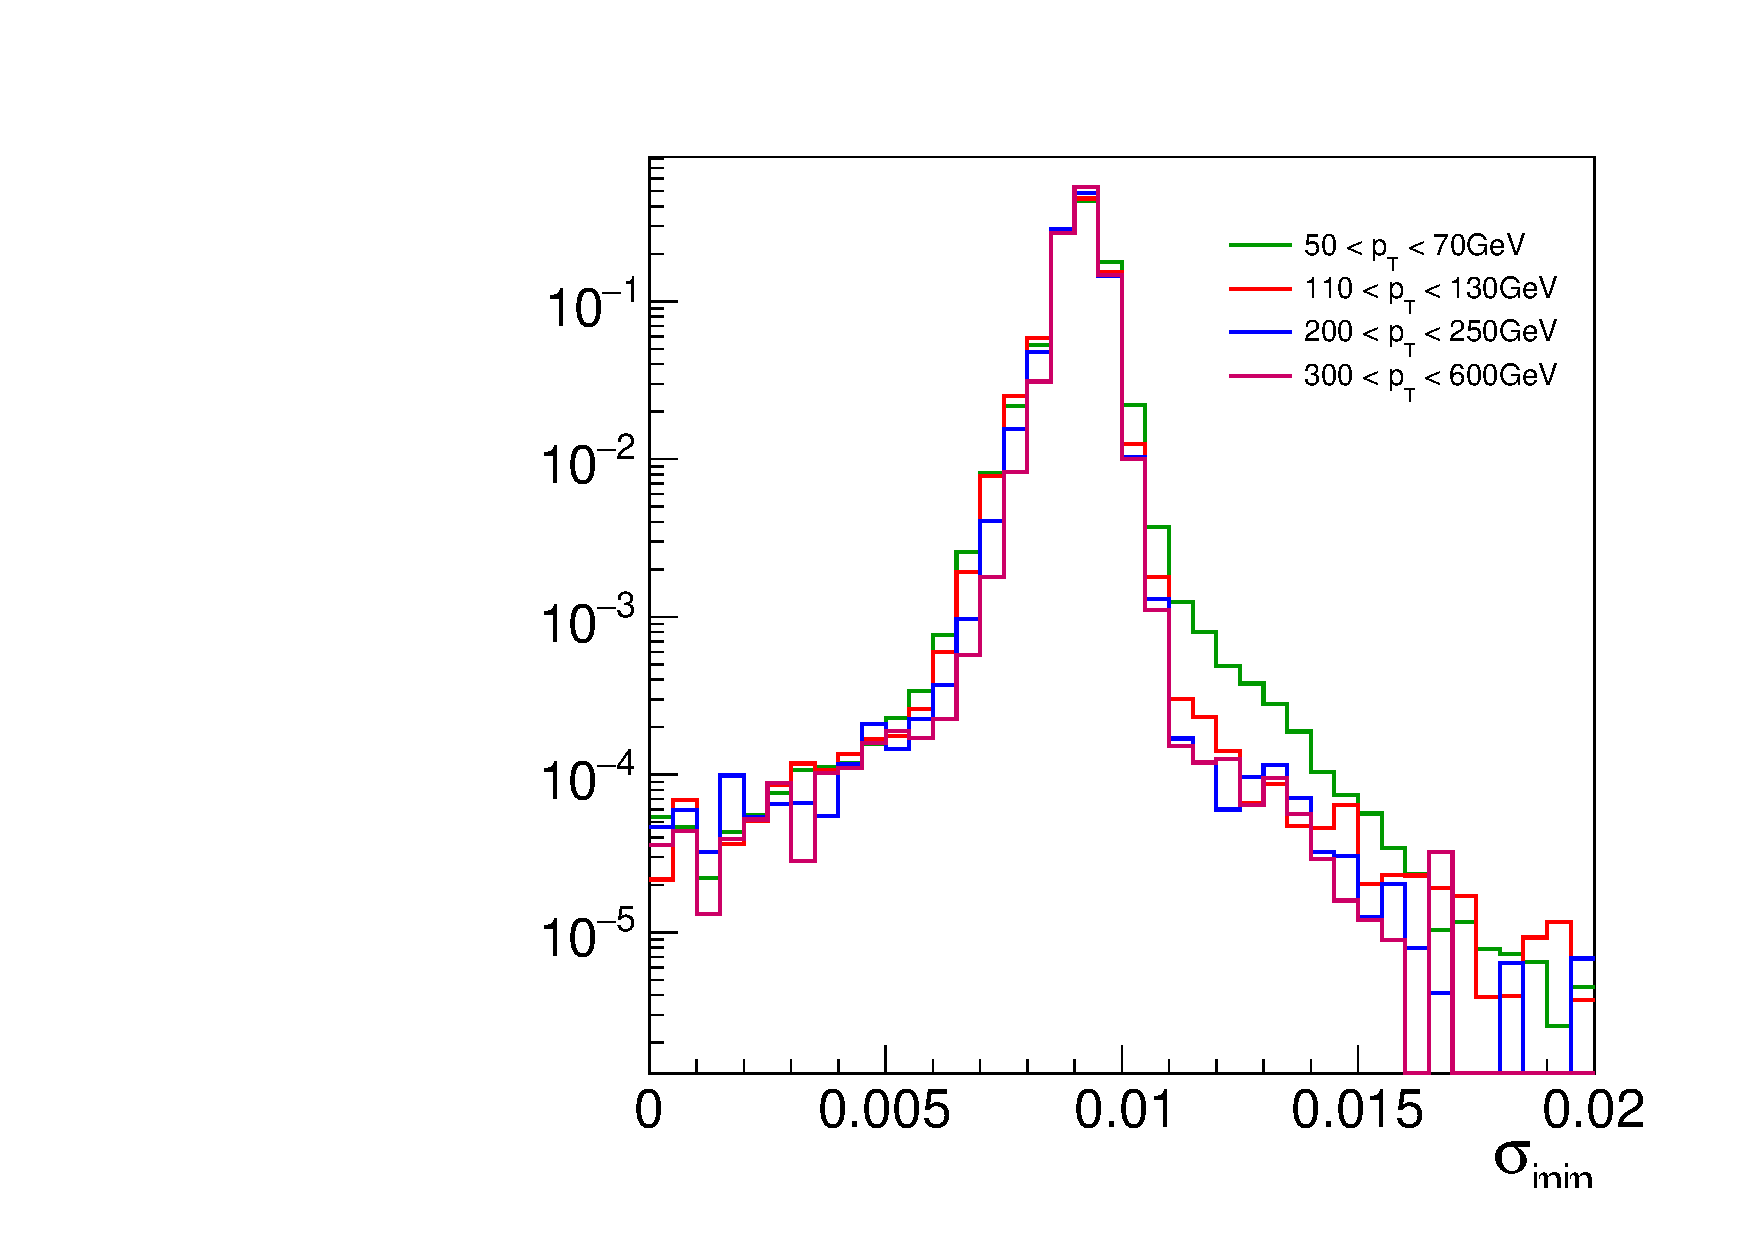
\includegraphics[width=0.49\textwidth]{fig/realtemplatecompEB_2018.pdf}
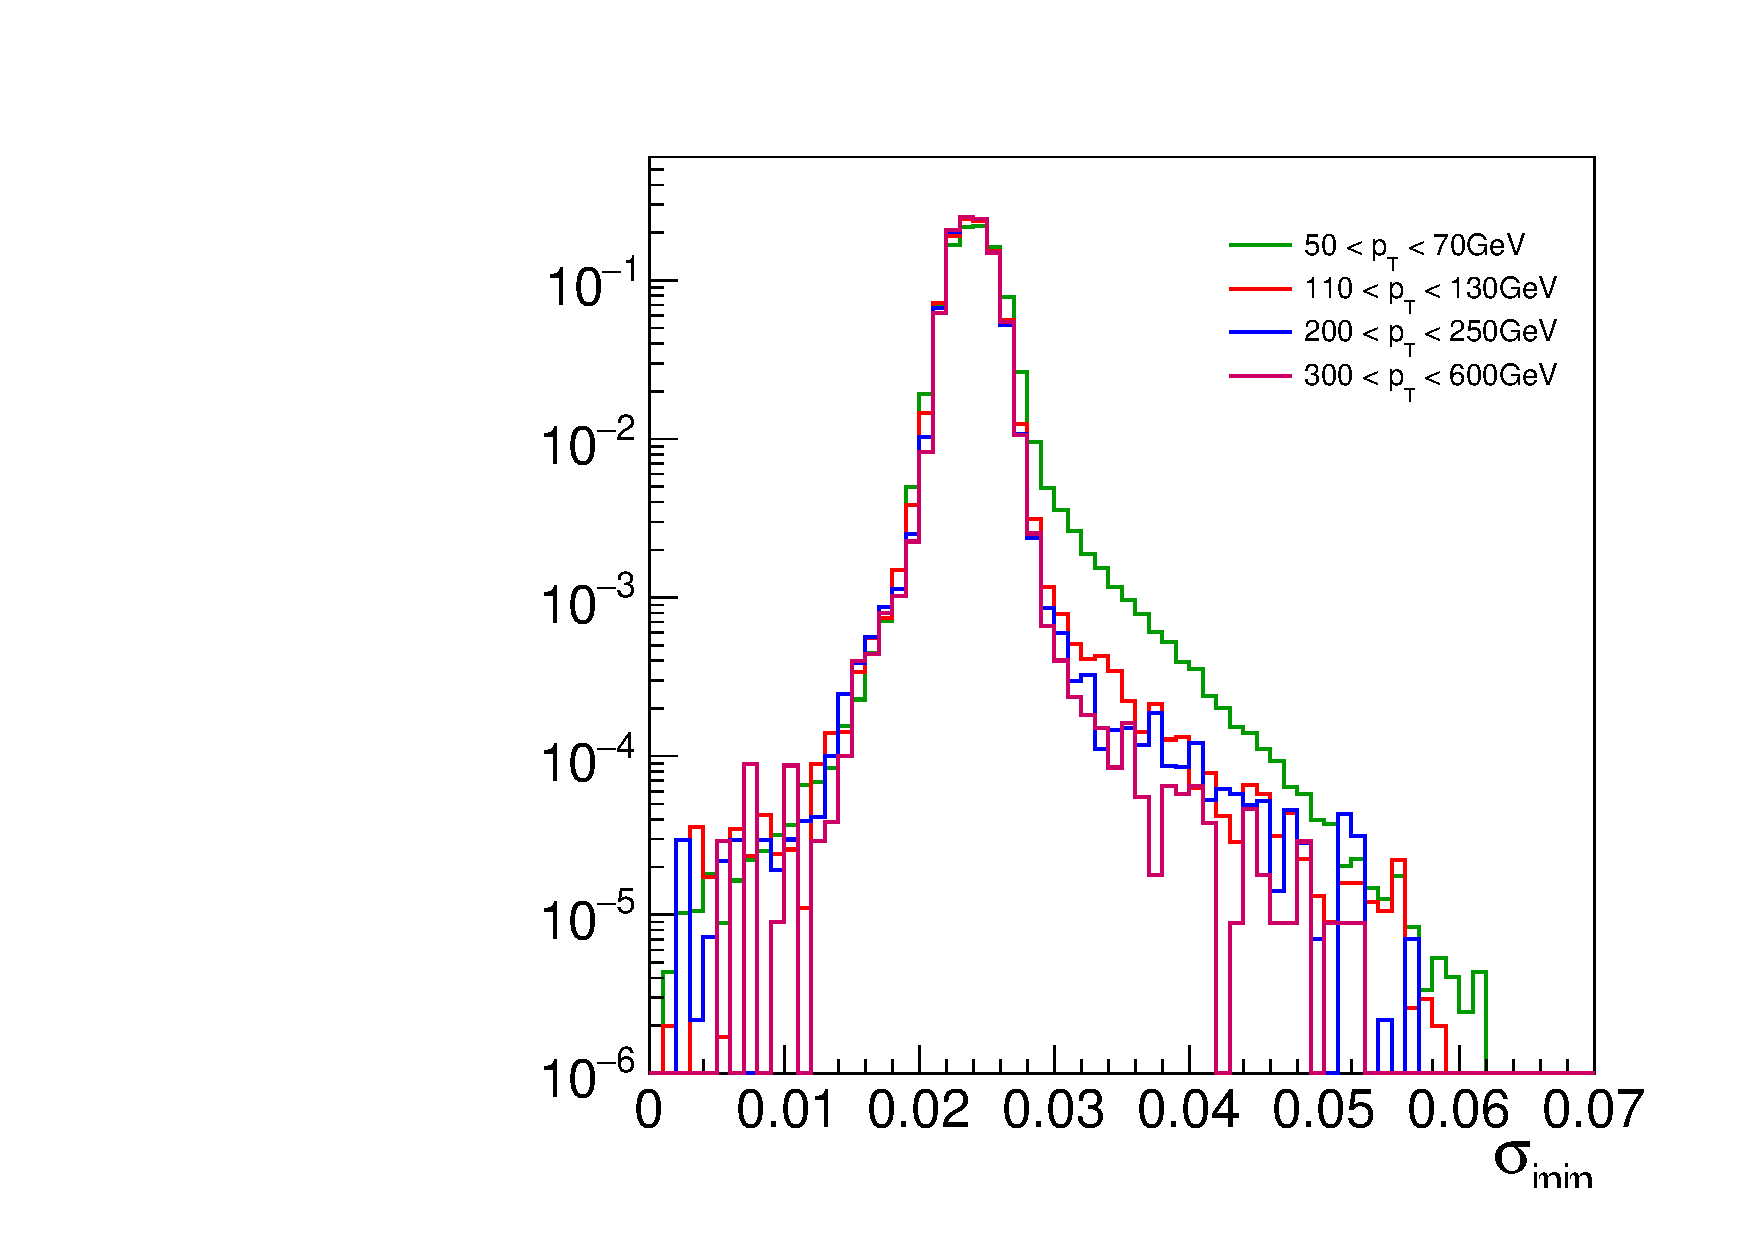
\includegraphics[width=0.49\textwidth]{fig/realtemplatecompEE_2018.pdf}
\label{fig:real_templates}
\end{figure}

% % % generated by FakeRateAnalysis/RooFitTemplateFitting/analysis/makePlotsNew.py
\begin{figure}[!htbp]
\caption{Fake templates comparison measured in various \pt bins extracted from the \texttt{JetHT} data set for EB (left) and EE (right).}
\centering
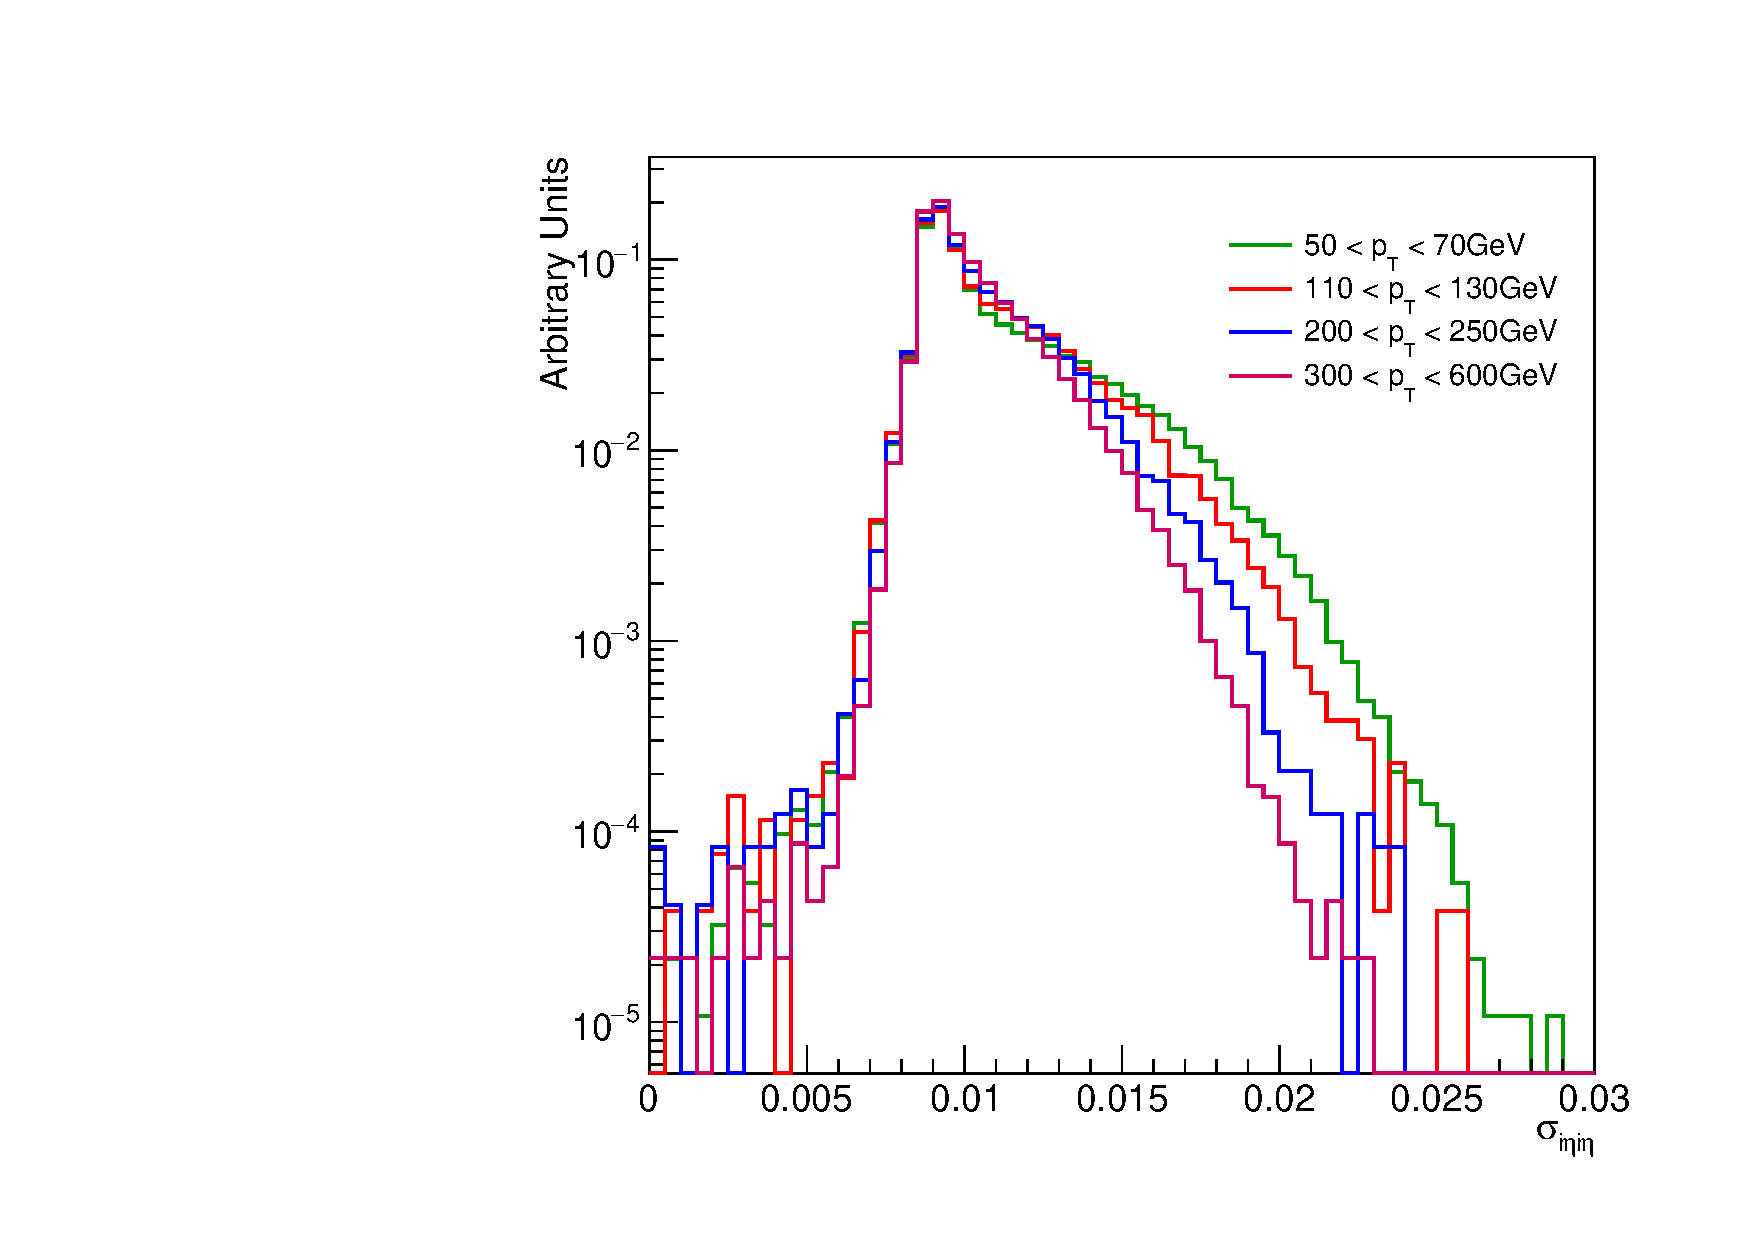
\includegraphics[width=0.49\textwidth]{fig/faketemplatecompEB_jetht_2018.pdf}
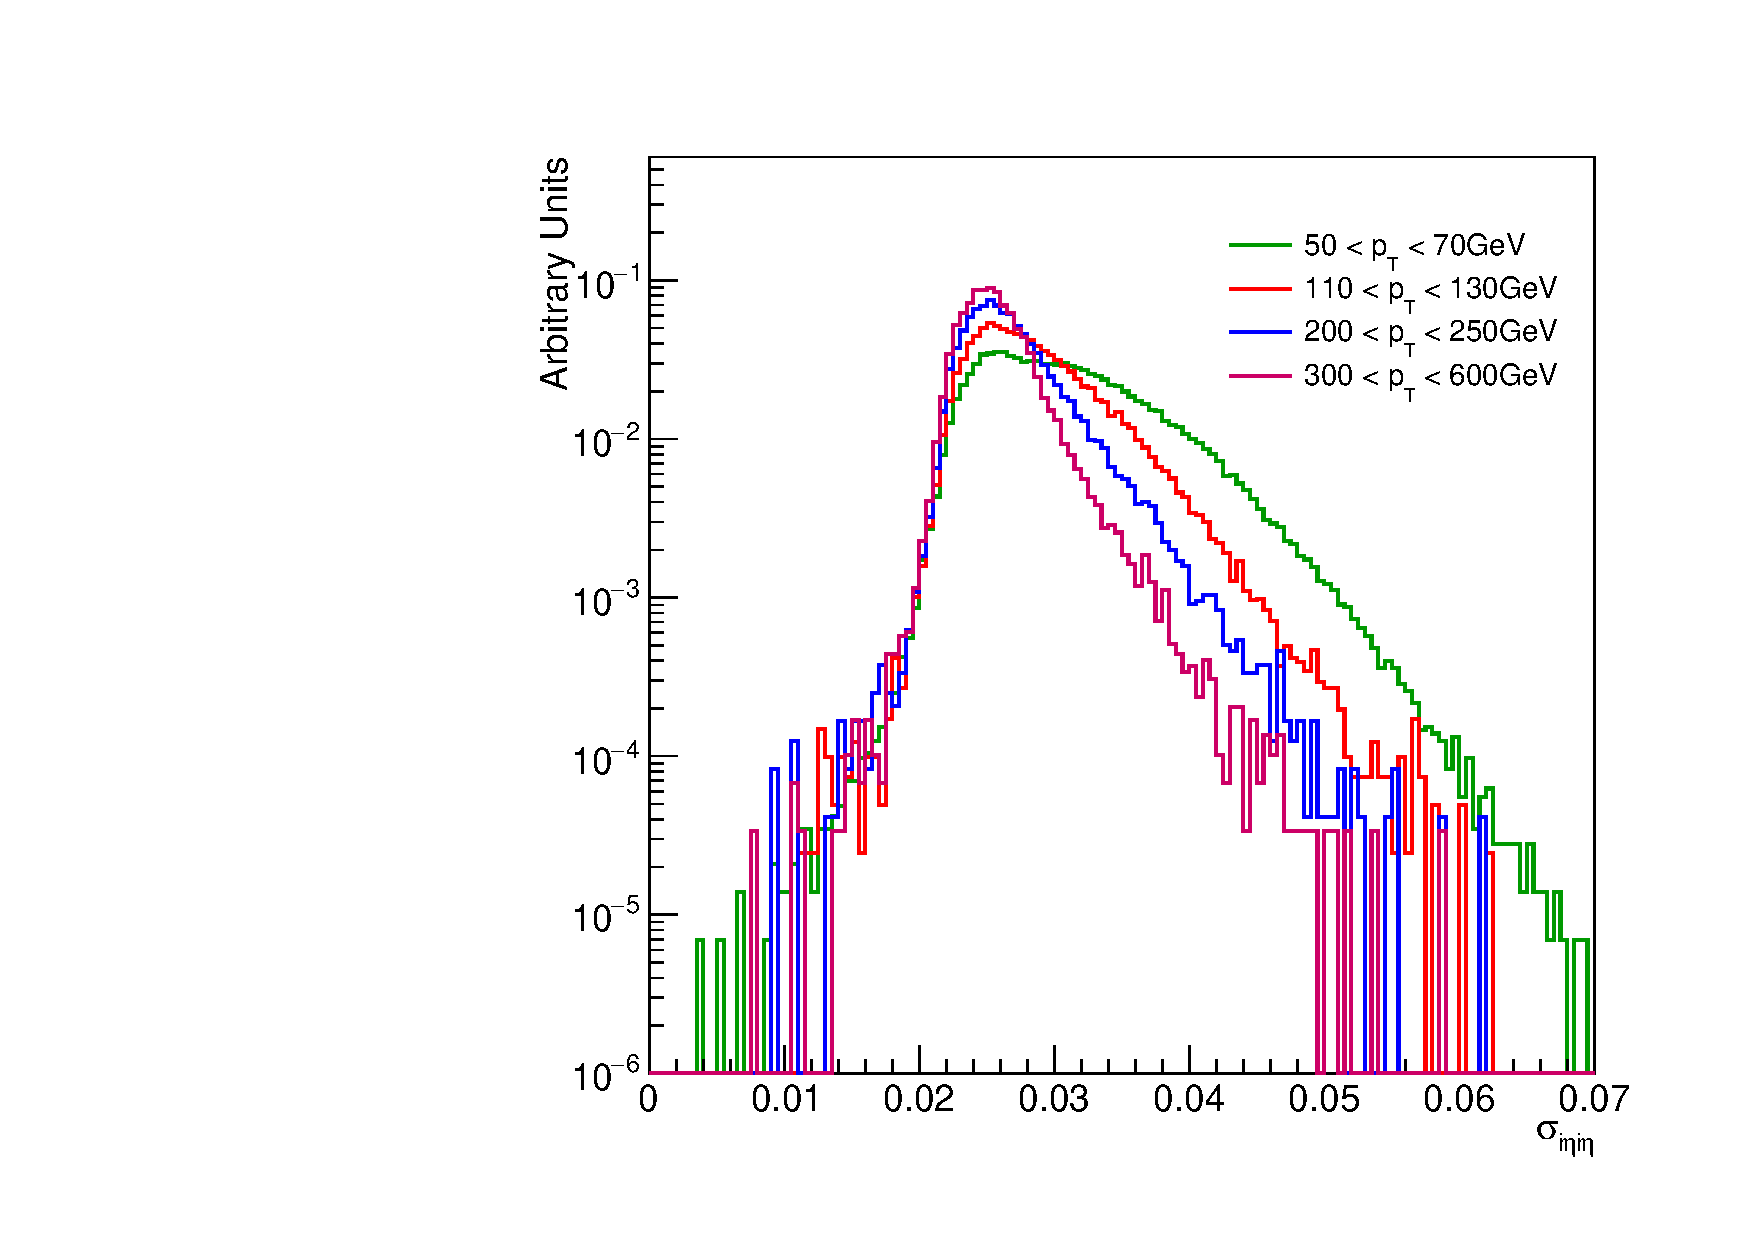
\includegraphics[width=0.49\textwidth]{fig/faketemplatecompEE_jetht_2018.pdf}
\label{fig:fake_templates}
\end{figure}

There is very little dependence of the template shape on the year. This is shown for the real template in Figure~\ref{fig:real_templates_by_year} for photons in each of the three calorimeter regions. Figure~\ref{fig:fake_templates_by_year} shows the same for the fake templates, separated by the data set in which they are derived. 

% % % generated by FakeRateAnalysis/python/plot_templates_by_year.py
\begin{figure}[!htbp]
\caption{Comparison of normalized real template shape among the three analysis years, for EB (left), EE1 ($1.566 < |\eta| < 2.033$)(center), and EE2 ($2.033 < \lvert \eta \rvert< 2.5$)(right).}
\centering
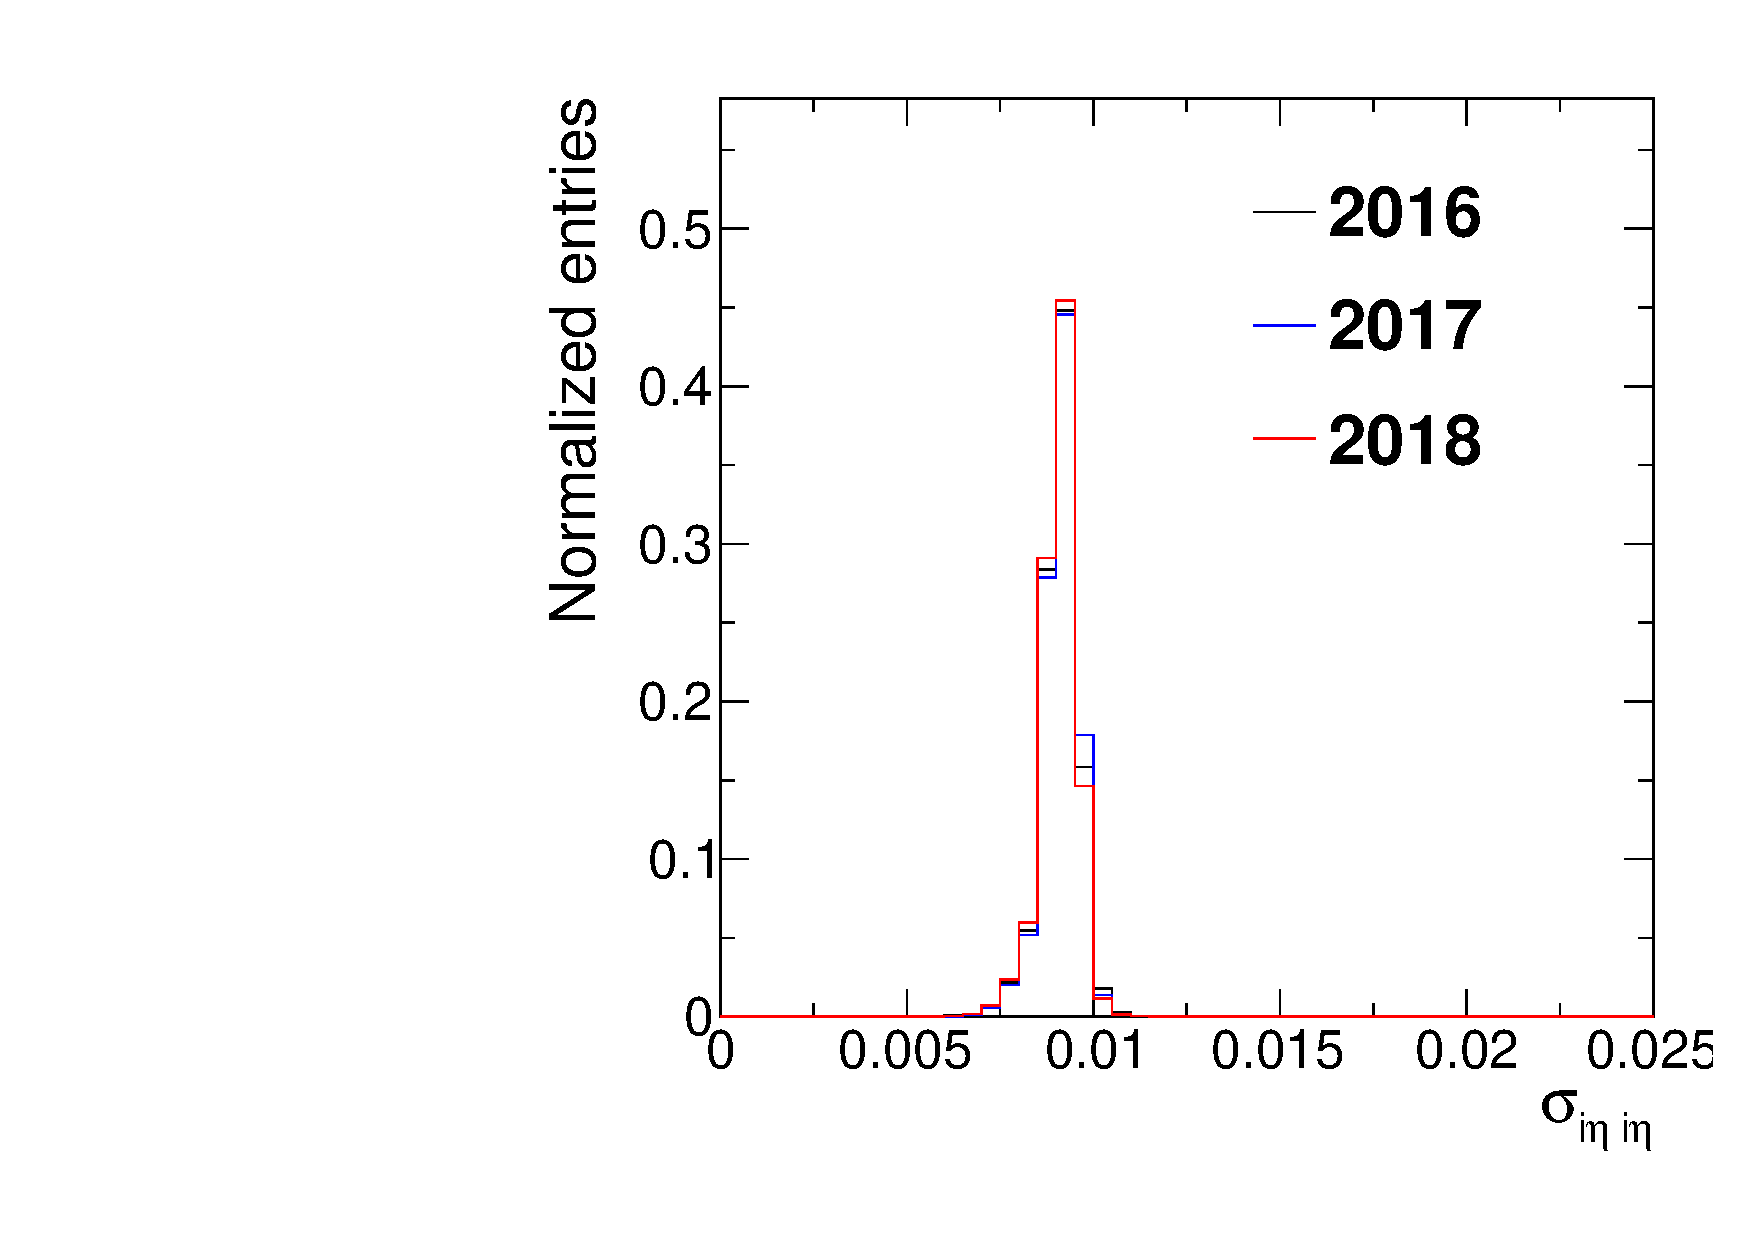
\includegraphics[width=0.3\textwidth]{fig/sieie_comparison_EB_diphoton_fake_rate_real_templates_all_GGJets_GJets_pt130To150_chIso5To10.pdf}
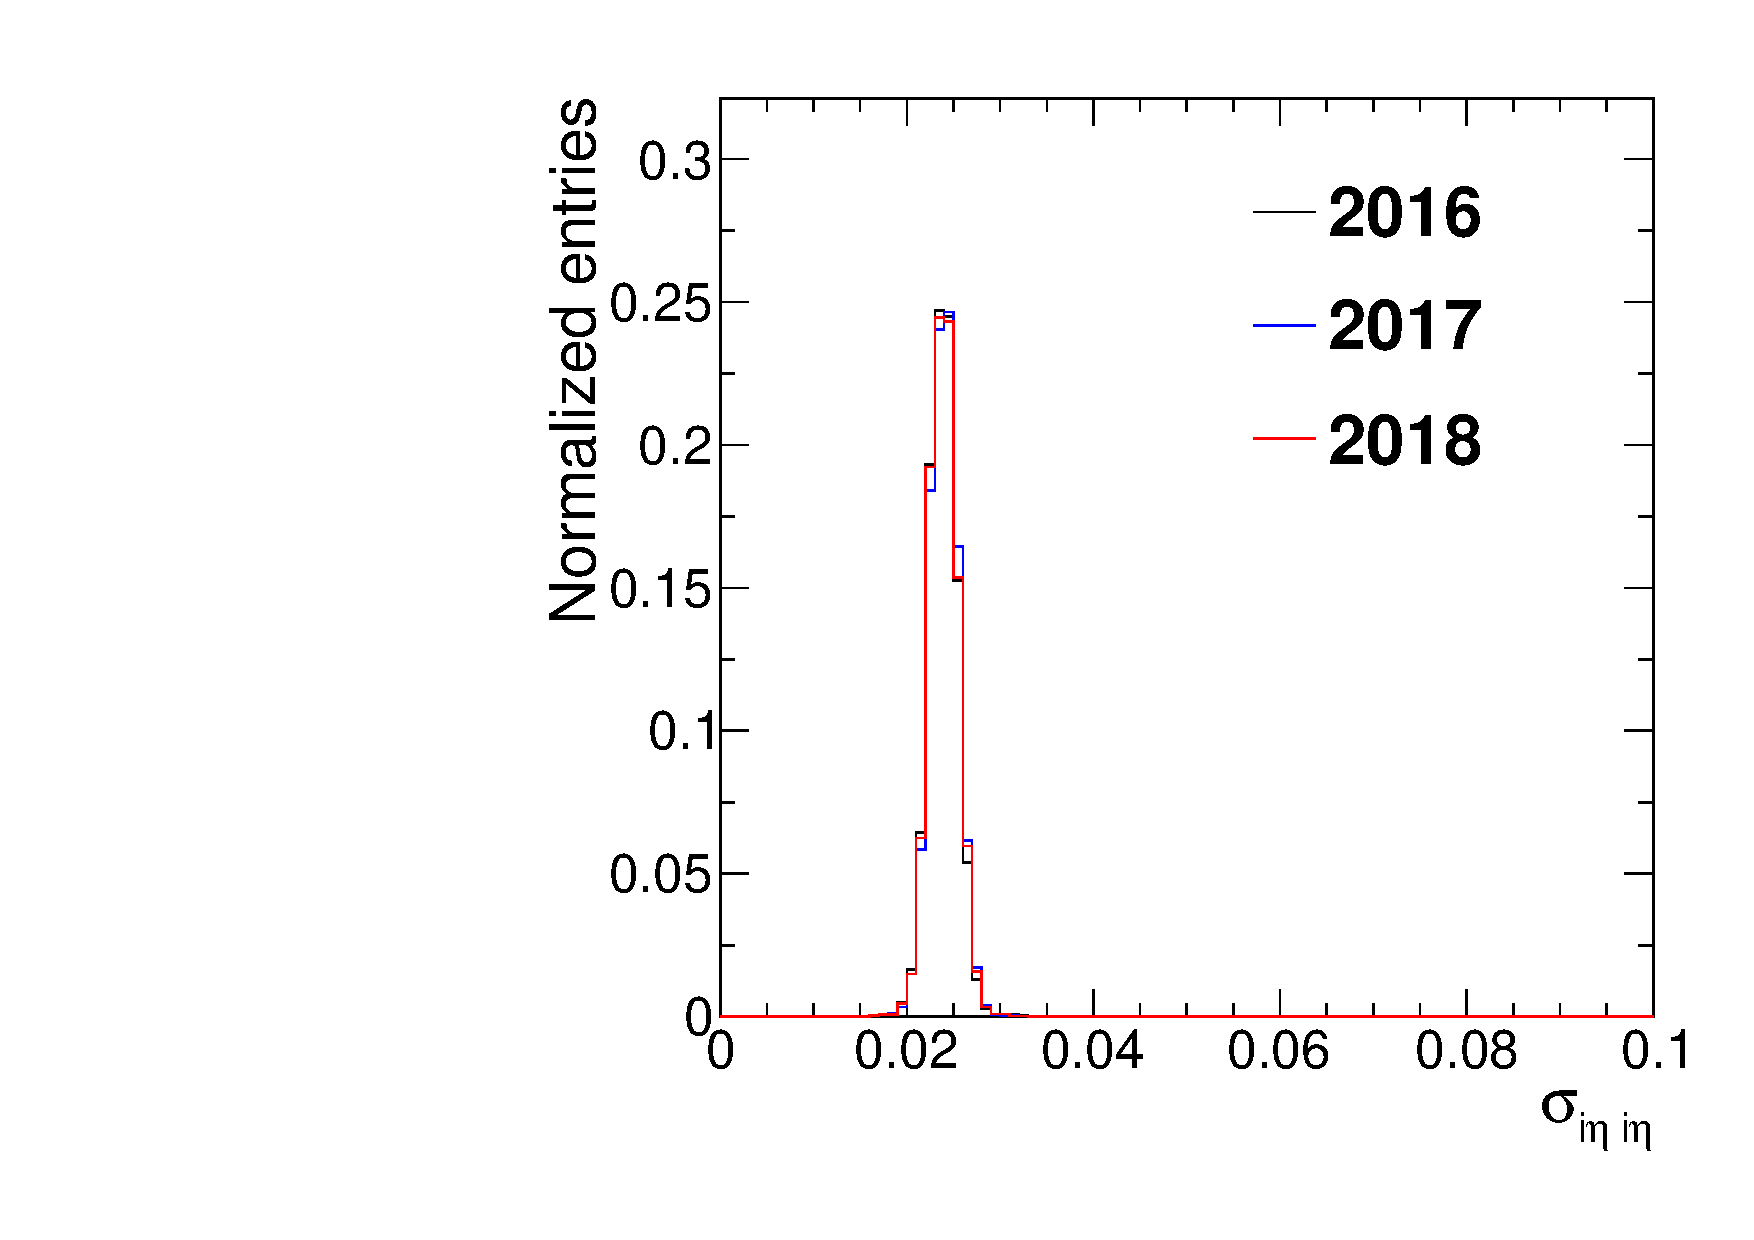
\includegraphics[width=0.3\textwidth]{fig/sieie_comparison_EE1_diphoton_fake_rate_real_templates_all_GGJets_GJets_pt130To150_chIso5To10.pdf}
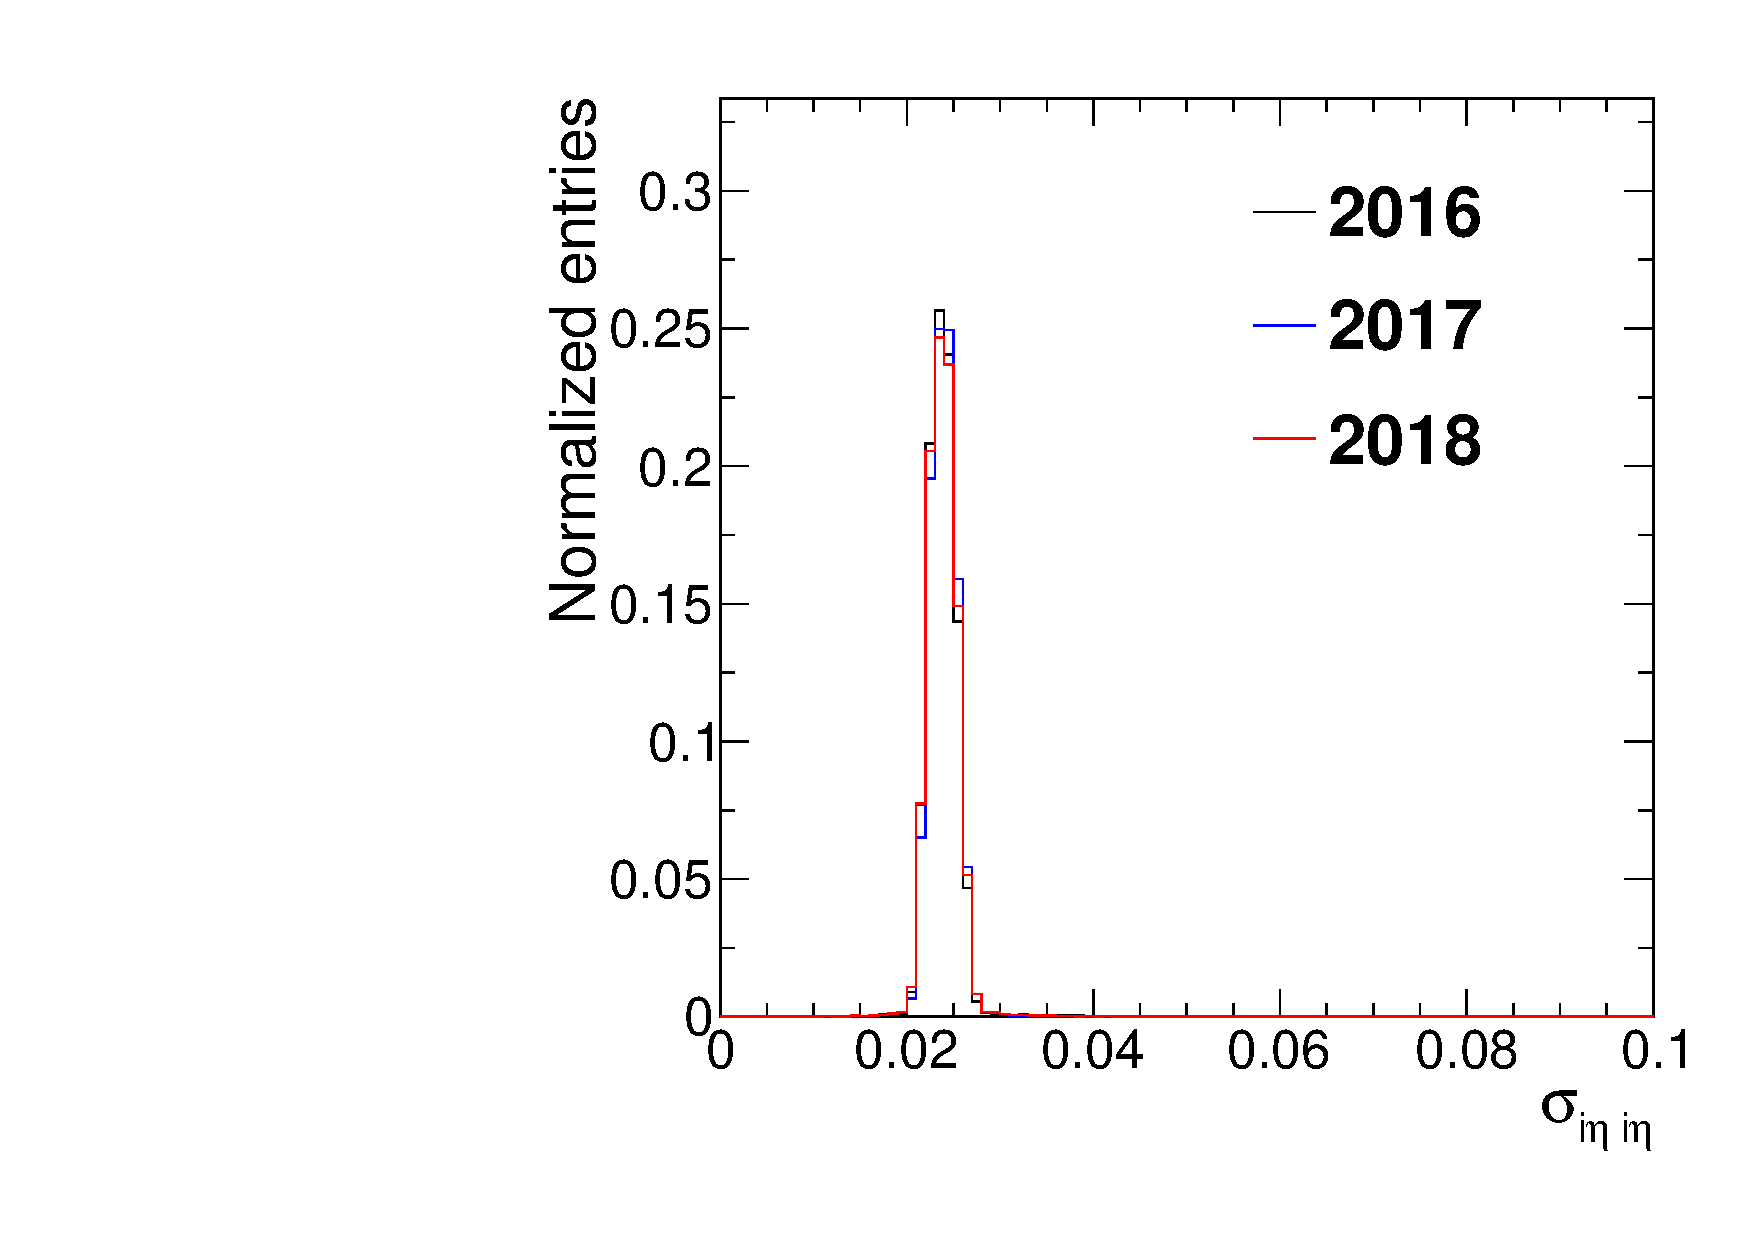
\includegraphics[width=0.3\textwidth]{fig/sieie_comparison_EE2_diphoton_fake_rate_real_templates_all_GGJets_GJets_pt130To150_chIso5To10.pdf}
\label{fig:real_templates_by_year}
\end{figure}

% % % generated by FakeRateAnalysis/python/plot_templates_by_year.py
\begin{figure}[!htbp]
\caption{Comparison of normalized fake template shape among the three analysis years, for EB (left), EE1 ($1.566 < |\eta| < 2.033$)(center), and EE2 ($2.033 < \lvert \eta \rvert< 2.5$)(right). The top (bottom) row shows the templates derived from the \texttt{JetHT} (\texttt{DoubleMuon}) dataset.}
\centering
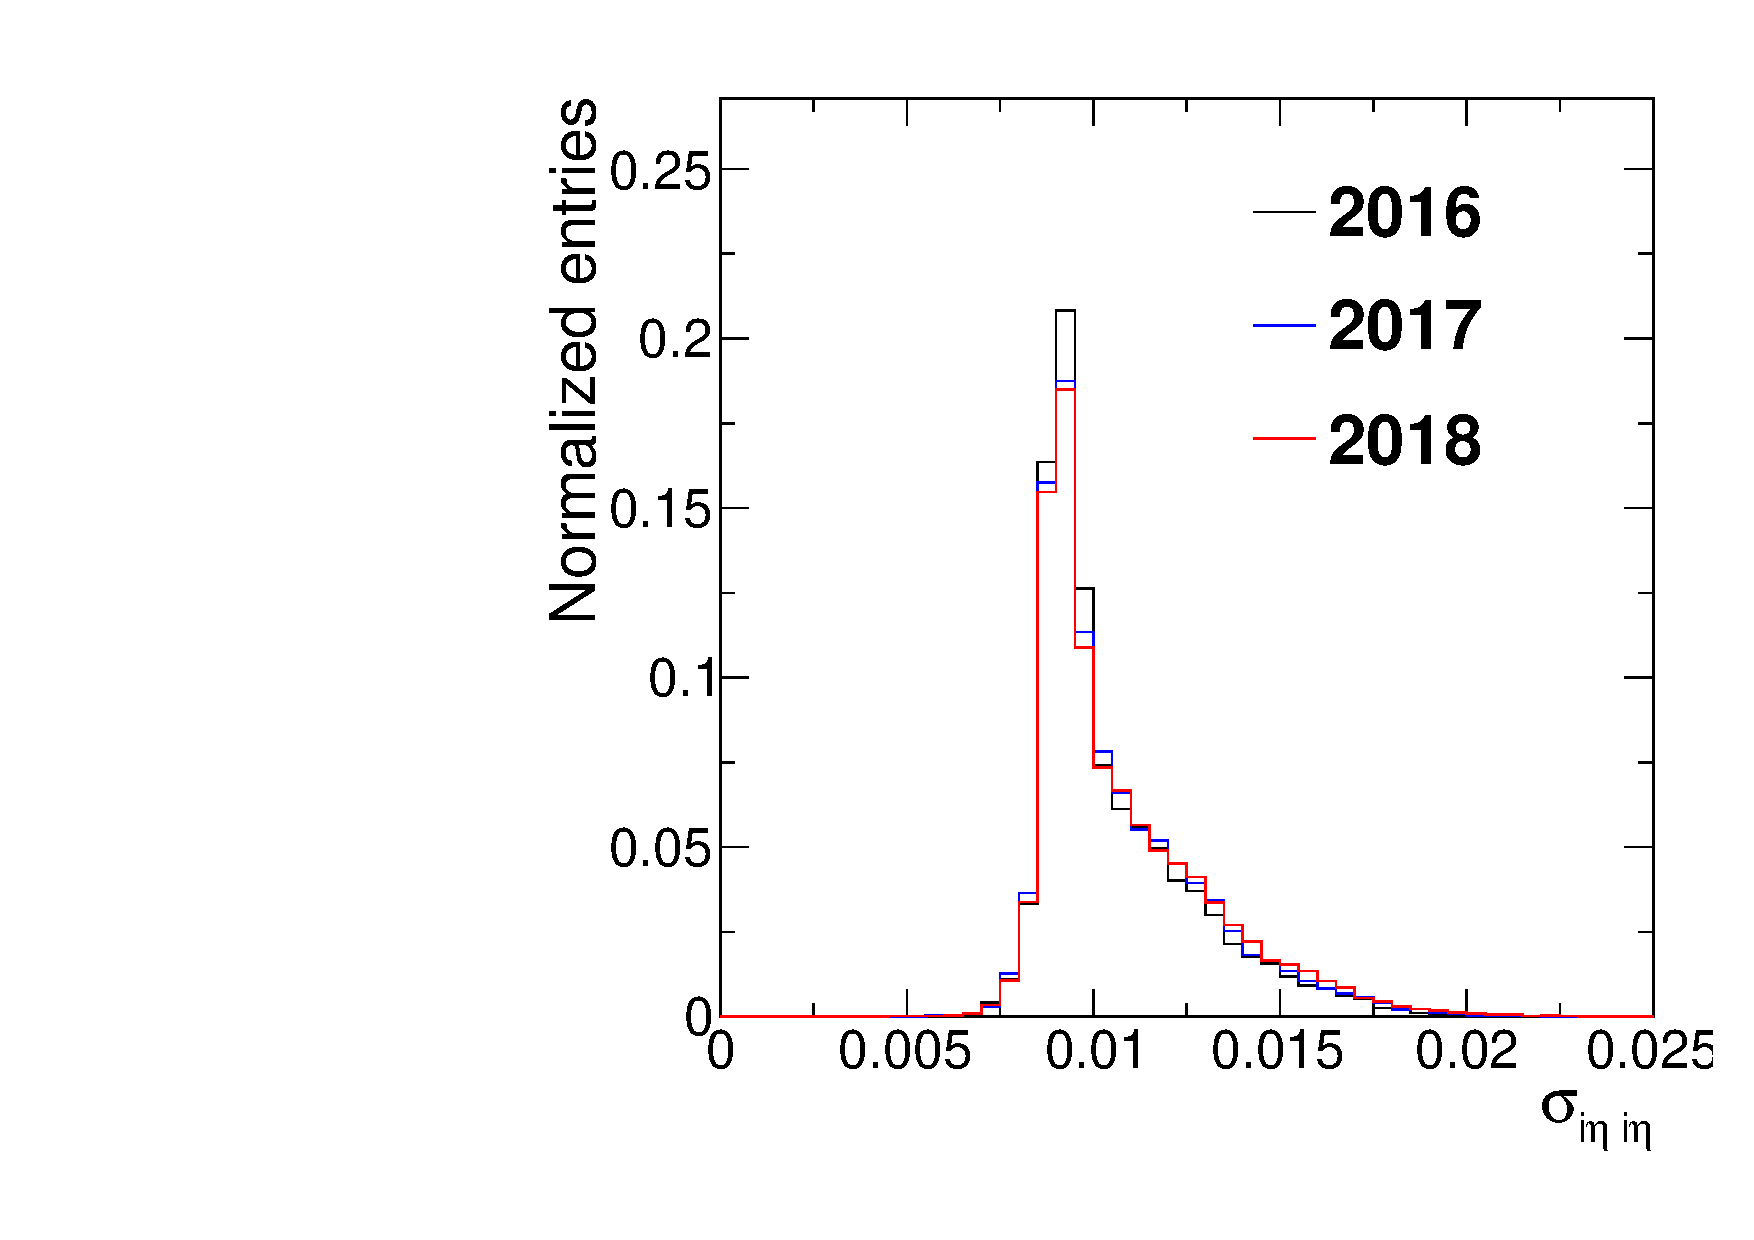
\includegraphics[width=0.3\textwidth]{fig/sieie_comparison_EB_jetht_pt130To150_chIso5To10.pdf}
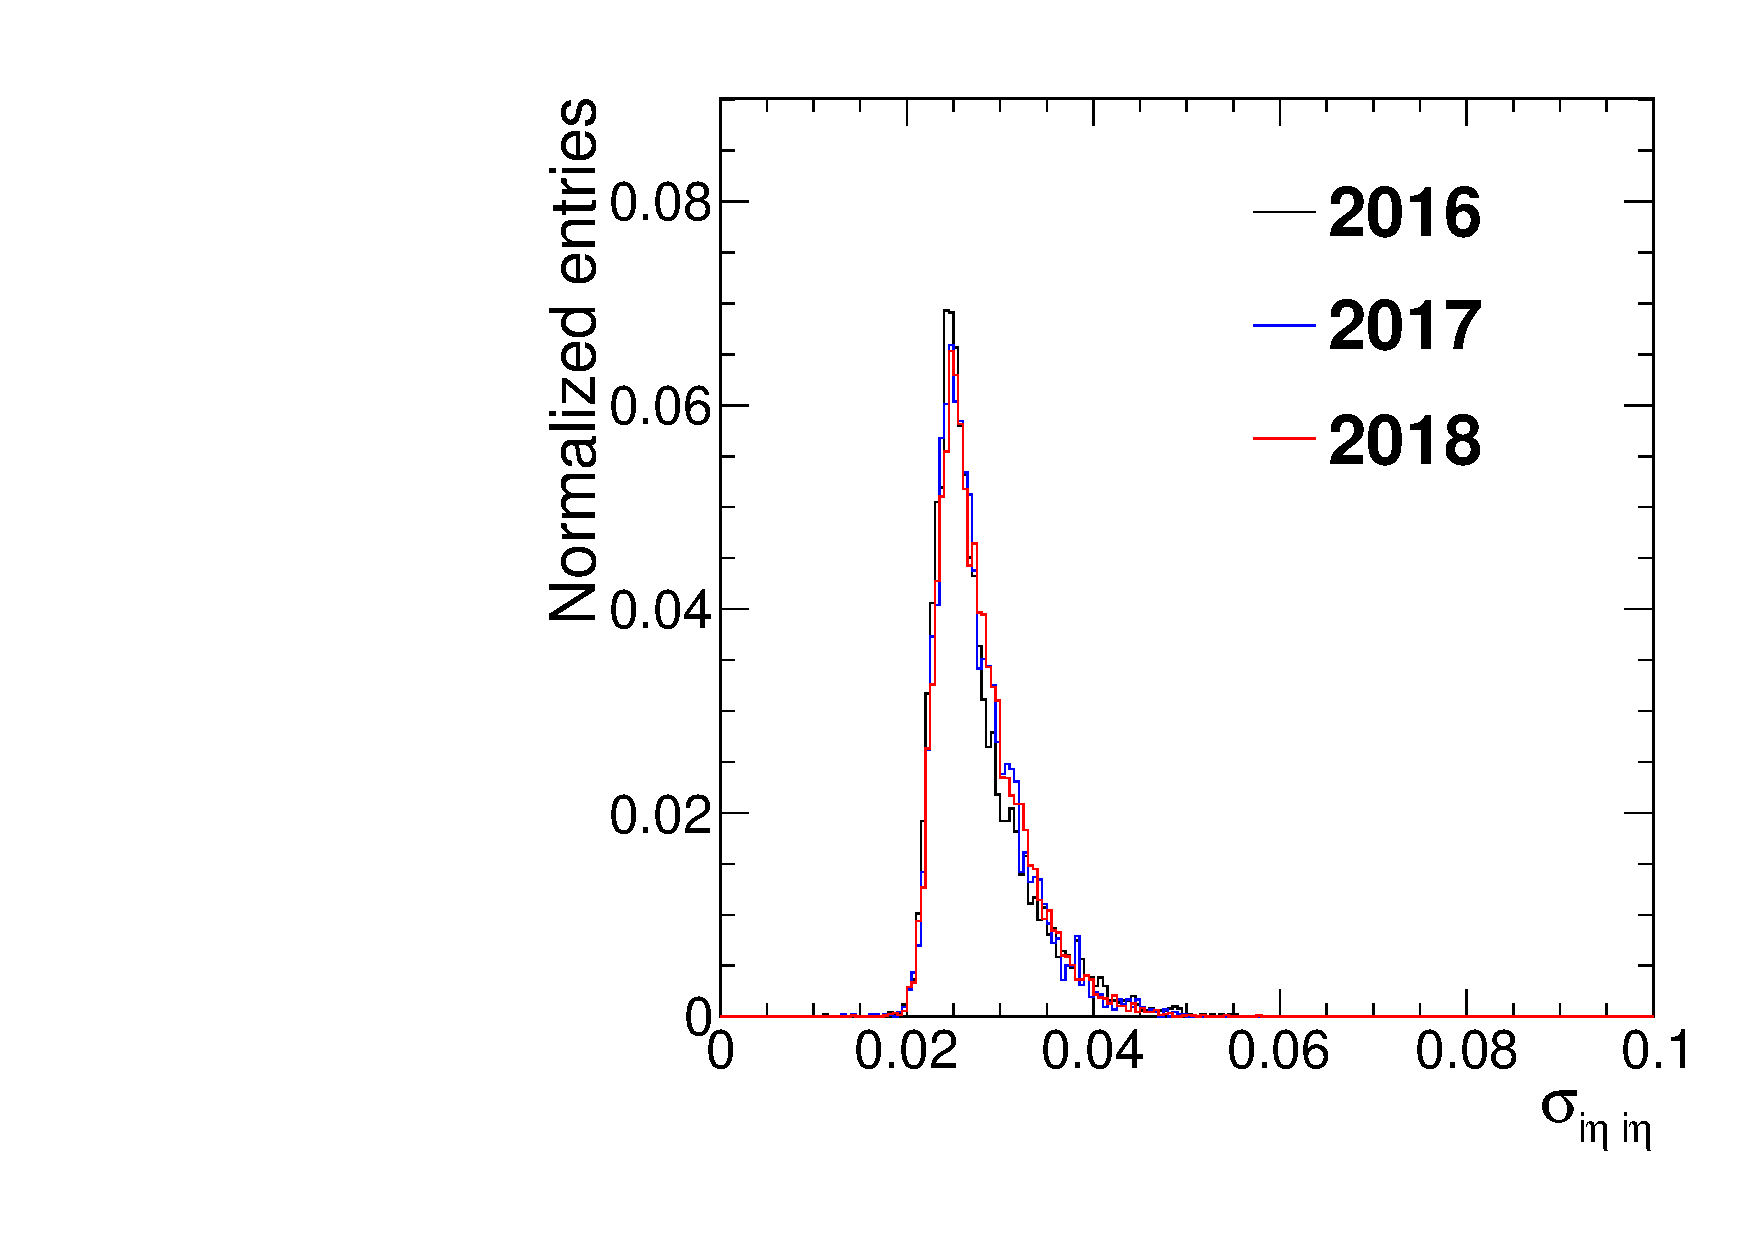
\includegraphics[width=0.3\textwidth]{fig/sieie_comparison_EE1_jetht_pt130To150_chIso5To10.pdf}
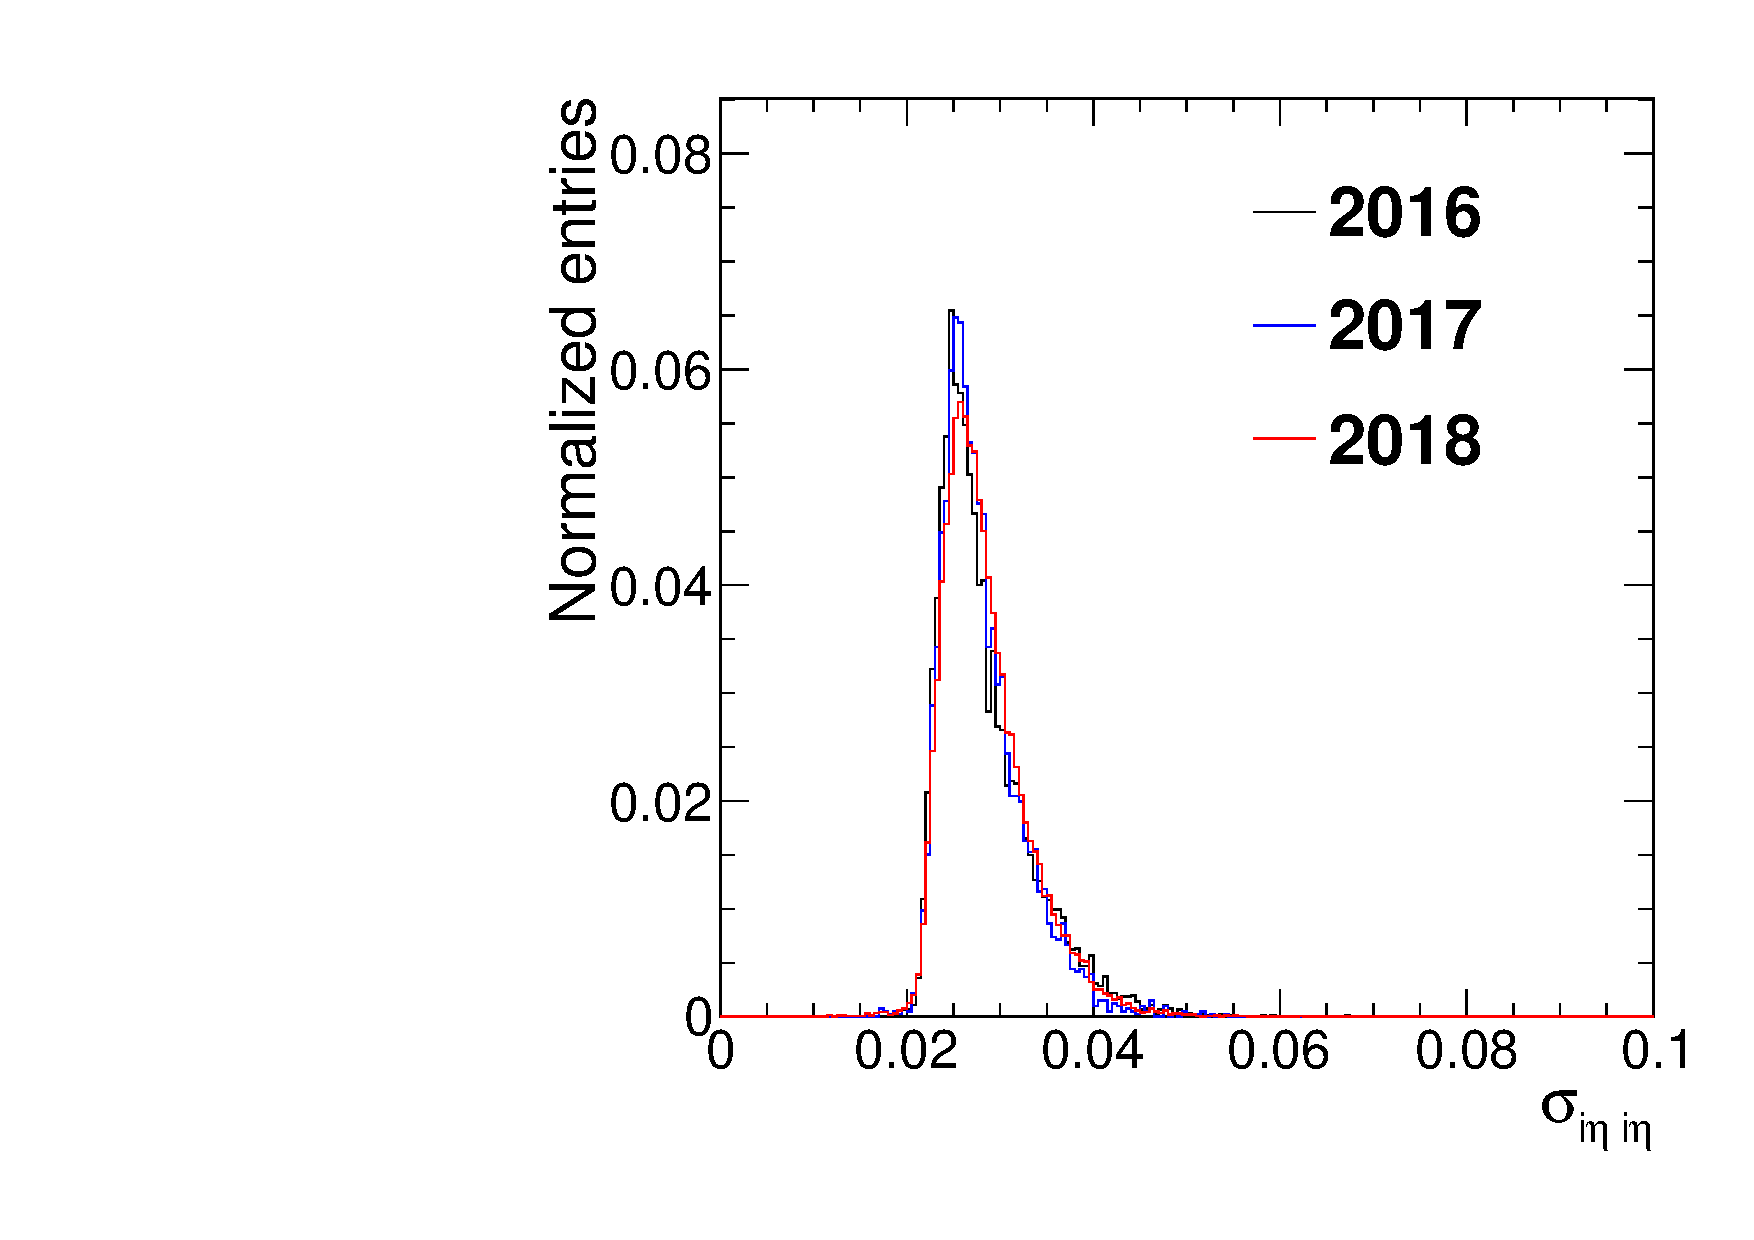
\includegraphics[width=0.3\textwidth]{fig/sieie_comparison_EE2_jetht_pt130To150_chIso5To10.pdf}\\
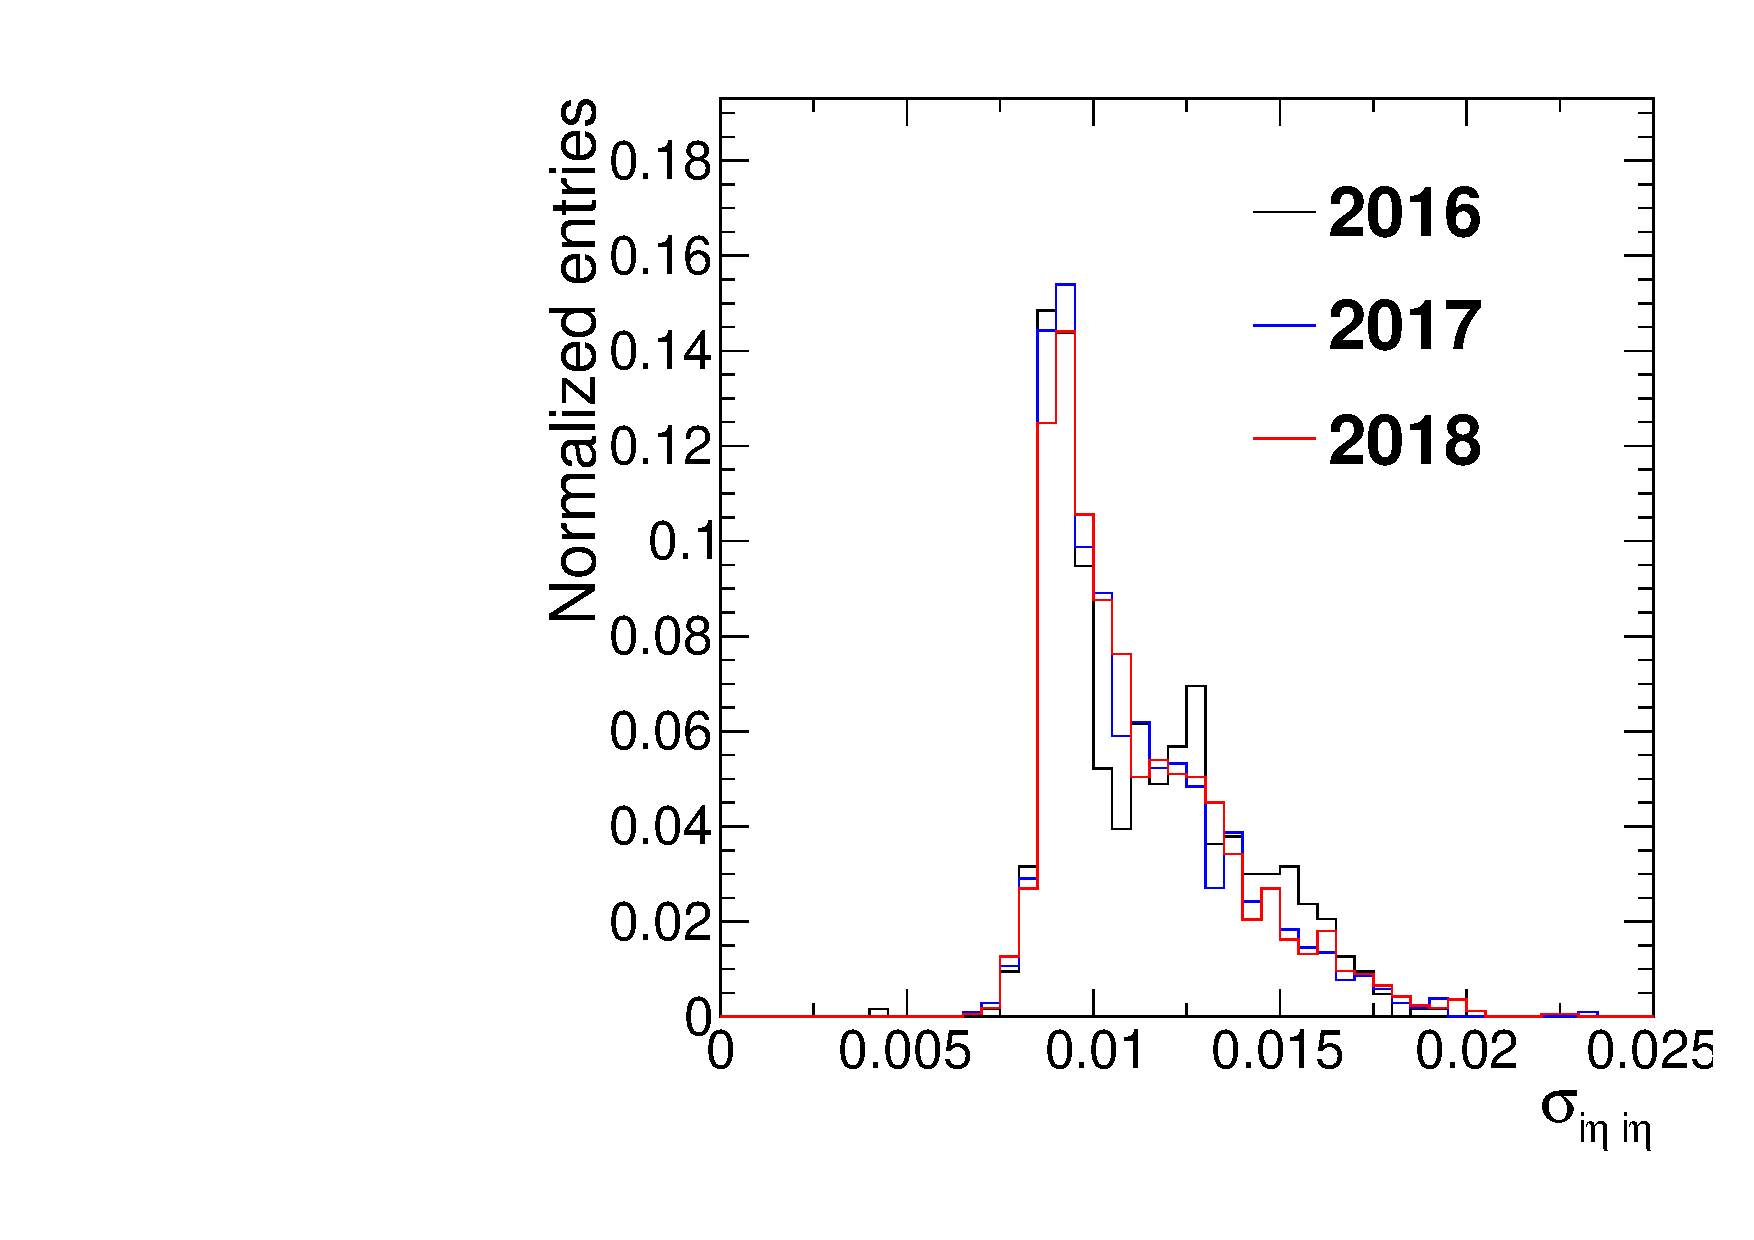
\includegraphics[width=0.3\textwidth]{fig/sieie_comparison_EB_doublemuon_pt130To150_chIso5To10.pdf}
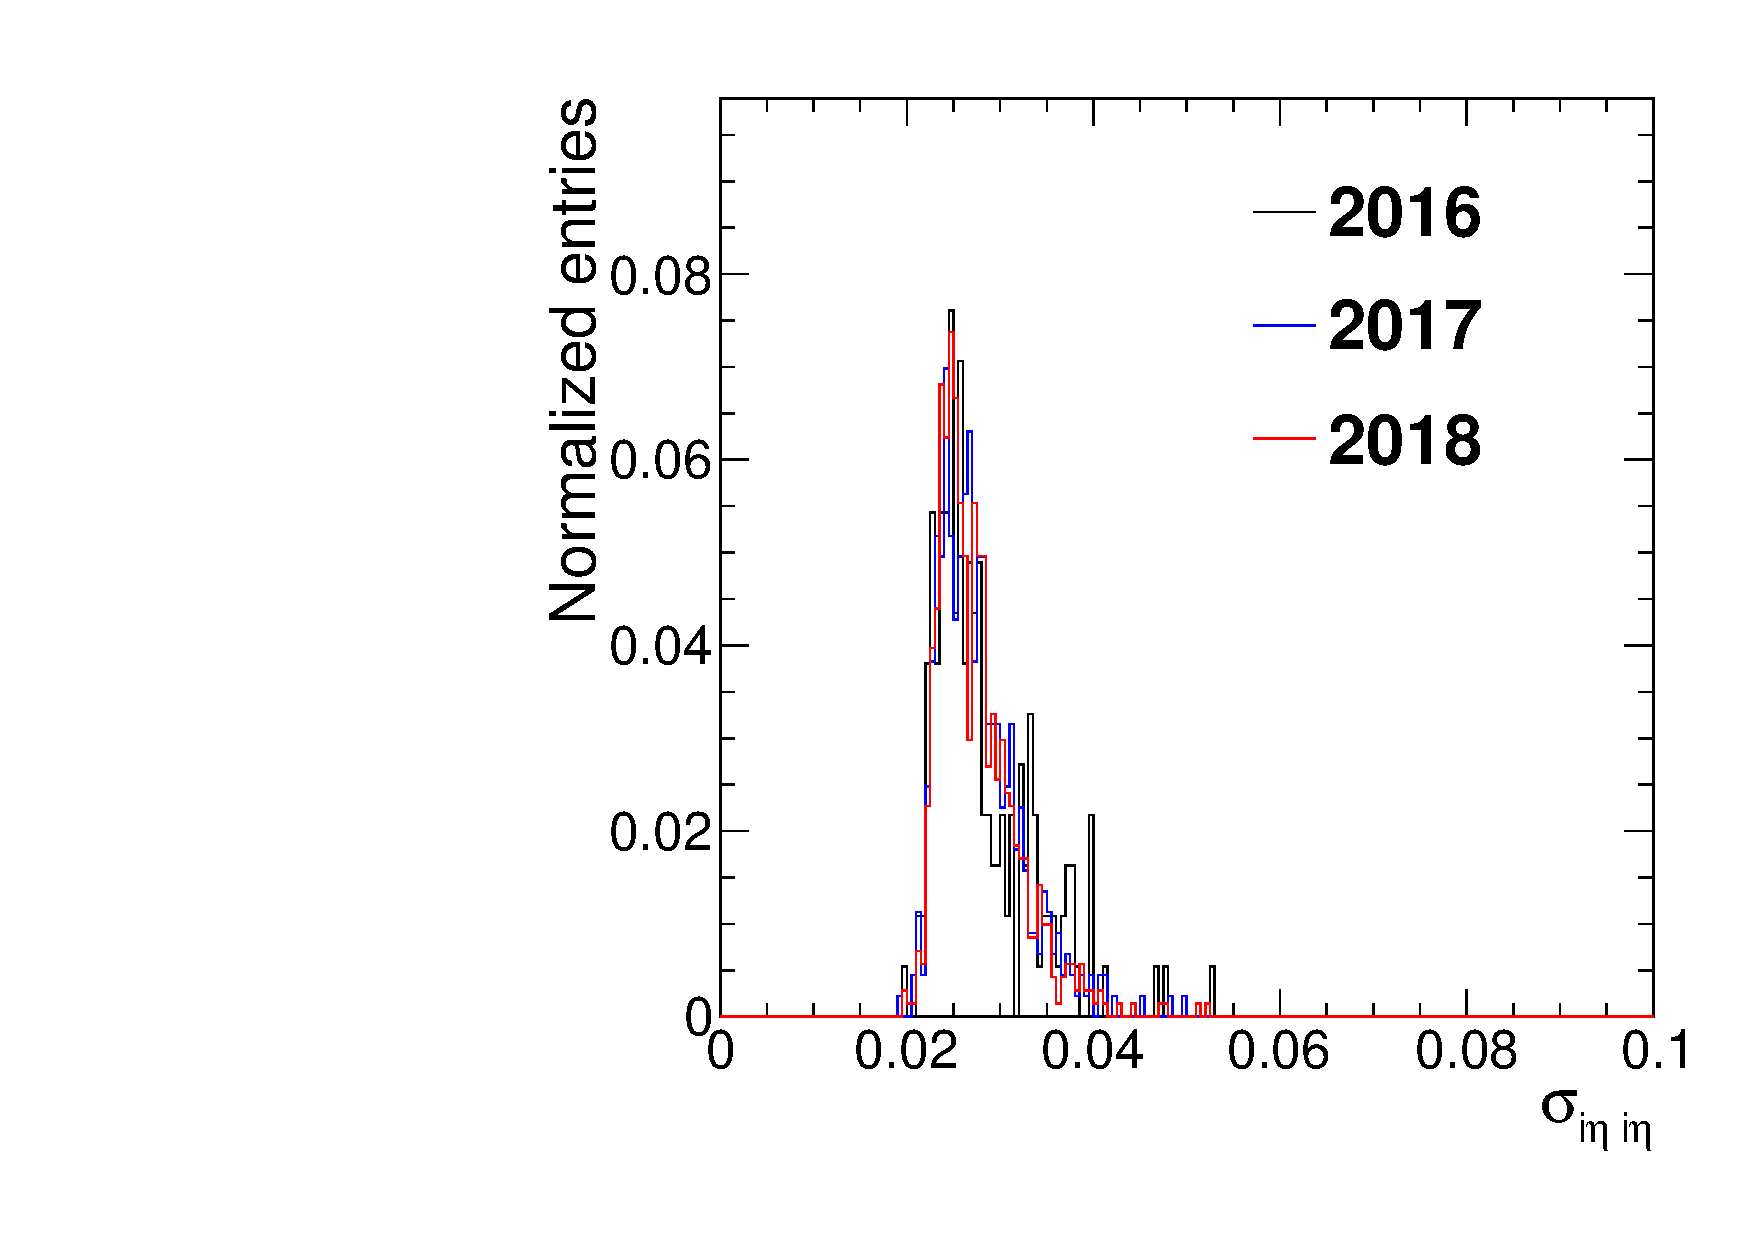
\includegraphics[width=0.3\textwidth]{fig/sieie_comparison_EE1_doublemuon_pt130To150_chIso5To10.pdf}
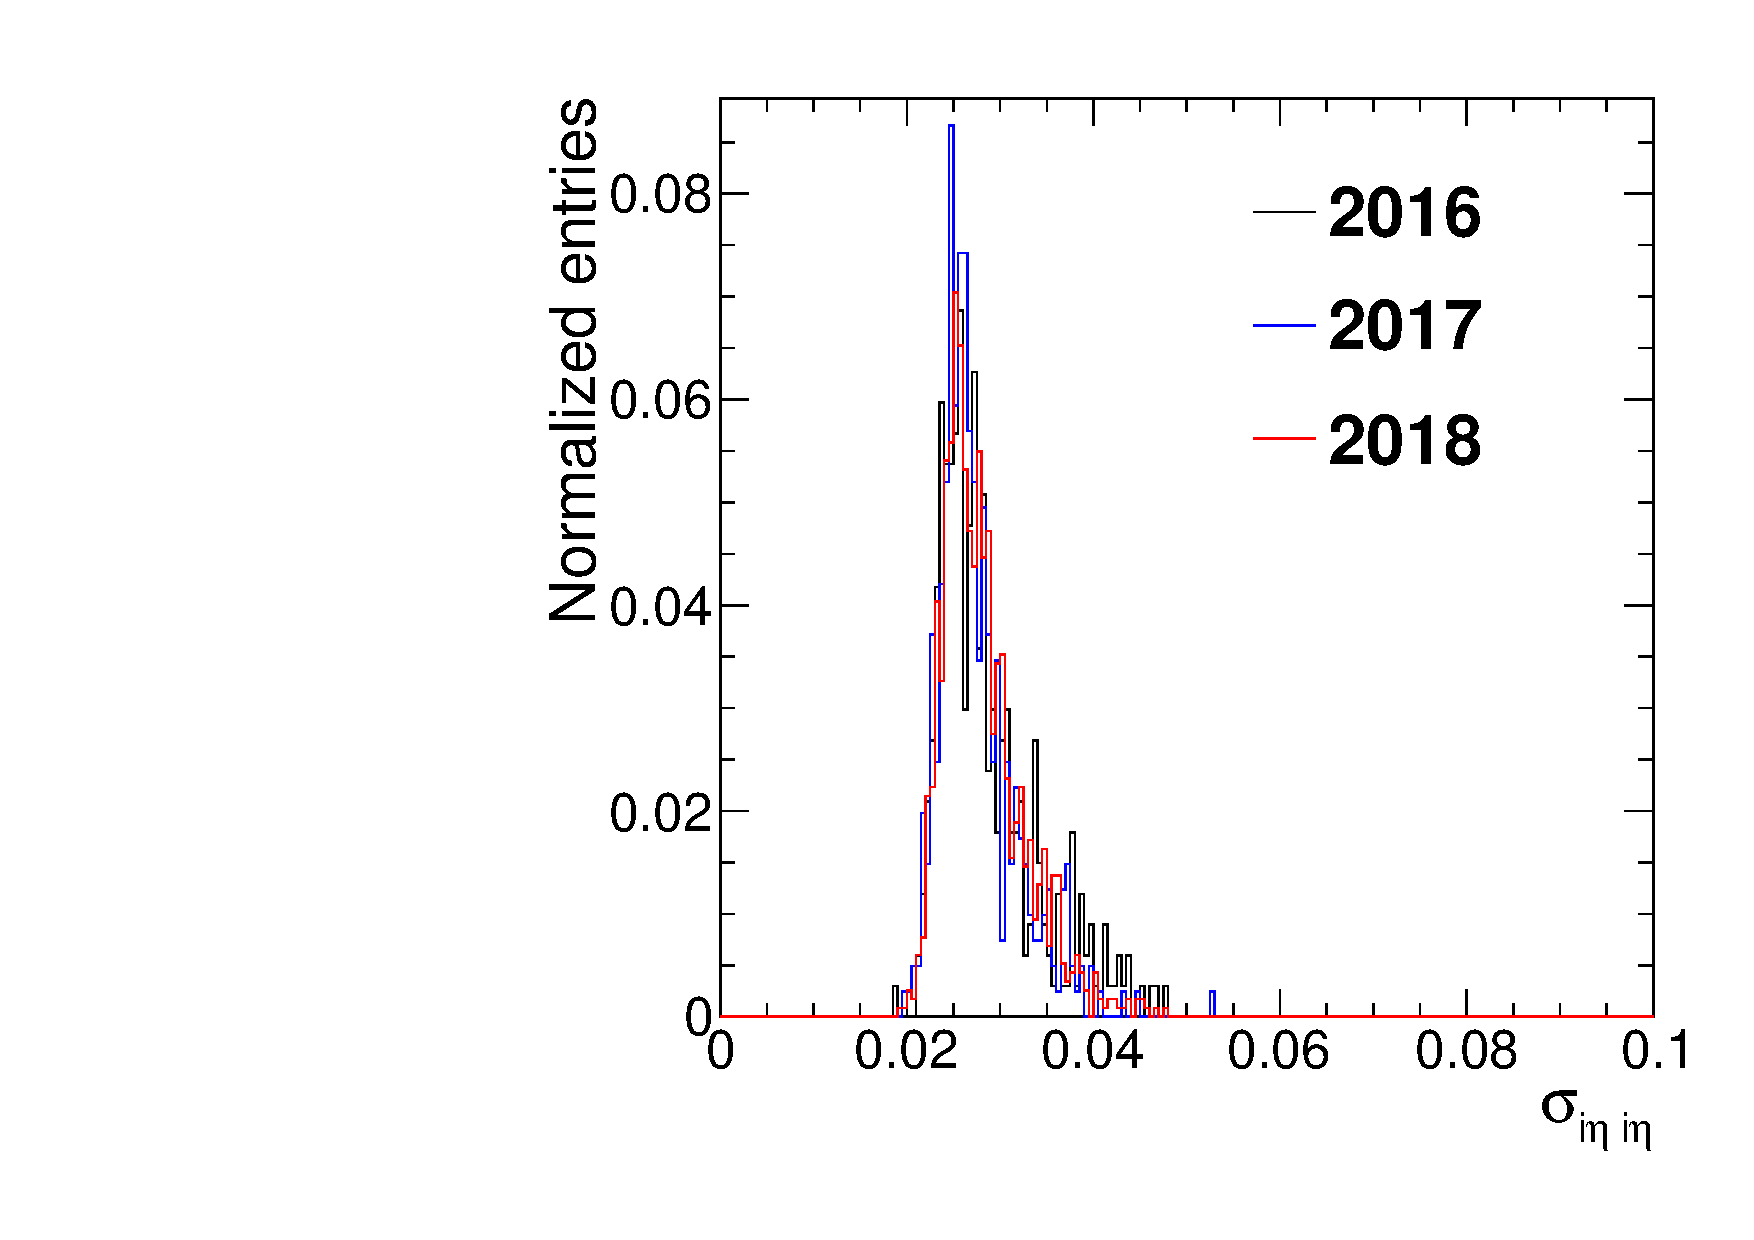
\includegraphics[width=0.3\textwidth]{fig/sieie_comparison_EE2_doublemuon_pt130To150_chIso5To10.pdf}
\label{fig:fake_templates_by_year}
\end{figure}

% % %%FIXME: illustration of templates and fit!
An illustration of the template fit for a given \pt bin is shown in Figure~\ref{fig:templatefit}. Real photons are primarily found near the peak for the \sieie template variable, while the fake photons generally populate the broad tail at large \sieie values. This indicates a broader shower-shape in ECAL, arising from the presence of more than one photon in the shower from neutral meson decays. The overall scale factors for the real and fake templates serve as the only two free parameters for the fit. After fitting, the post-fit fake template is integrated from $\sieie=0$ up to the appropriate cut value from Table~\ref{table:highptid} to give the estimated number of fake-photons-from-jets in the sample. This number serves as the value for the \emph{numerator} in our fake rate for the particular \pt bin. 

% % % generated by fakeRateCalculation.exe
\begin{figure}[!htbp]
\caption{A representative template fit extracted from the 2018 \texttt{JetHT} data set using photon objects from the ECAL barrel in the $130<\pt<150\GeV$ range, in linear (left) and log scale (right) for the y-axis.}
\centering
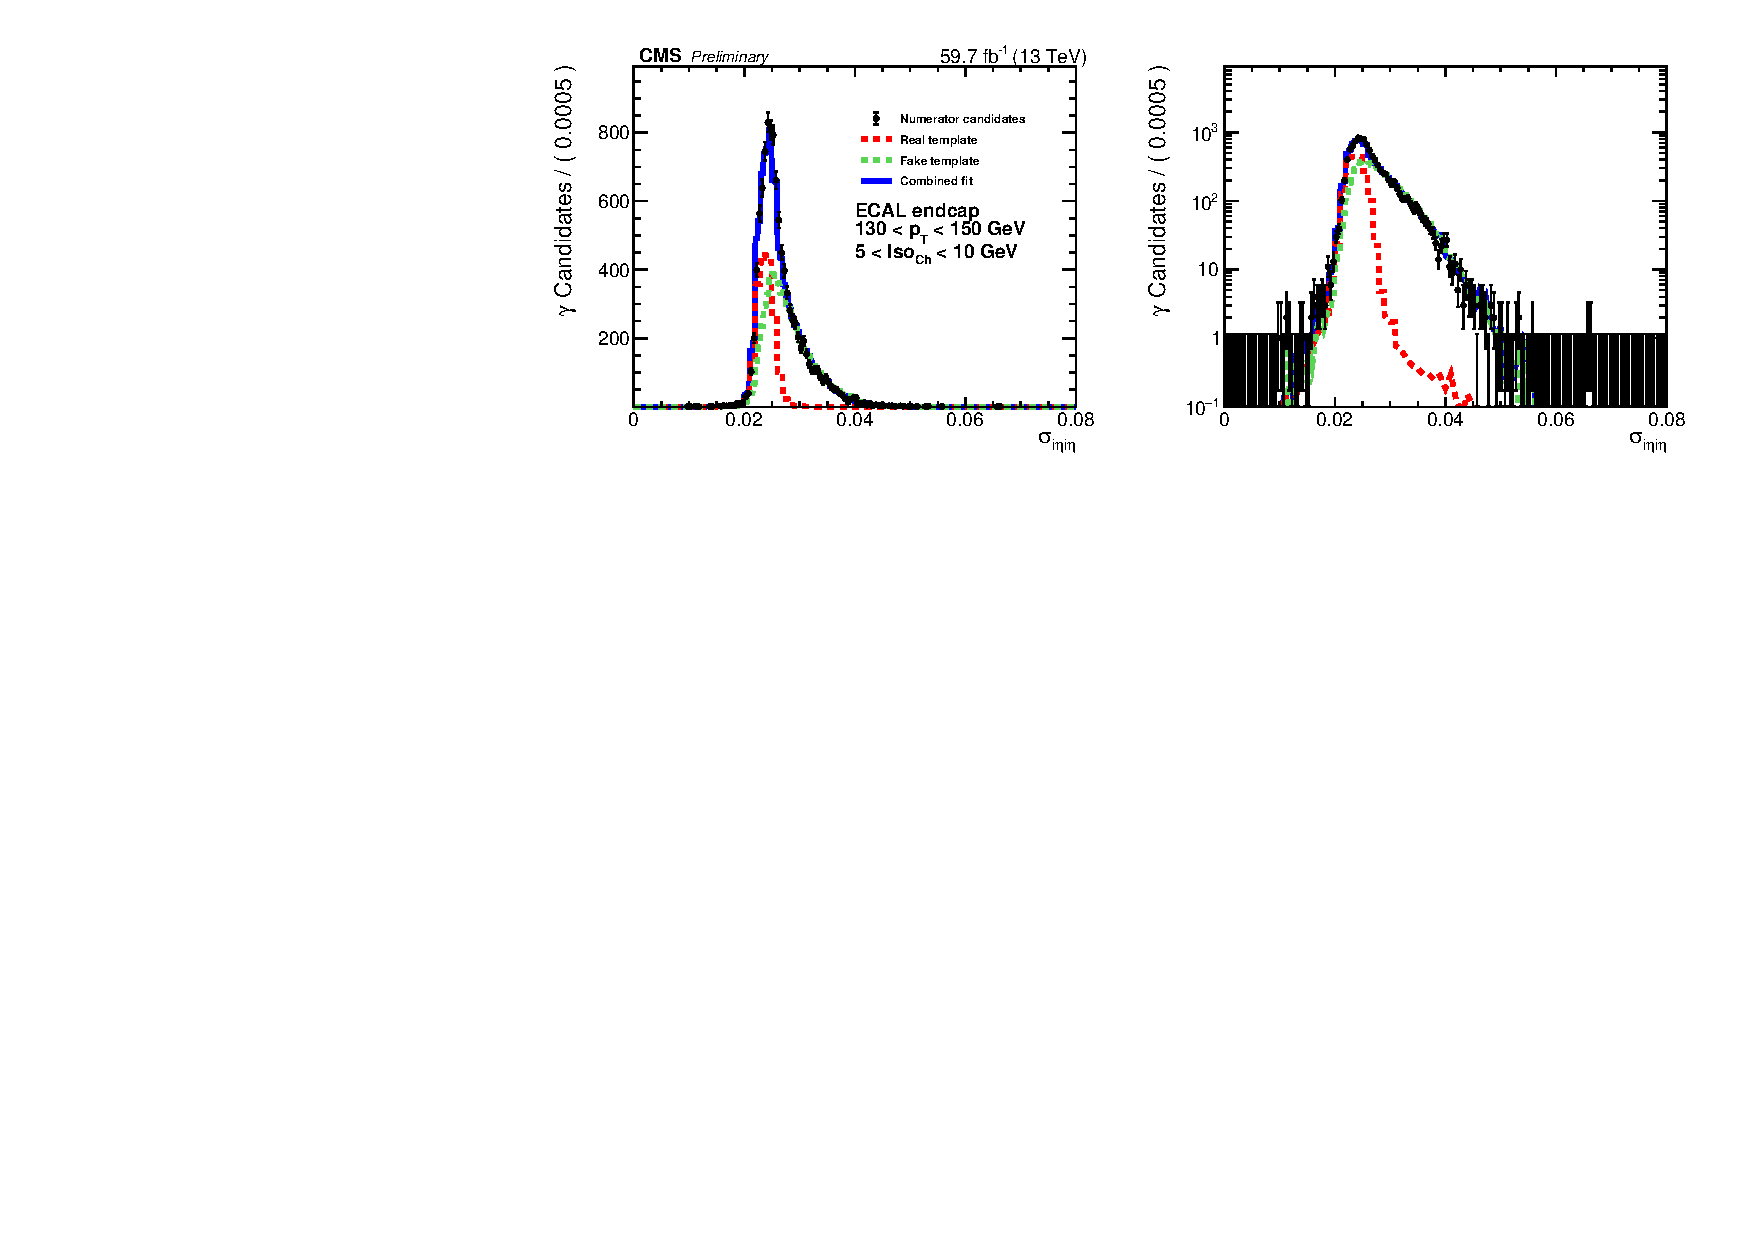
\includegraphics[scale=0.80]{fig/fakeRatePlot_jetht_2018_EE_pT130To150_chIso5To10.pdf}
\label{fig:templatefit}
\end{figure}

\subsection{Fake Rate Denominator}

We definee the denominator of the fake rate as a count of the number of objects passing our denominator definition in each $\pt$ bin. While this definition is arbitrary, the denominator objects obtained from the \texttt{JetHT} sample and the \texttt{DoubleEG} samples must be similar with this choice of definition which is defined as follows:
\begin{enumerate}
    \item Denominator object must \emph{FAIL} one of the high-\pt ID cuts
    \item Must \emph{PASS} the conversion-safe electron veto (CSEV)
    \item Both \chiso and \corphoiso must be $< 0.2$ times the object's \pt
    \item Cone-based H/E $< 0.1$ 
    \item $\RNINE>0.8$ to match the photon preselection cut.
\end{enumerate}~ label{denom_definition}

The first criteria requires that the denominator object fails at least one of the Photon ID cuts. This ensures that the denominator sample is orthogonal to the numerator, and is not contaminated by real photons. Additionally, the object must pass the conversion-safe electron veto variable which is a variable designed to reject direct electrons but not electrons that originate from photon conversions. To ensure that the denominator objects are still photon-like-jets, that is they are still reasonably isolated, we require that the isolation variables are not too large ($<20$\% maximum). This is important since we are reweighting the denominator by the fake rate to estimate our fake prediction. The cone-based H/E cut is used in the photon ID at HLT level while the tower-based Had/EM is the more typical offline variable used in our photon ID. Since we are selecting from data, we use the cone-based H/E cut. 

% The Conversion-safe electron veto is designed as a variable that rejects direct electrons and not electrons that might come from photon conversions. This veto requires that a photon cluster in the ECAL is not matched to a reconstructed conversion vertex, and a hit in the inner layer of the pixel detector associated with a charged-particle track indicating a direct and real electron~\cite{CMS:2015myp}. 

%%actual fake rate extracted
\subsection{Extracting the Fake Rate}

The fake rate is just the ratio of the numerator and denominator which we have counted using the procedure described above. The fake rate is primarily a function of \pt and is determined for EB and EE separately. The EE is further split into two bins, which we show later in Sec.~\ref{sec:closure_test} to be an improvement in our fake prediction for the $\eta$ distributions. The fake rates are also dependent on the number of selected primary vertices. This is shown in Figure~\ref{fig:frpileup_EB}, Figure~\ref{fig:frpileup_EE1}, and Figure~\ref{fig:frpileup_EE2} for EB, EE1 and EE2, respectively. EE1 covers the region $1.566 < |\eta| < 2.033$ while EE2 covers $2.033 < \lvert \eta \rvert< 2.5$. We take the average of the fake rates derived from the \texttt{JetHT} and \texttt{DoubleMuon} data sets. As a consequence of the lower statistics in the \texttt{DoubleMuon} dataset, the fake rate derivation have a different \pt binning. We apply the fake rate separately for each of the two data sets at the given \pt, then the two fake rates are averaged. We chose ranges for comparison that have a roughly uniform level of statistics between them.

% generated by compare_pv.exe
\begin{figure}[!htbp]
\caption{A comparison of the fake rate in EB measured as a function of the number of selected primary vertices (nPV) in the event using the \texttt{JetHT} data set (top) and \texttt{DoubleMuon} data set (bottom). The fake rates are determined separately for 2016 at the (left), 2017 (center), and 2018 (right).}
\centering
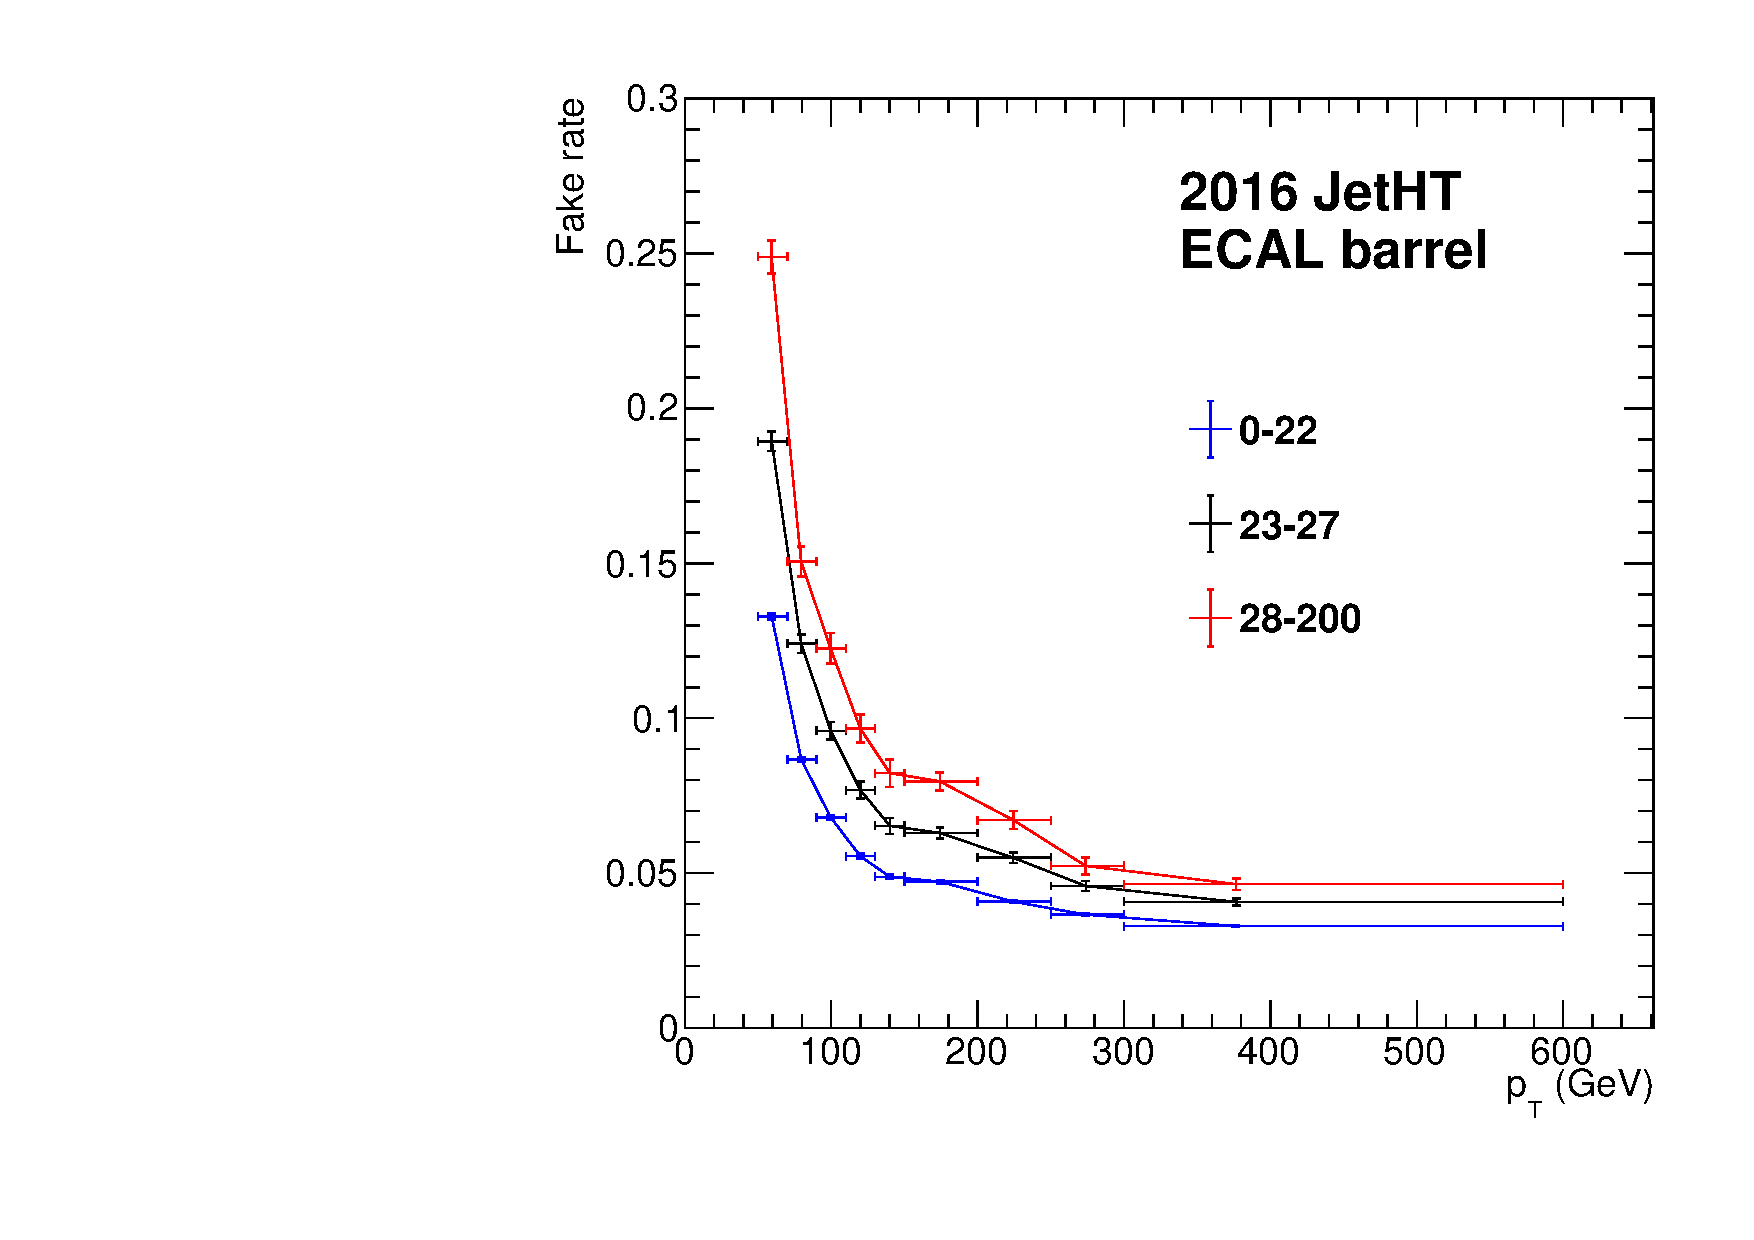
\includegraphics[width=0.3\textwidth]{fig/compare_pv_EB_2016_jetht.pdf}
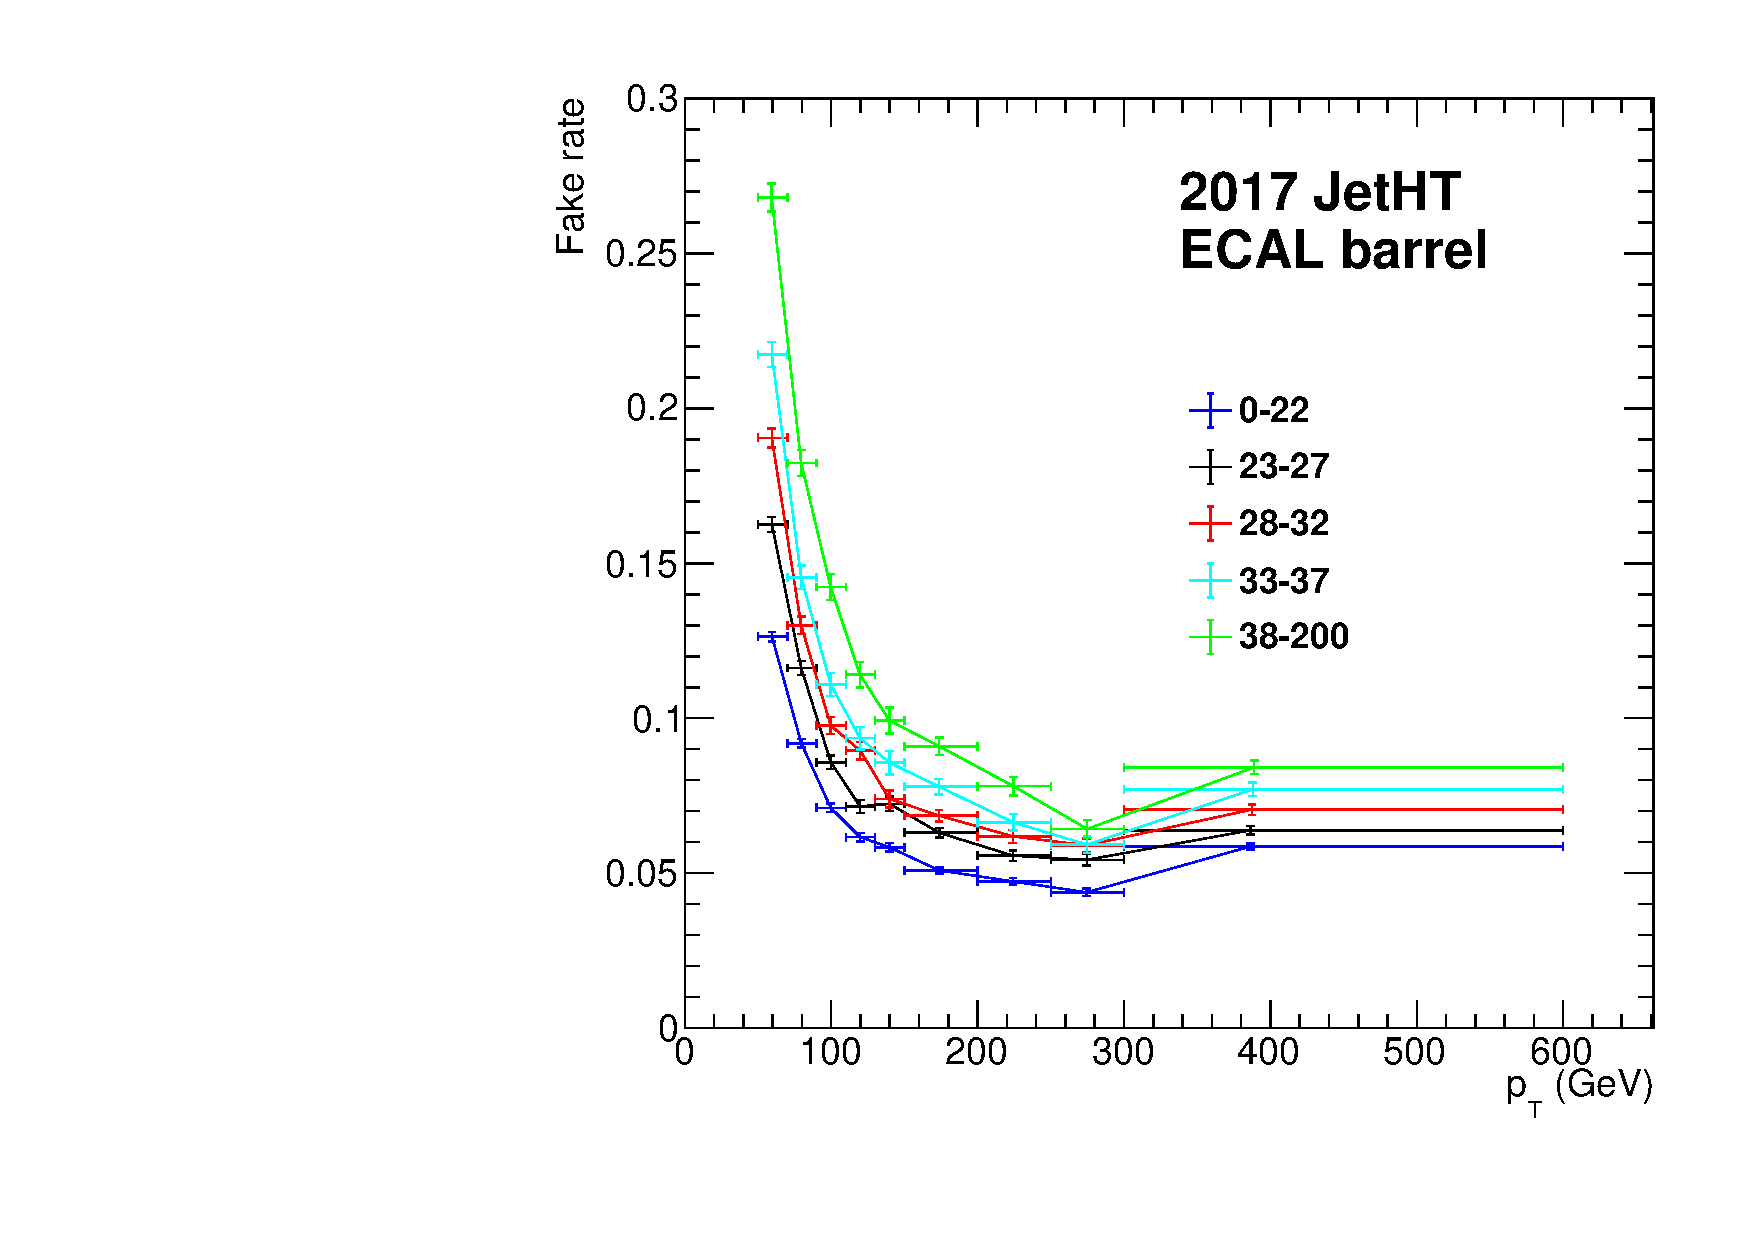
\includegraphics[width=0.3\textwidth]{fig/compare_pv_EB_2017_jetht.pdf}
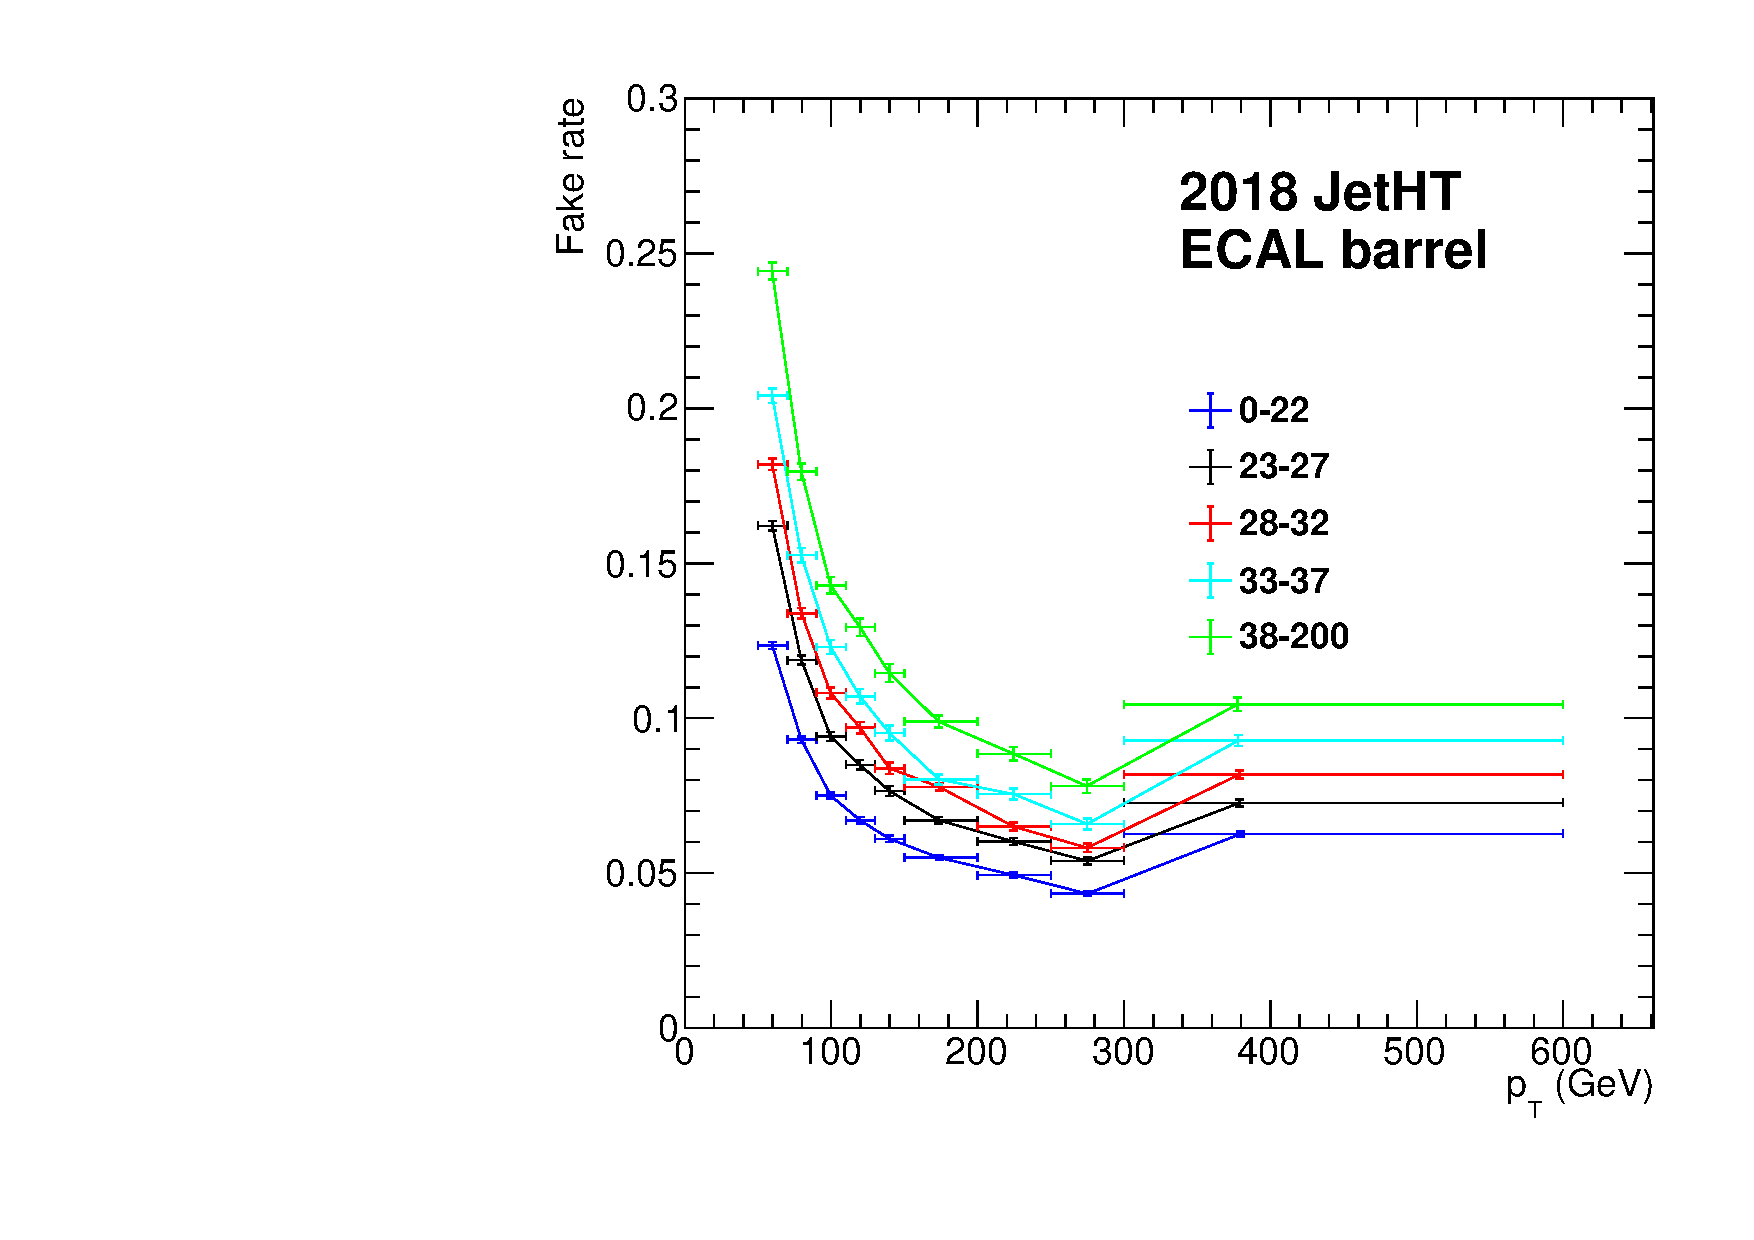
\includegraphics[width=0.3\textwidth]{fig/compare_pv_EB_2018_jetht.pdf}\\
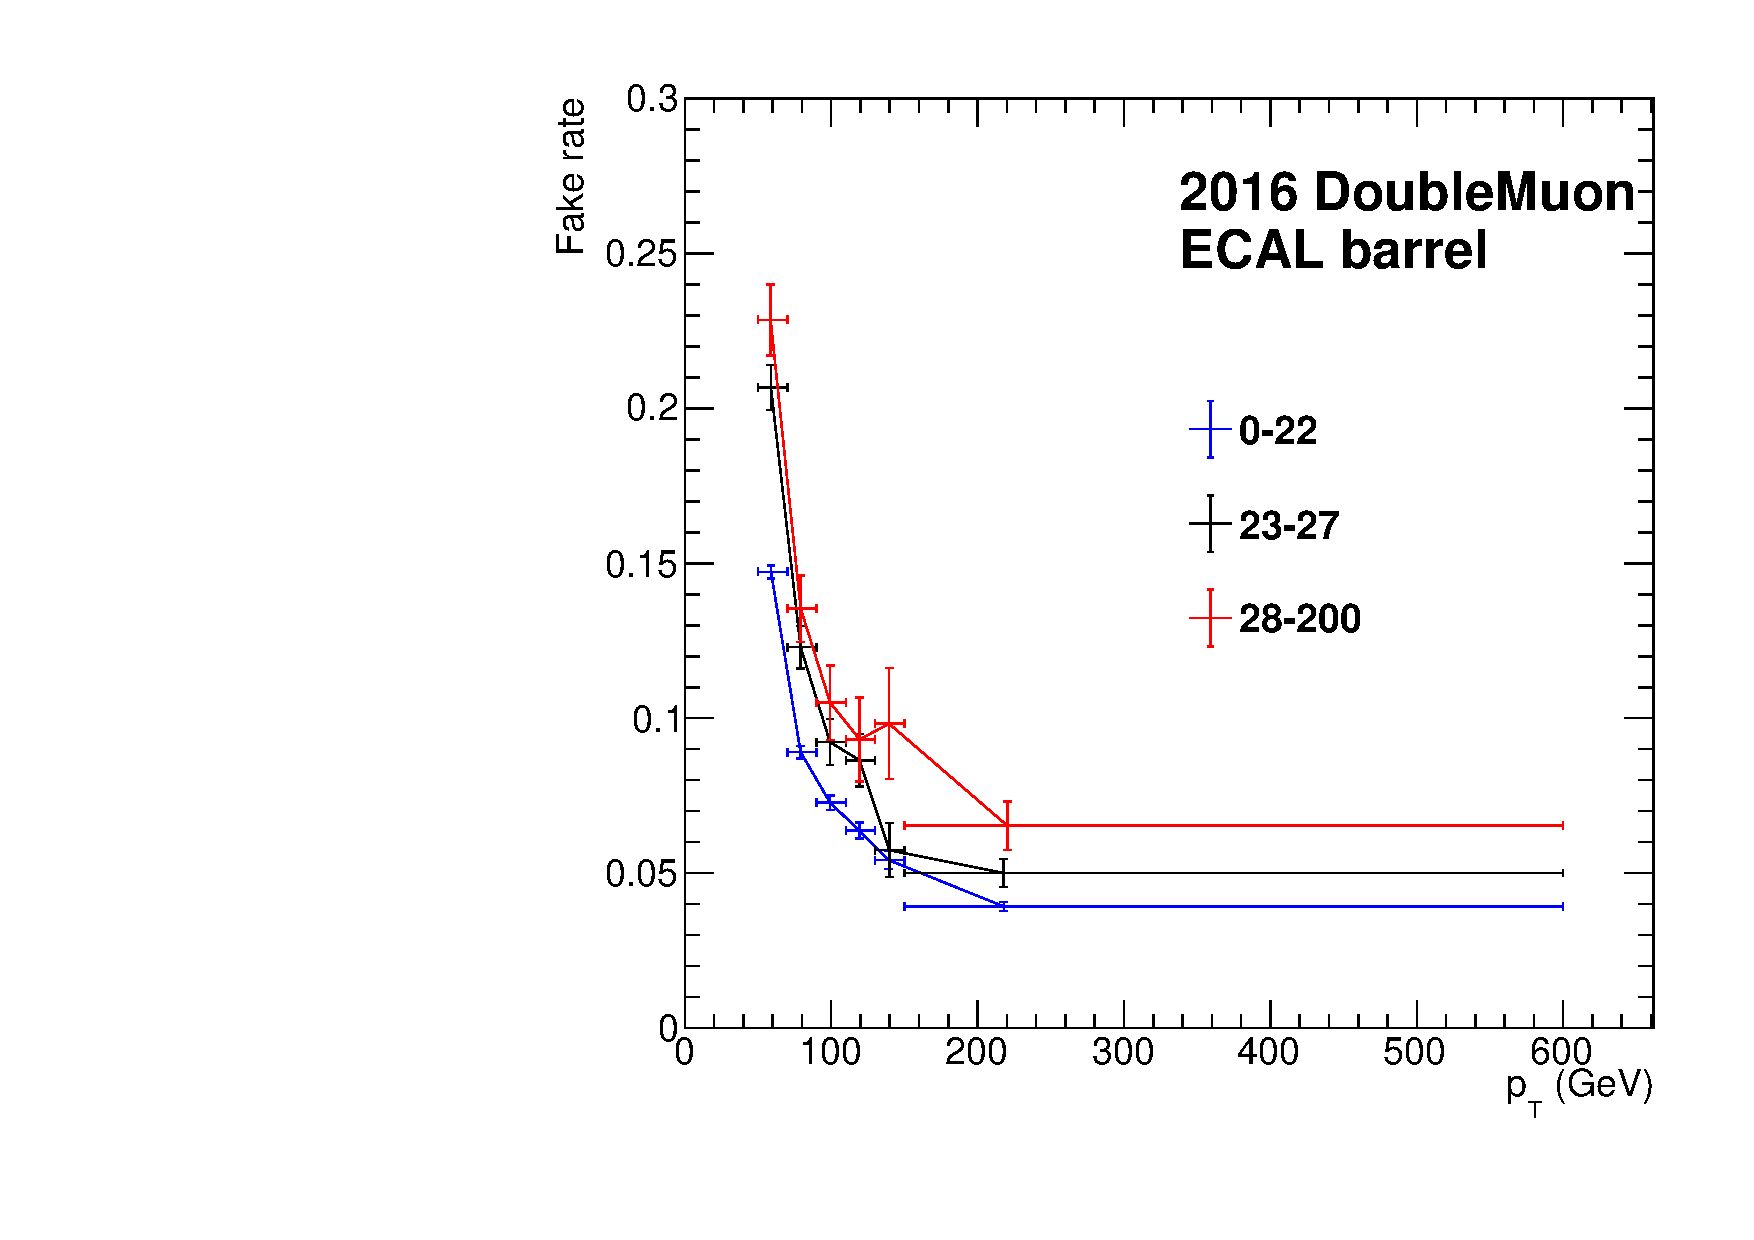
\includegraphics[width=0.3\textwidth]{fig/compare_pv_EB_2016_doublemuon.pdf}
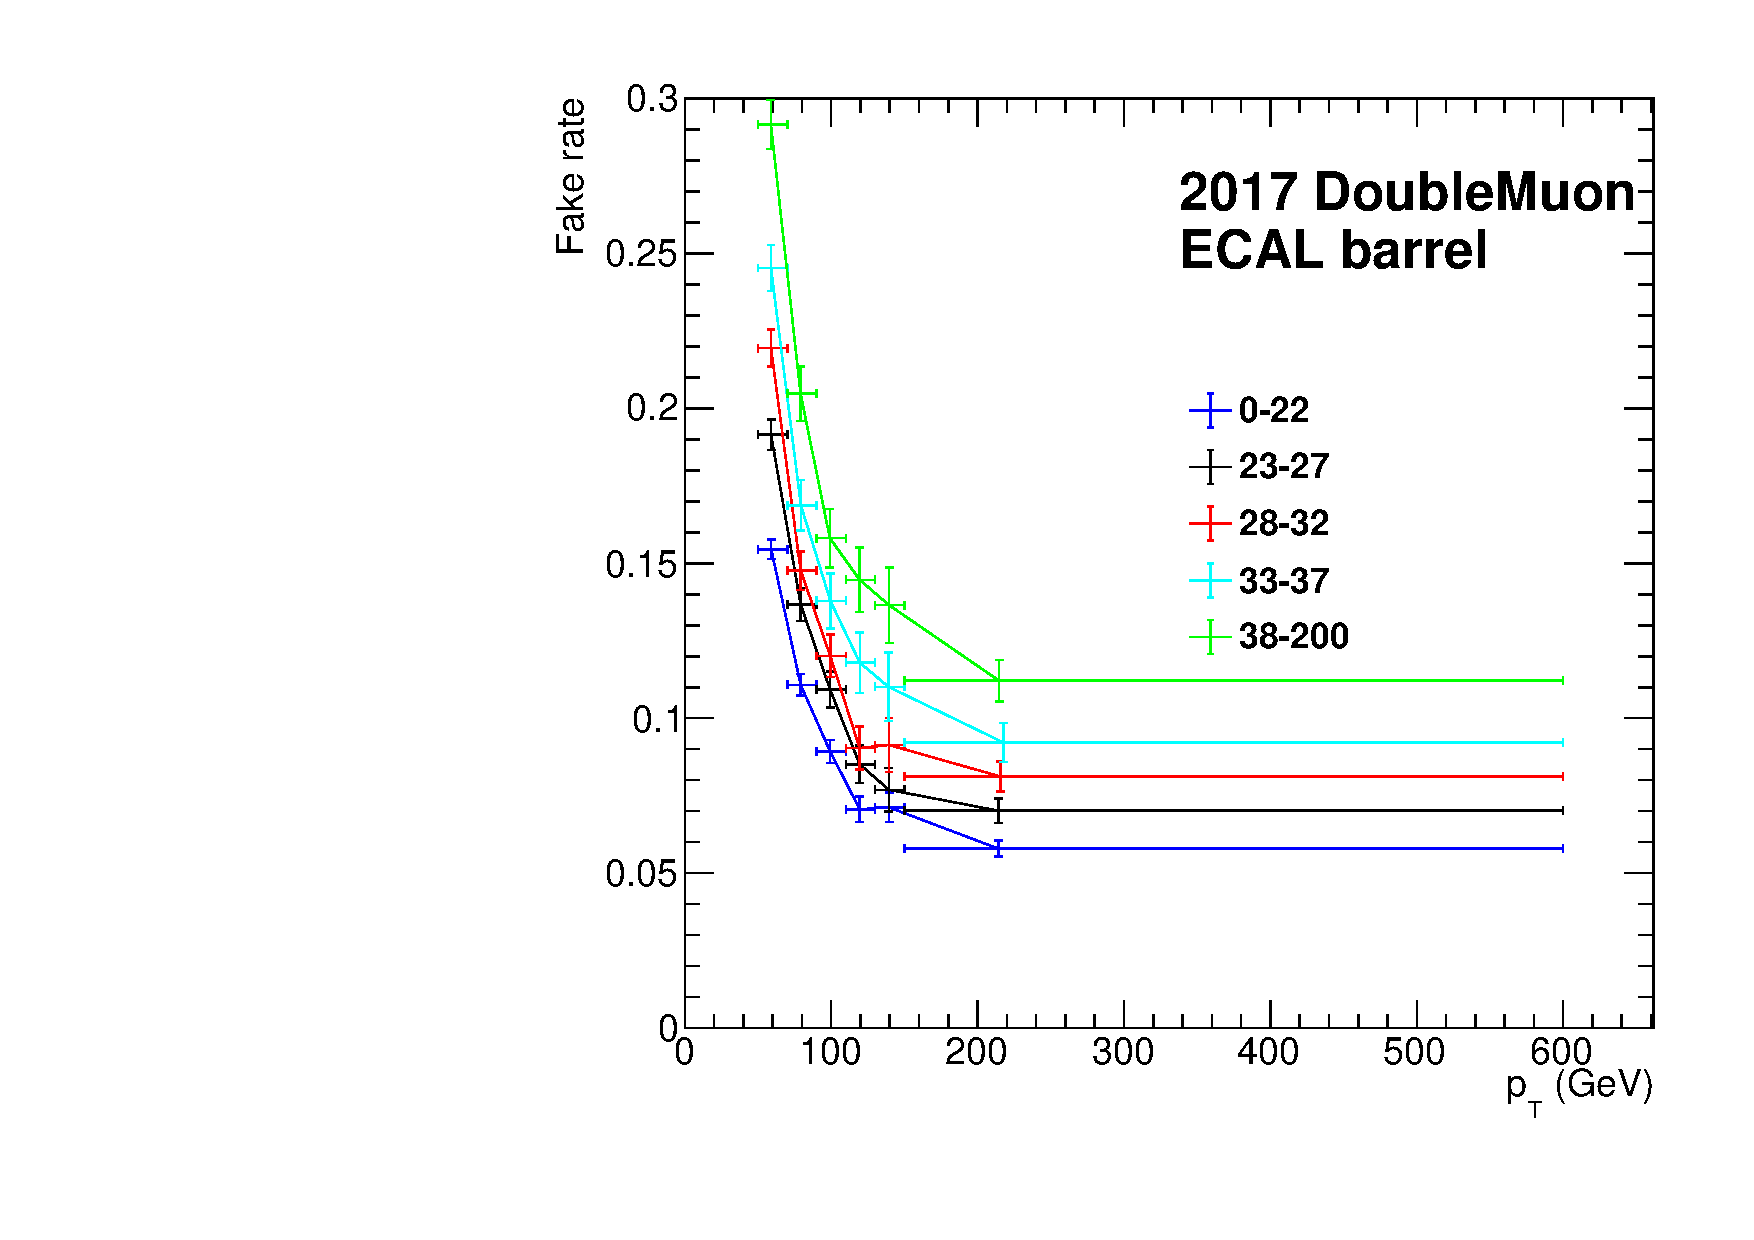
\includegraphics[width=0.3\textwidth]{fig/compare_pv_EB_2017_doublemuon.pdf}
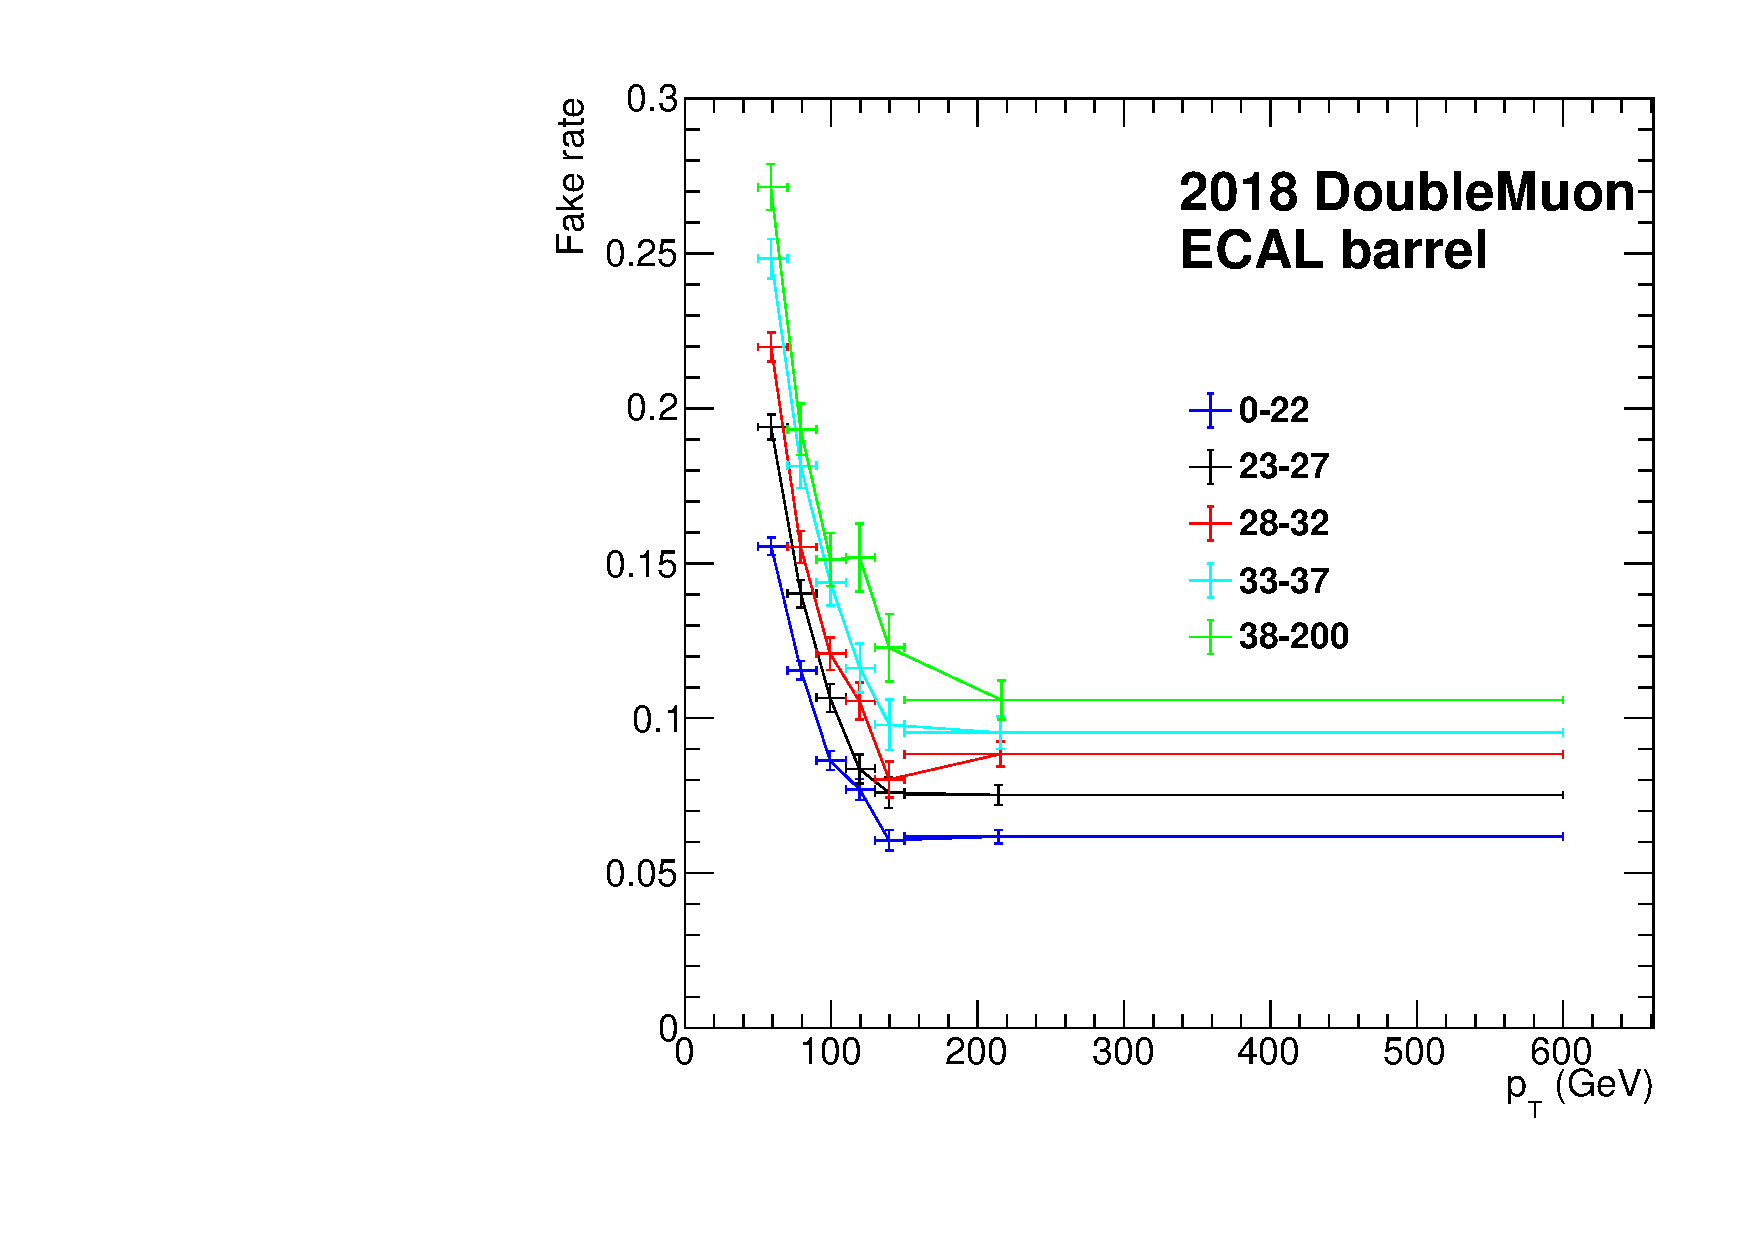
\includegraphics[width=0.3\textwidth]{fig/compare_pv_EB_2018_doublemuon.pdf}
\label{fig:frpileup_EB}
\end{figure}

% % generated by compare_pv.exe
\begin{figure}[!htbp]
\caption{A comparison of the fake rate in EE1 ($1.566 < |\eta| < 2.033$) measured as a function of the number of selected primary vertices in the event using the \texttt{JetHT} data set (top) and \texttt{DoubleMuon} data set (bottom). The fake rates are determined separately for 2016 (left), 2017 (center), and 2018 (right).}
\centering
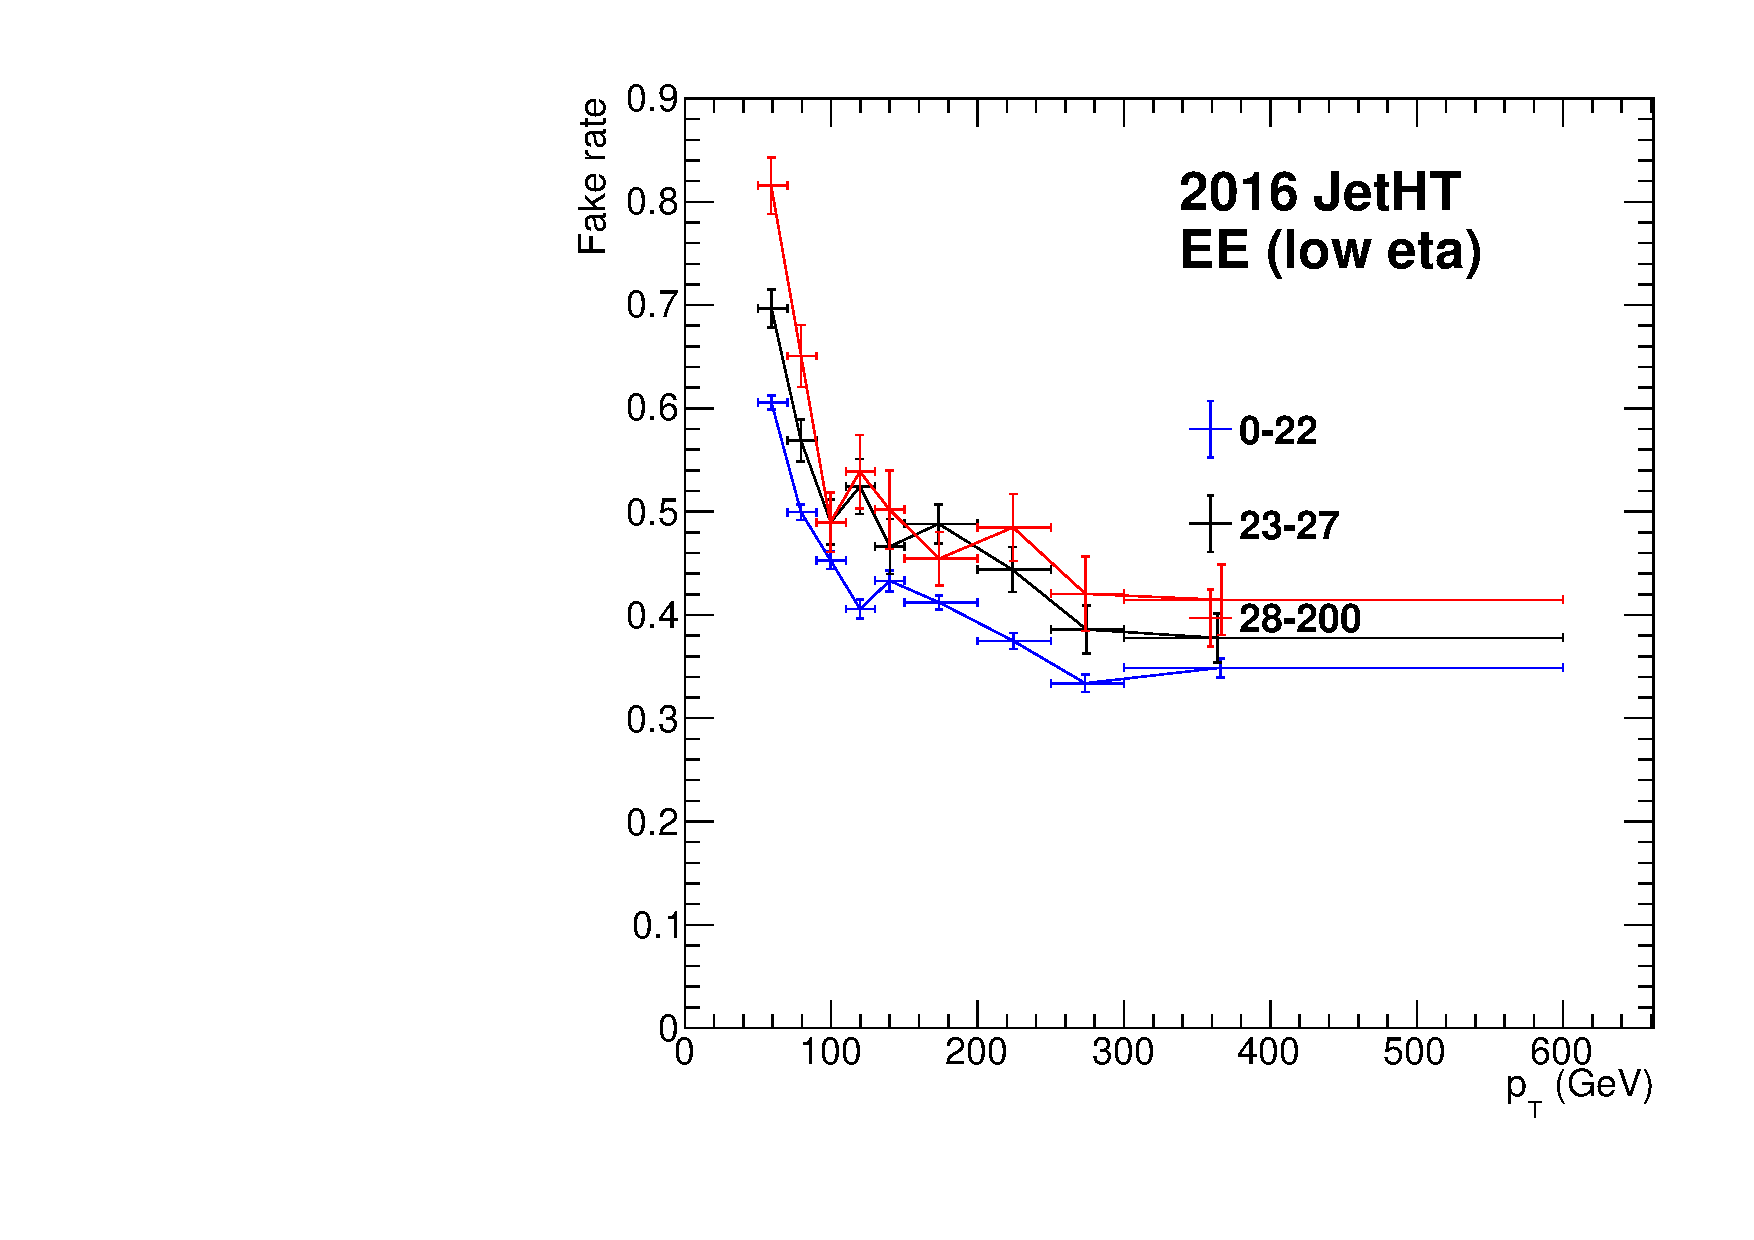
\includegraphics[width=0.3\textwidth]{fig/compare_pv_EE1_2016_jetht.pdf}
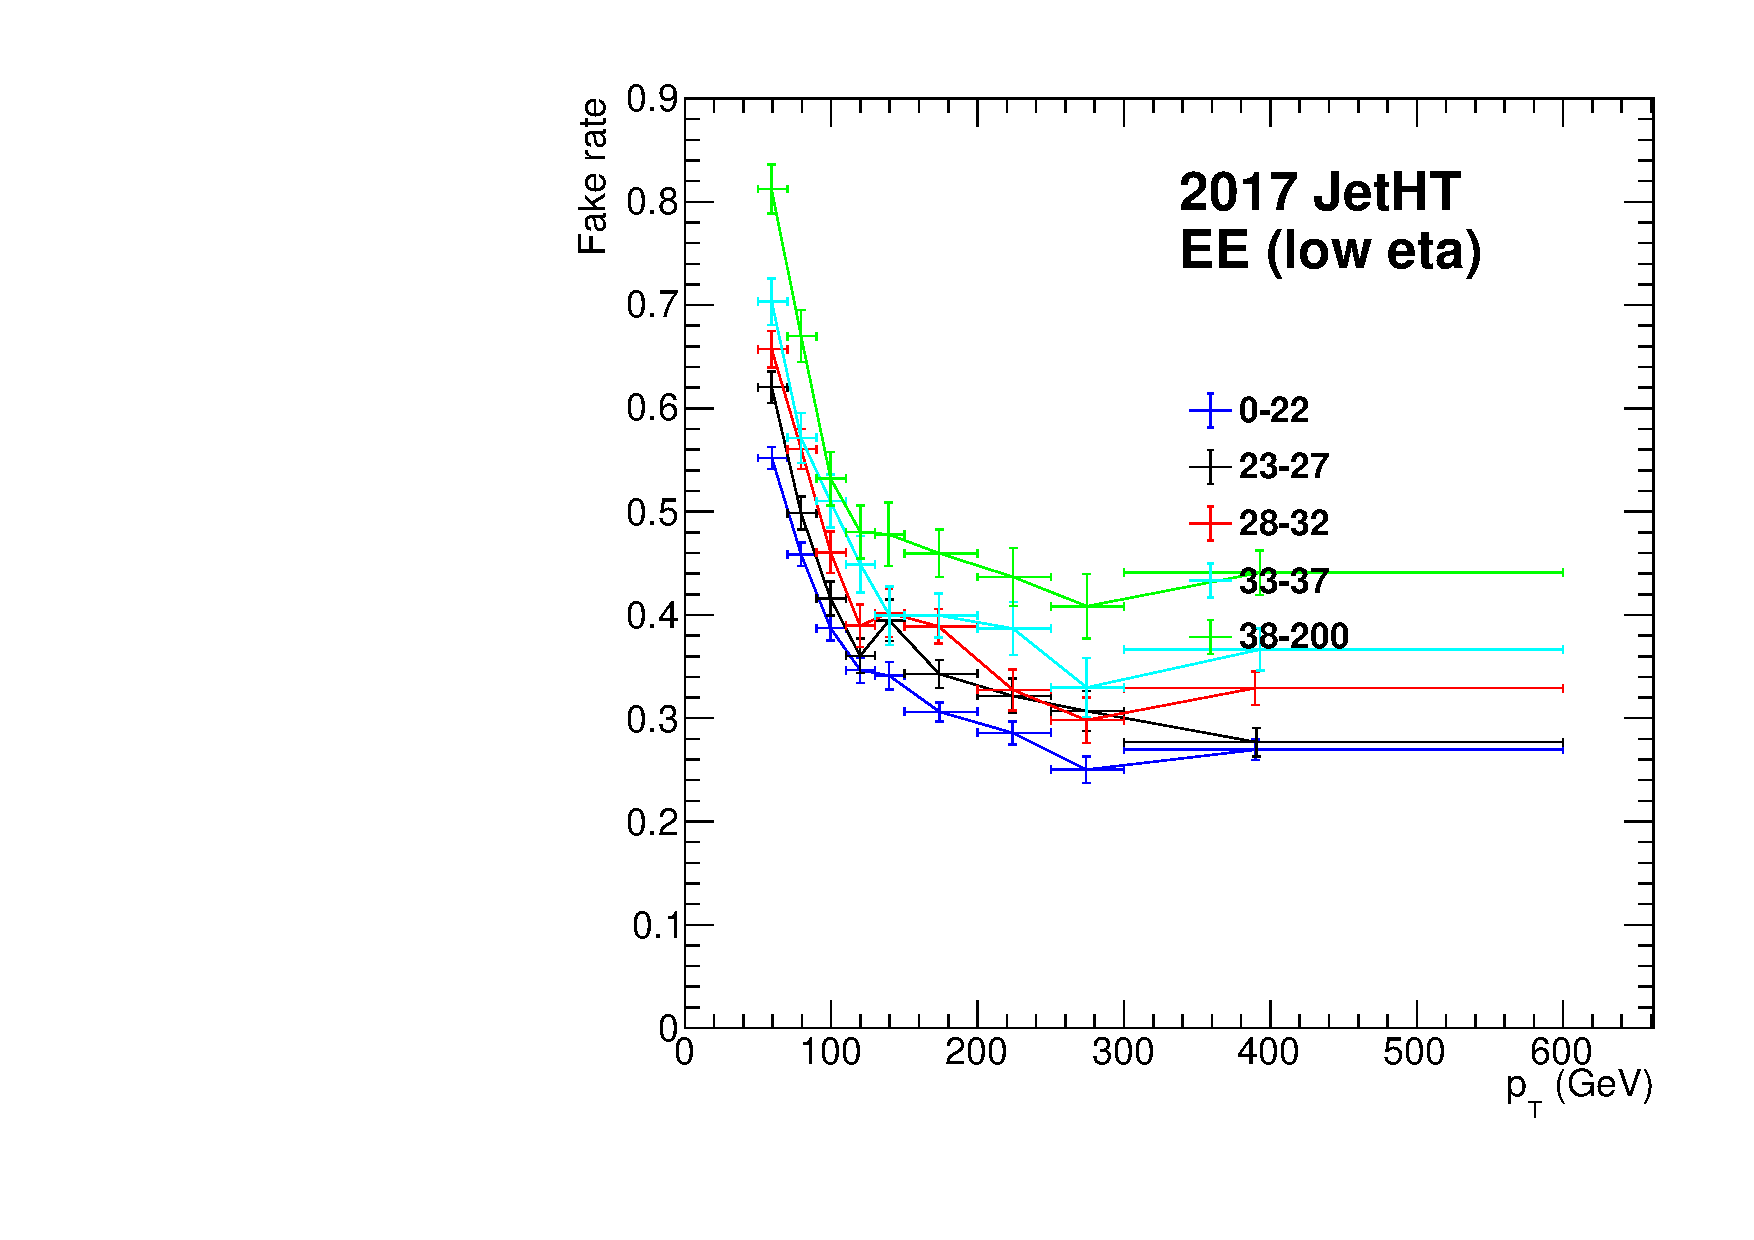
\includegraphics[width=0.3\textwidth]{fig/compare_pv_EE1_2017_jetht.pdf}
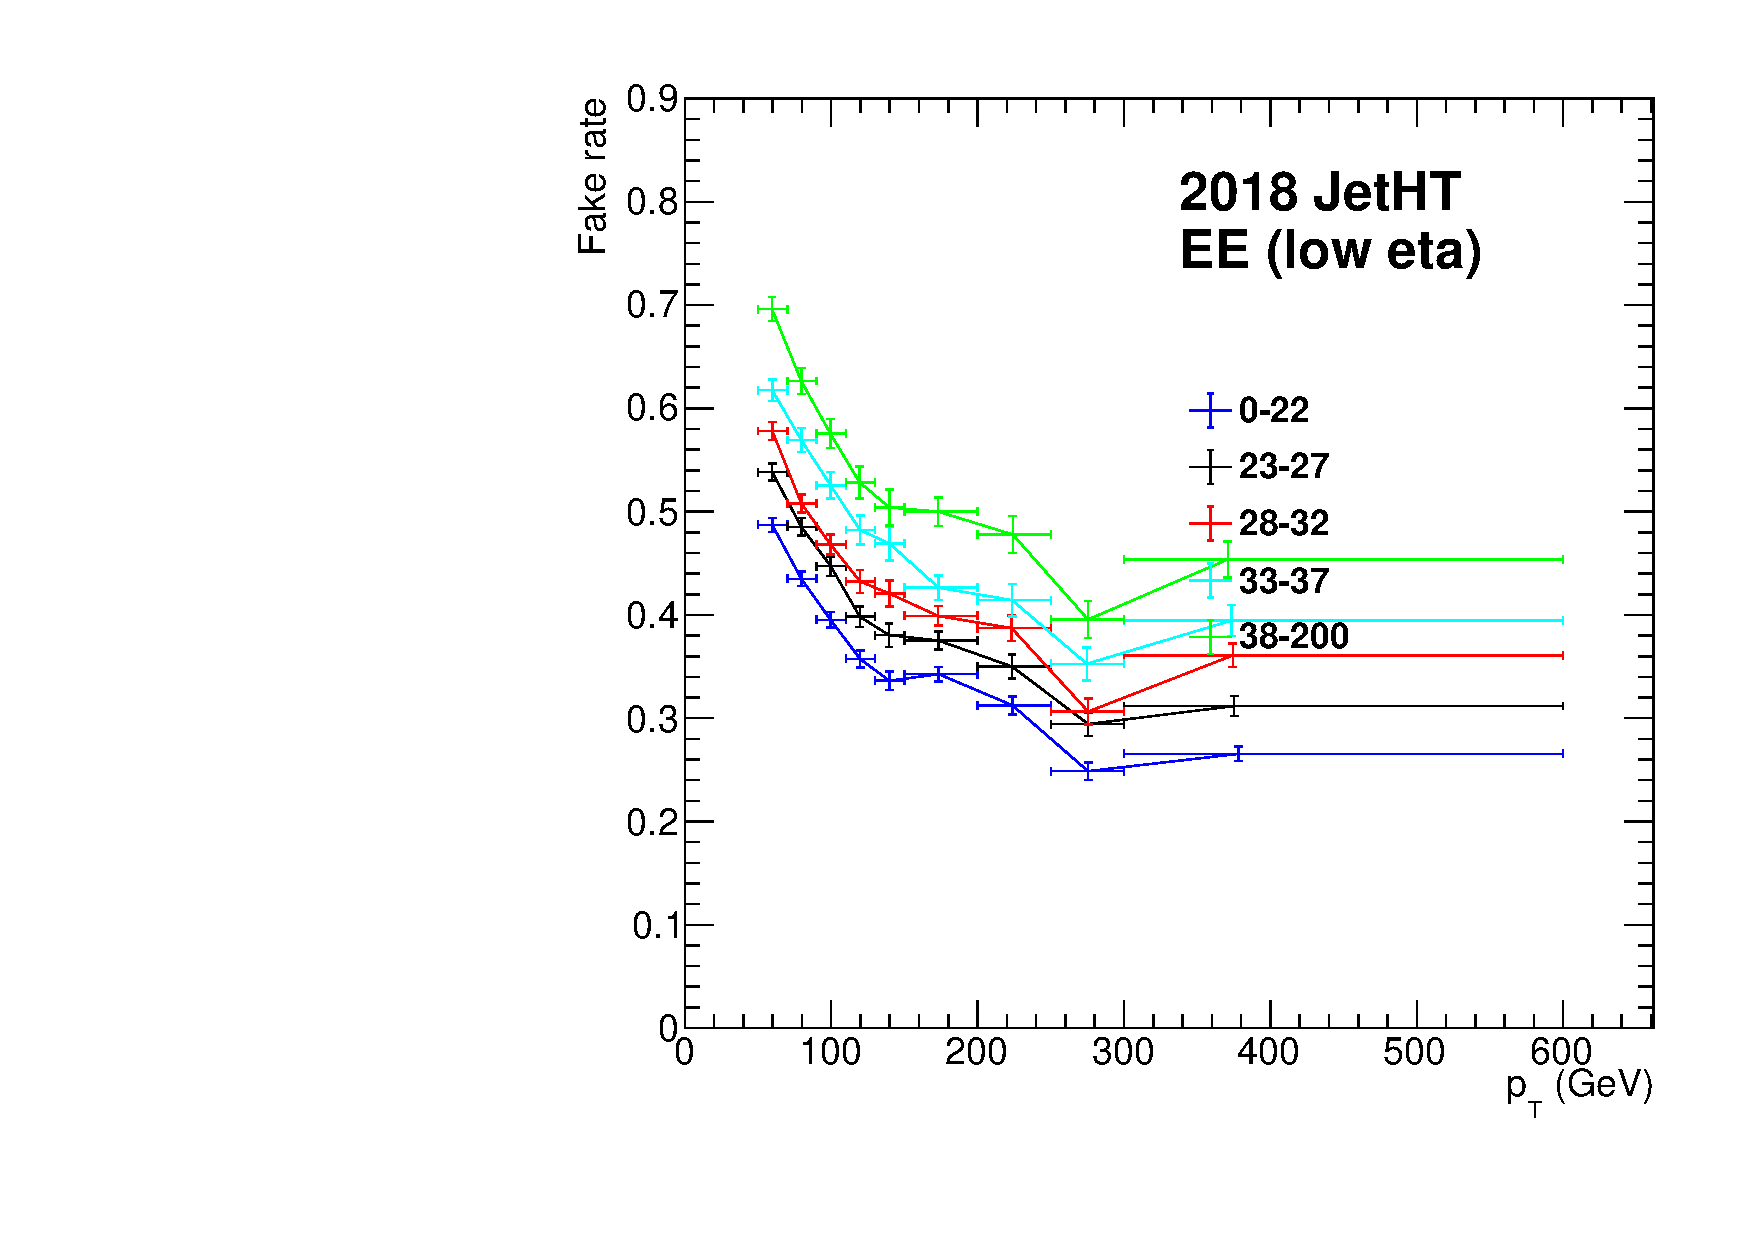
\includegraphics[width=0.3\textwidth]{fig/compare_pv_EE1_2018_jetht.pdf}
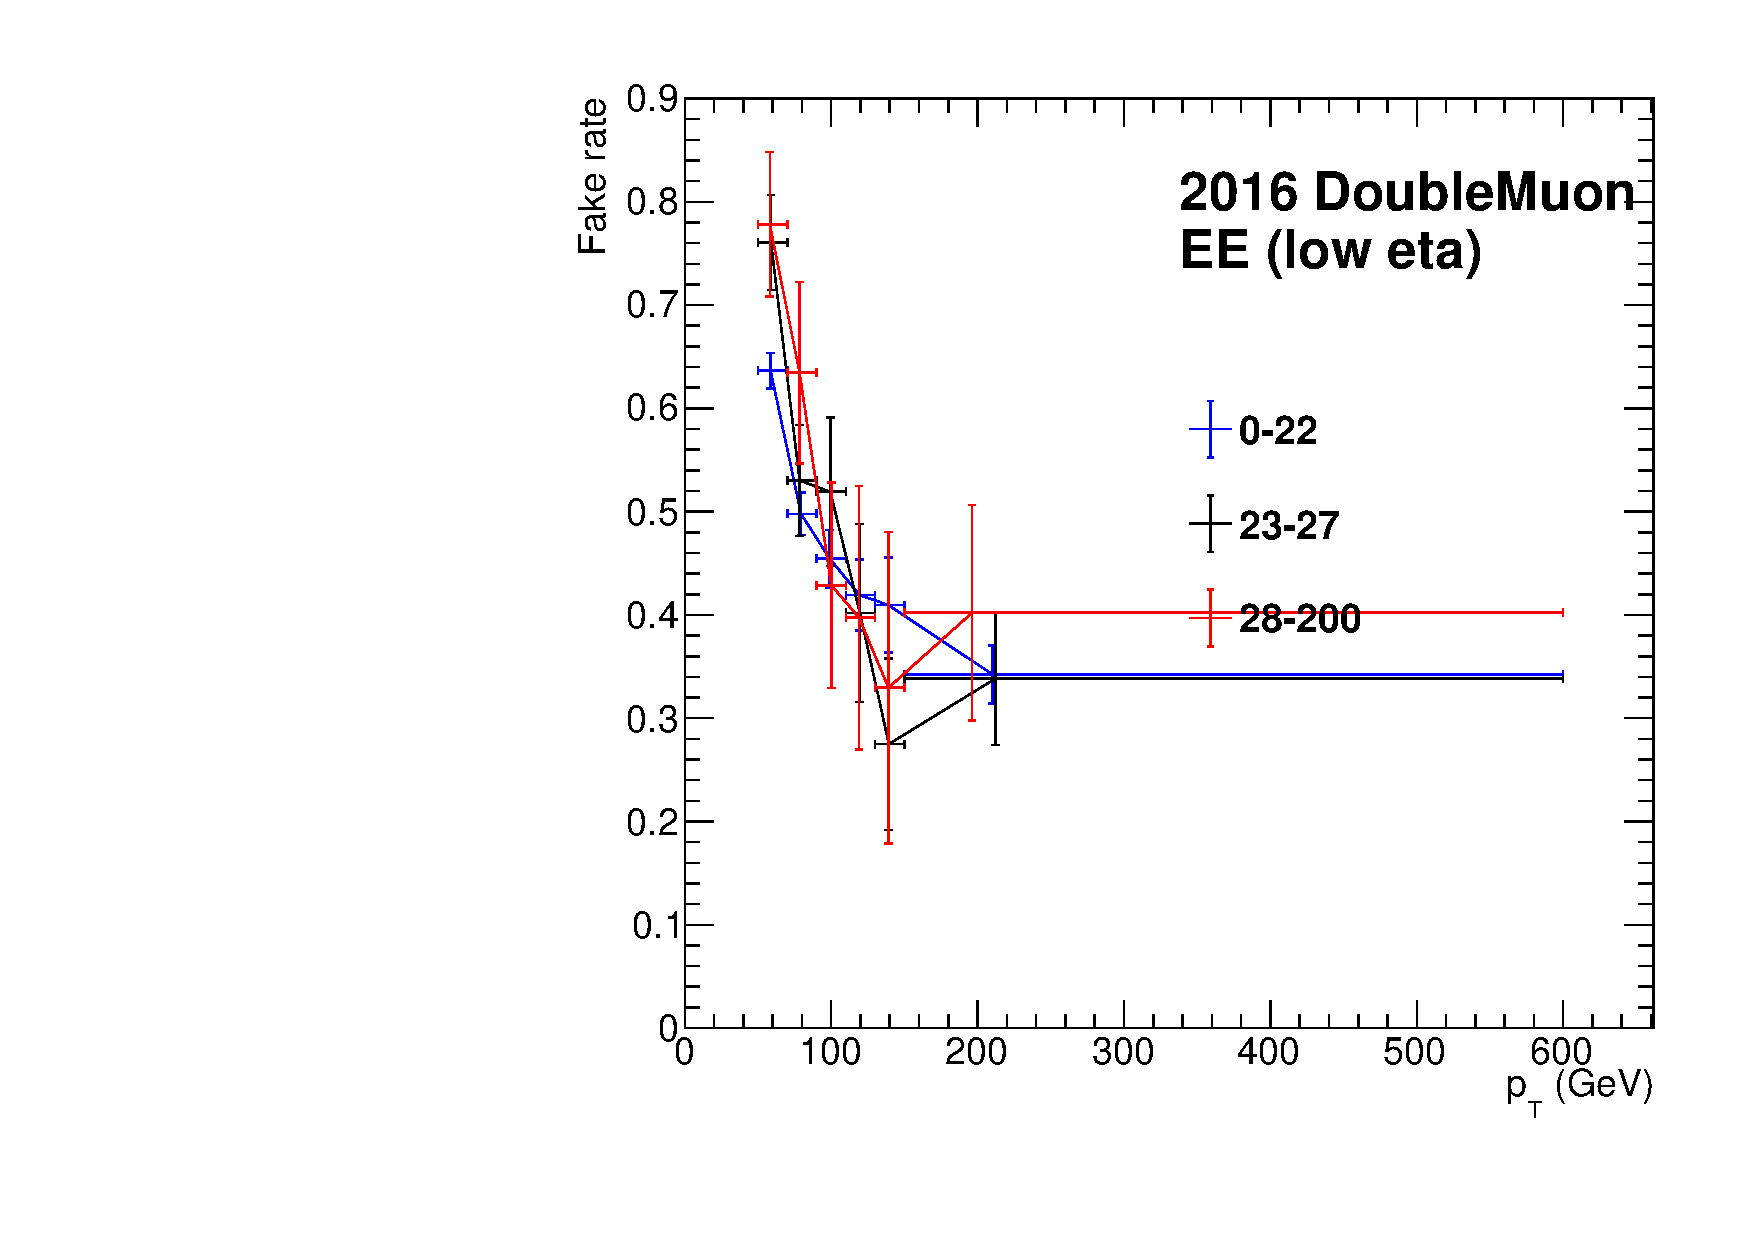
\includegraphics[width=0.3\textwidth]{fig/compare_pv_EE1_2016_doublemuon.pdf}
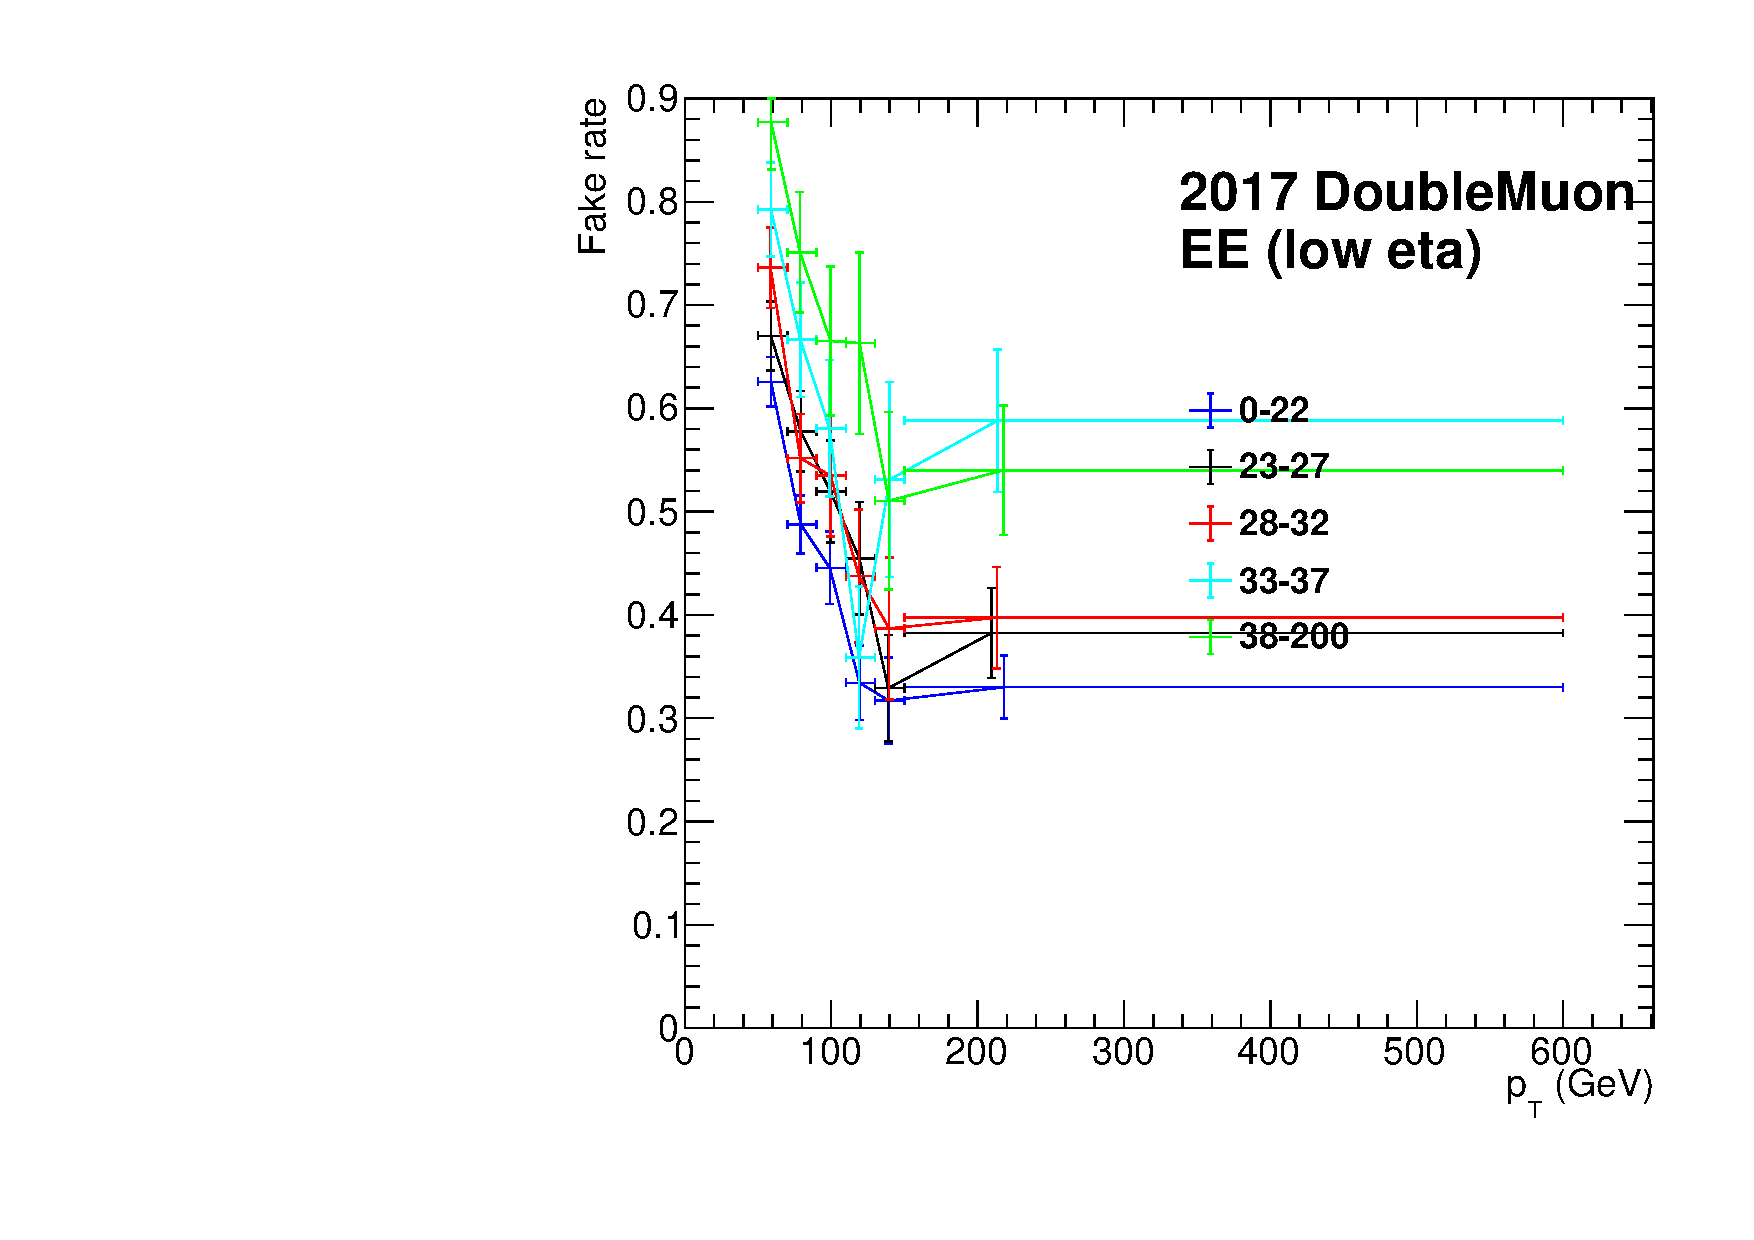
\includegraphics[width=0.3\textwidth]{fig/compare_pv_EE1_2017_doublemuon.pdf}
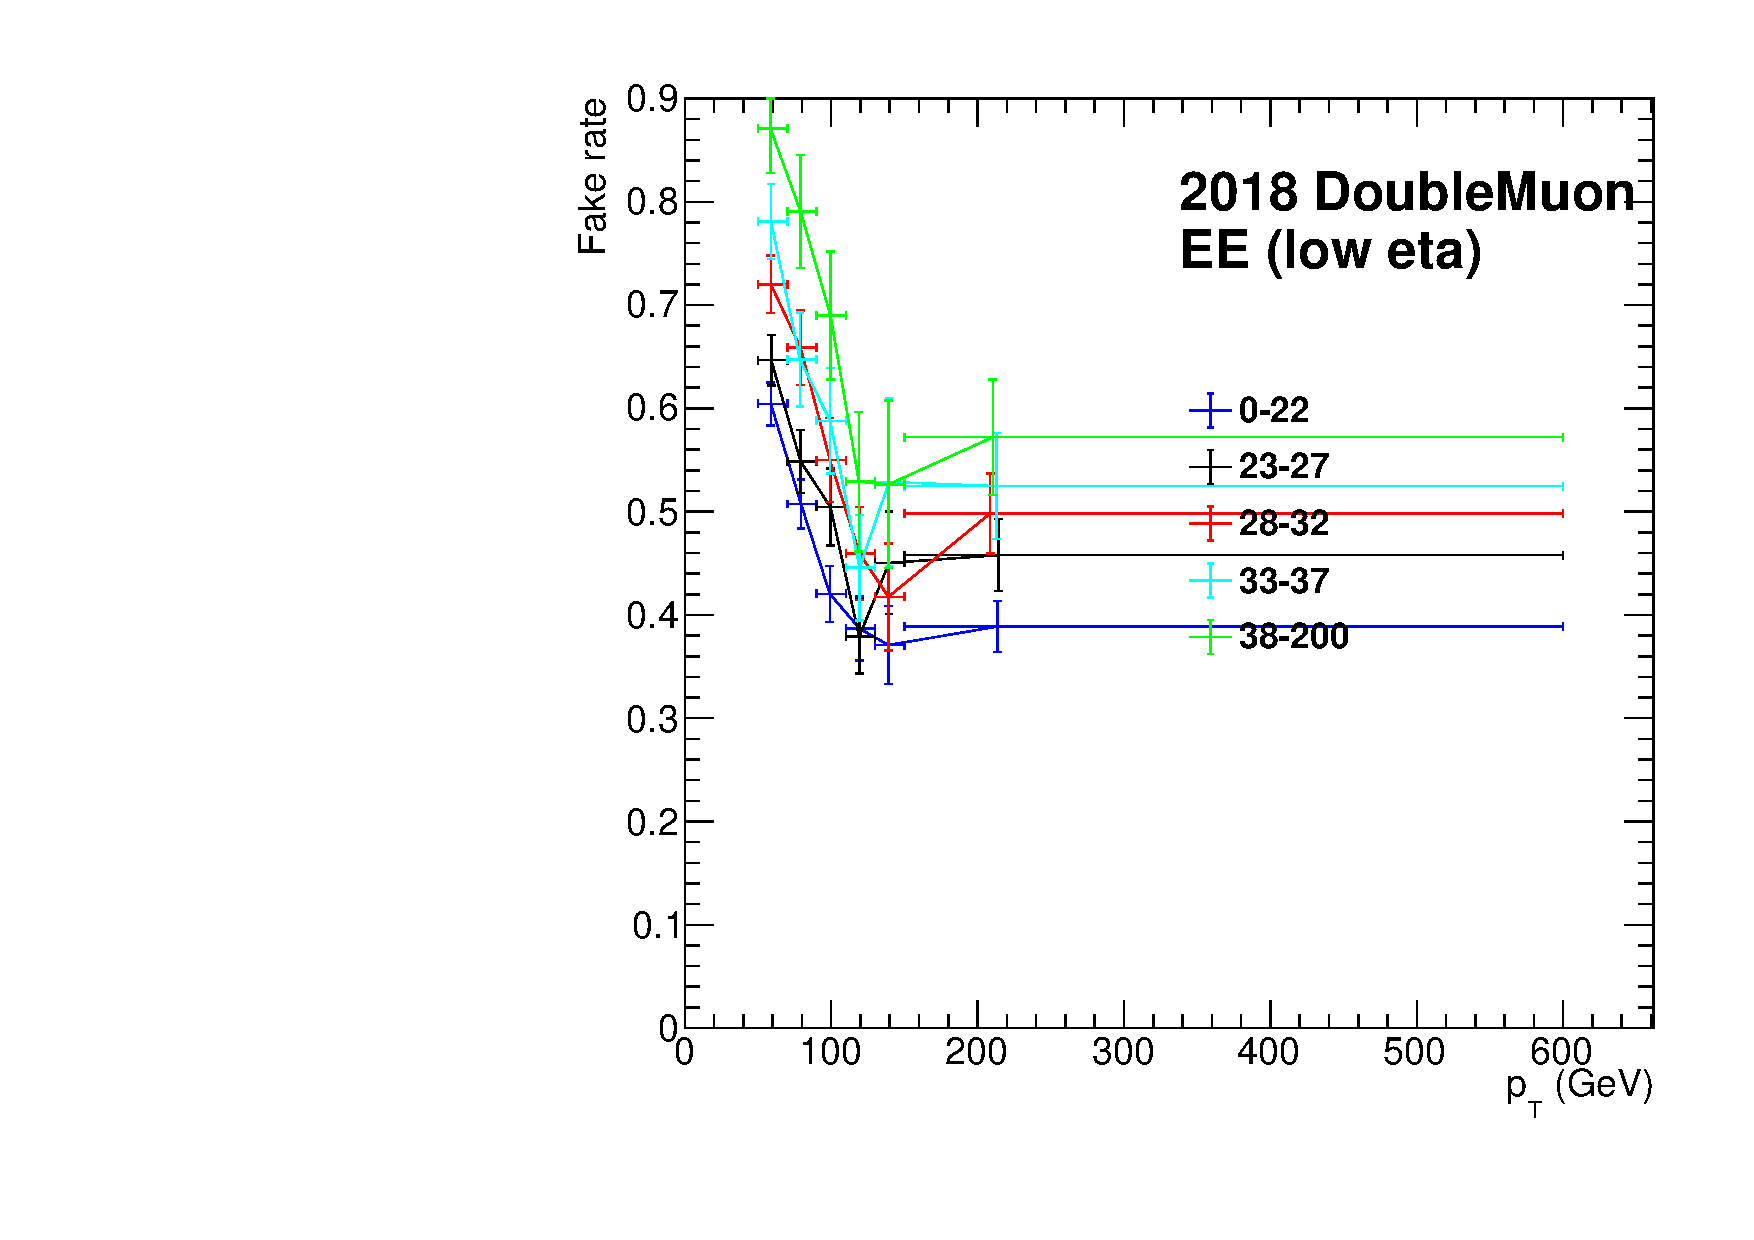
\includegraphics[width=0.3\textwidth]{fig/compare_pv_EE1_2018_doublemuon.pdf}
\label{fig:frpileup_EE1}
\end{figure}


% generated by compare_pv.exe
\begin{figure}[!htbp]
\caption{A comparison of the fake rate in EE2 ($2.033 \mathopen< \lvert \eta \rvert \mathclose< 2.5$) measured as a function of the number of selected primary vertices in the event using the \texttt{JetHT} data set (top) and \texttt{DoubleMuon} data set (bottom). The fake rates are determined separately for 2016 (left), 2017 (center), and 2018 (right). The ranges used for comparison were chosen to reflect a roughly uniform level of statistics between all ranges.}
\centering
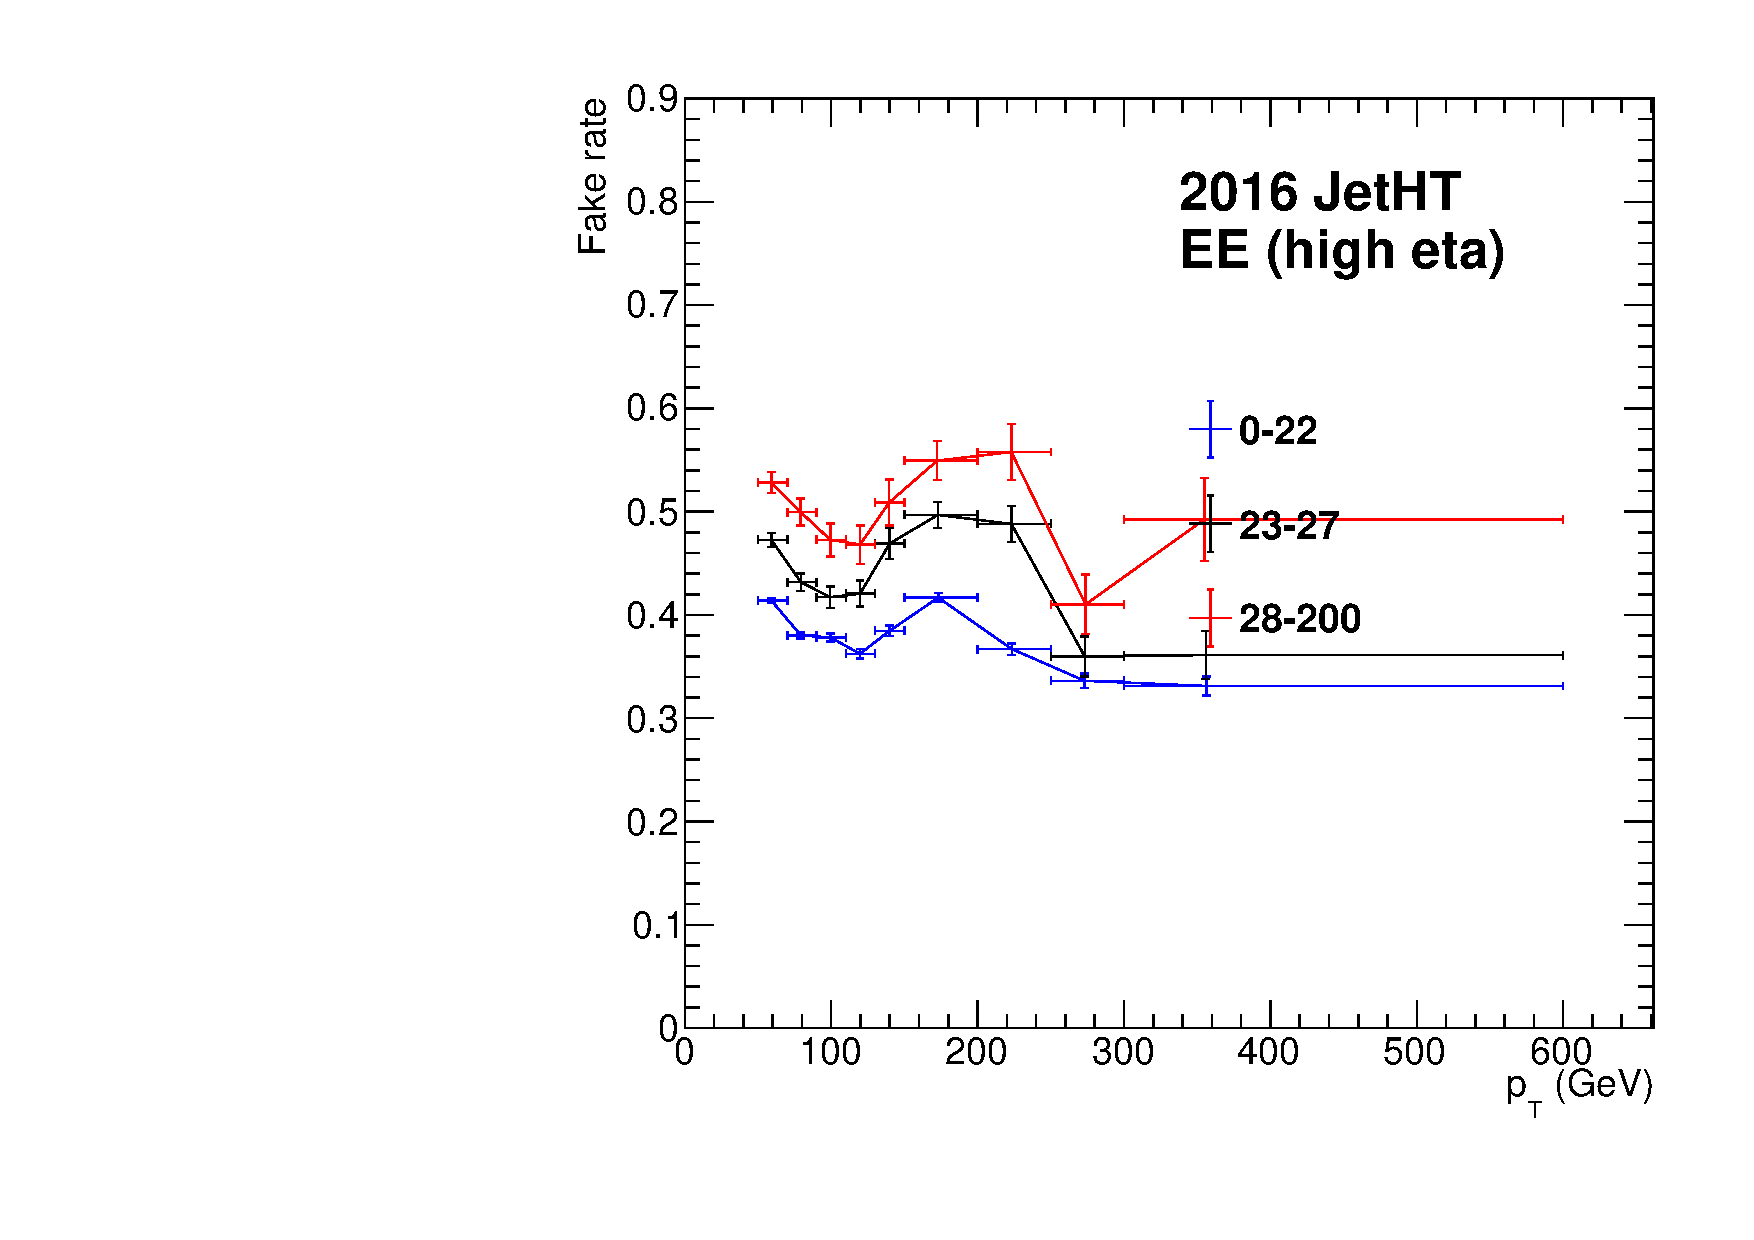
\includegraphics[width=0.3\textwidth]{fig/compare_pv_EE2_2016_jetht.pdf}
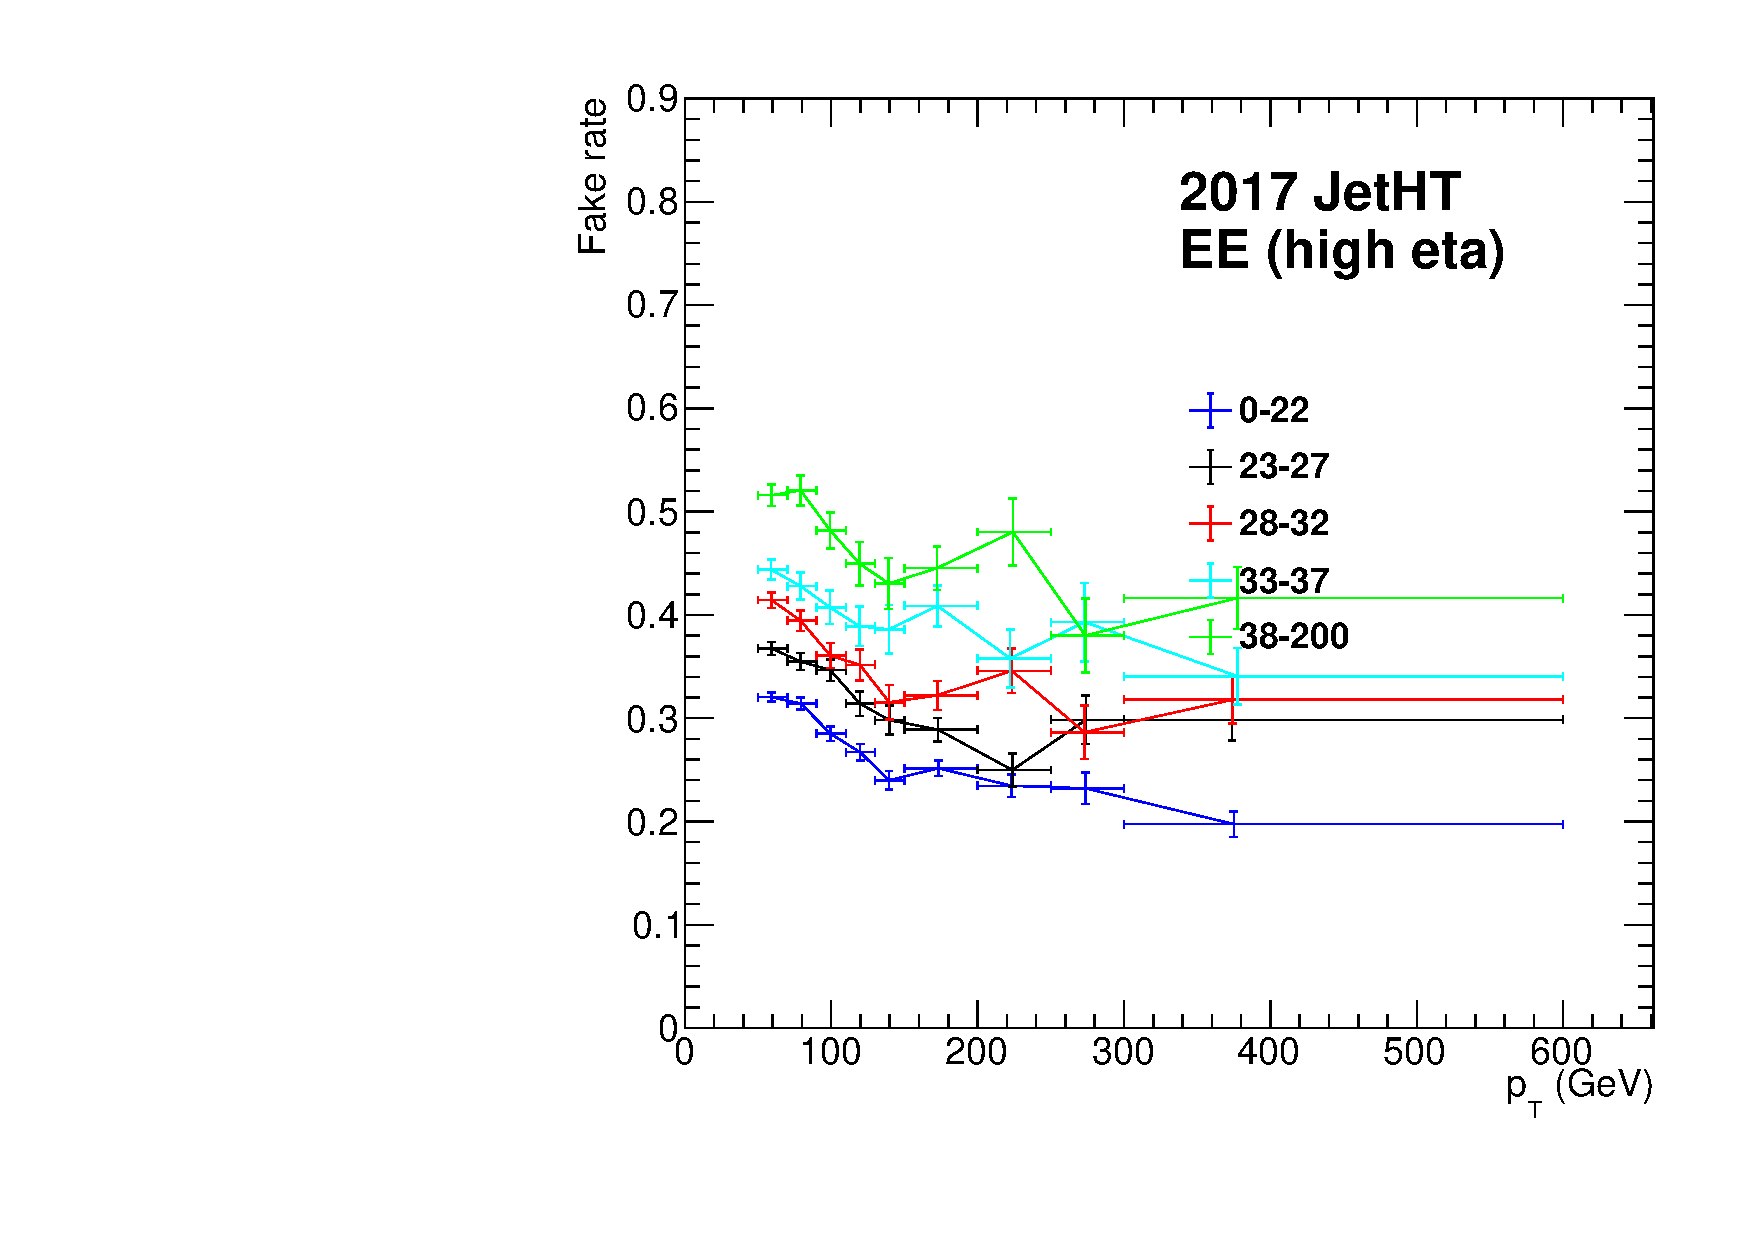
\includegraphics[width=0.3\textwidth]{fig/compare_pv_EE2_2017_jetht.pdf}
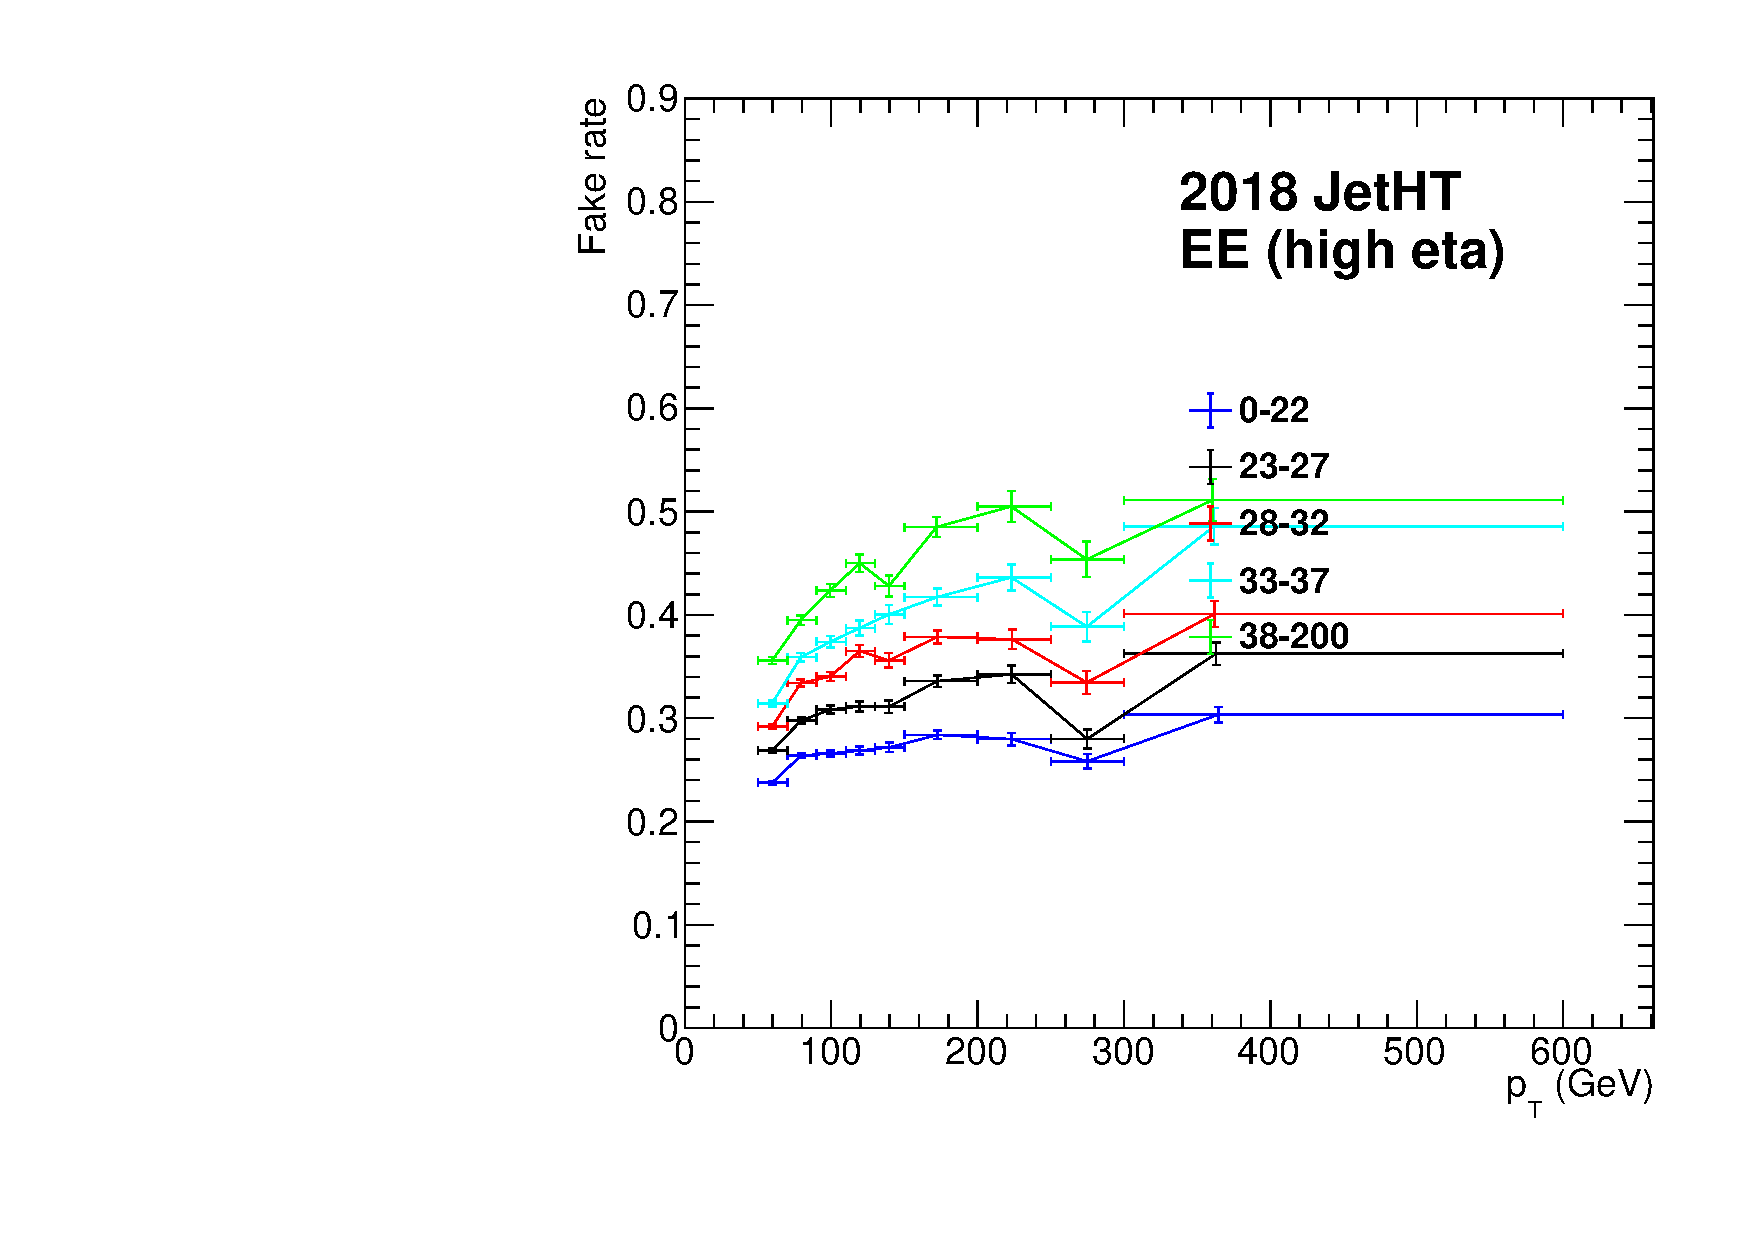
\includegraphics[width=0.3\textwidth]{fig/compare_pv_EE2_2018_jetht.pdf}
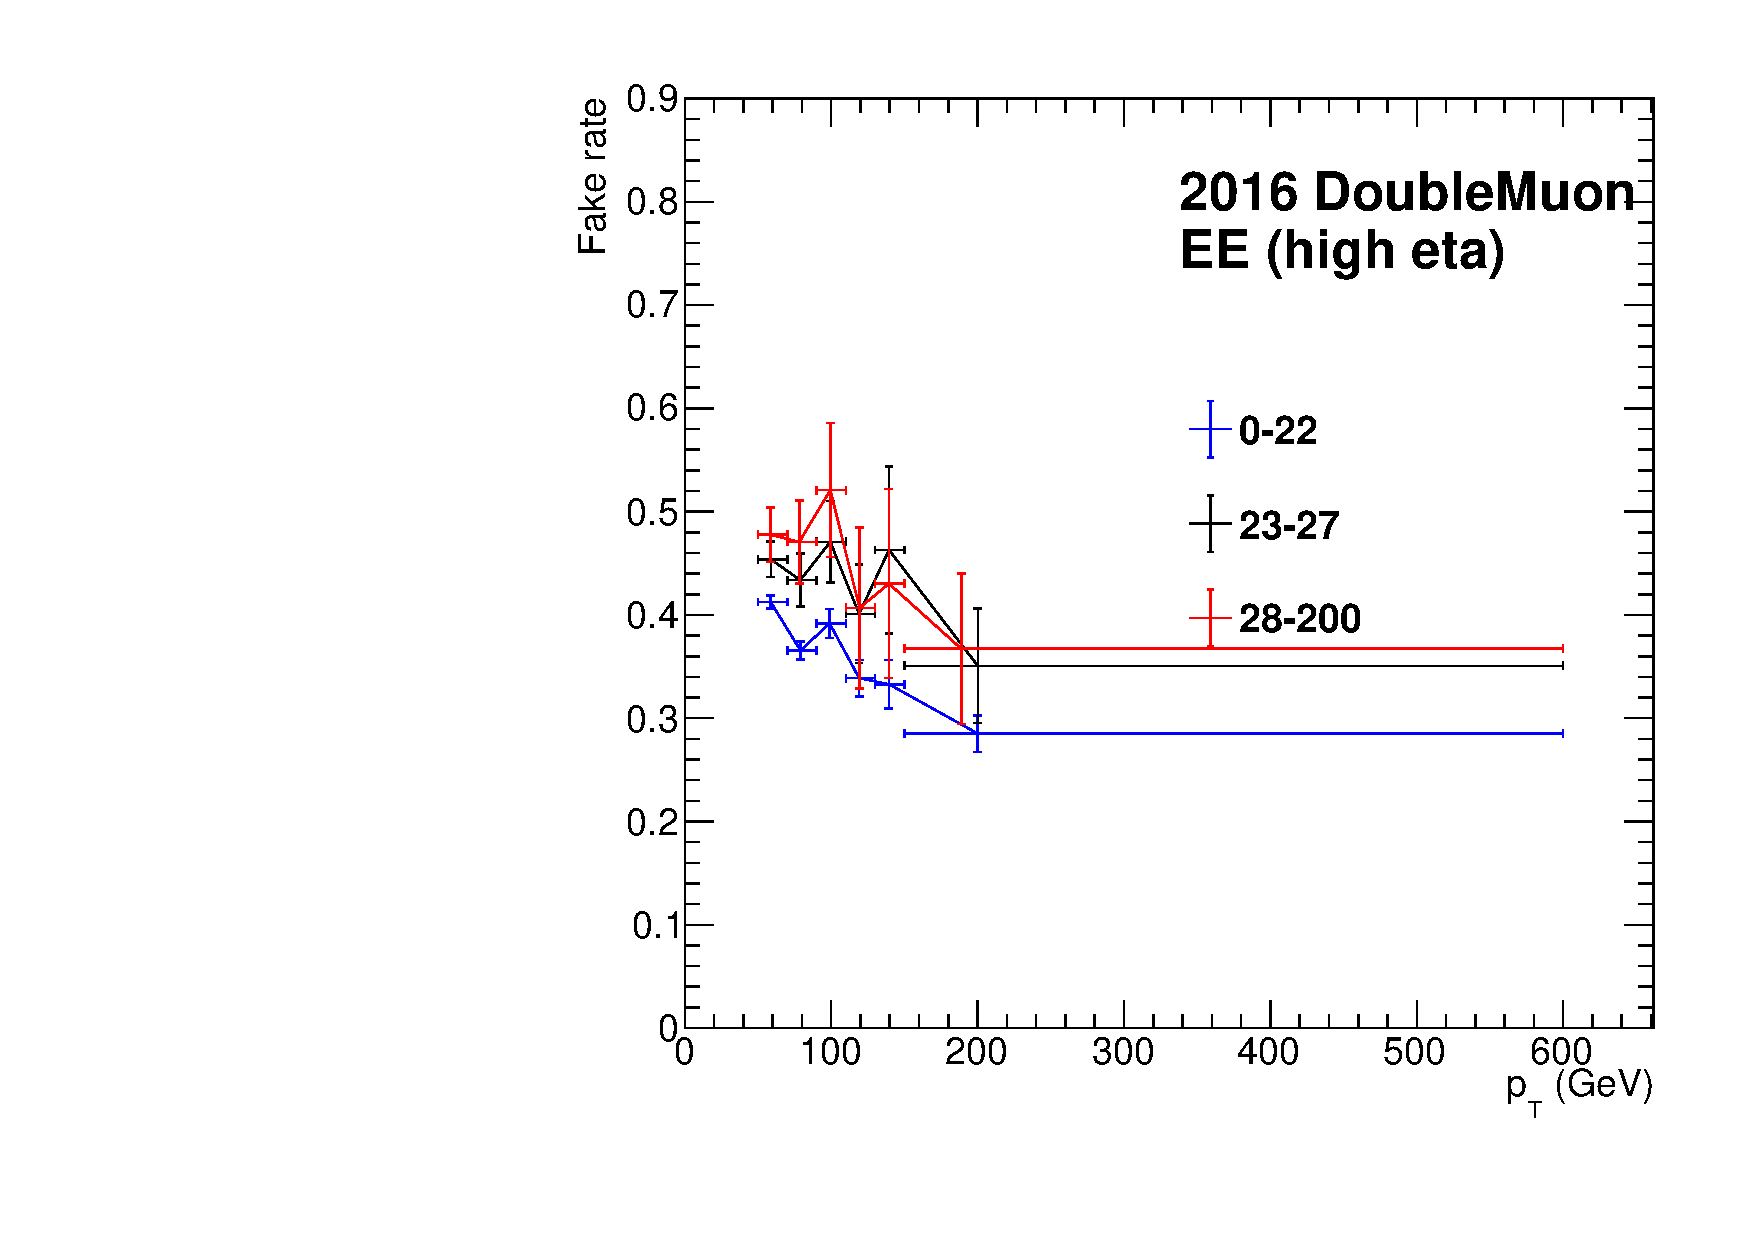
\includegraphics[width=0.3\textwidth]{fig/compare_pv_EE2_2016_doublemuon.pdf}
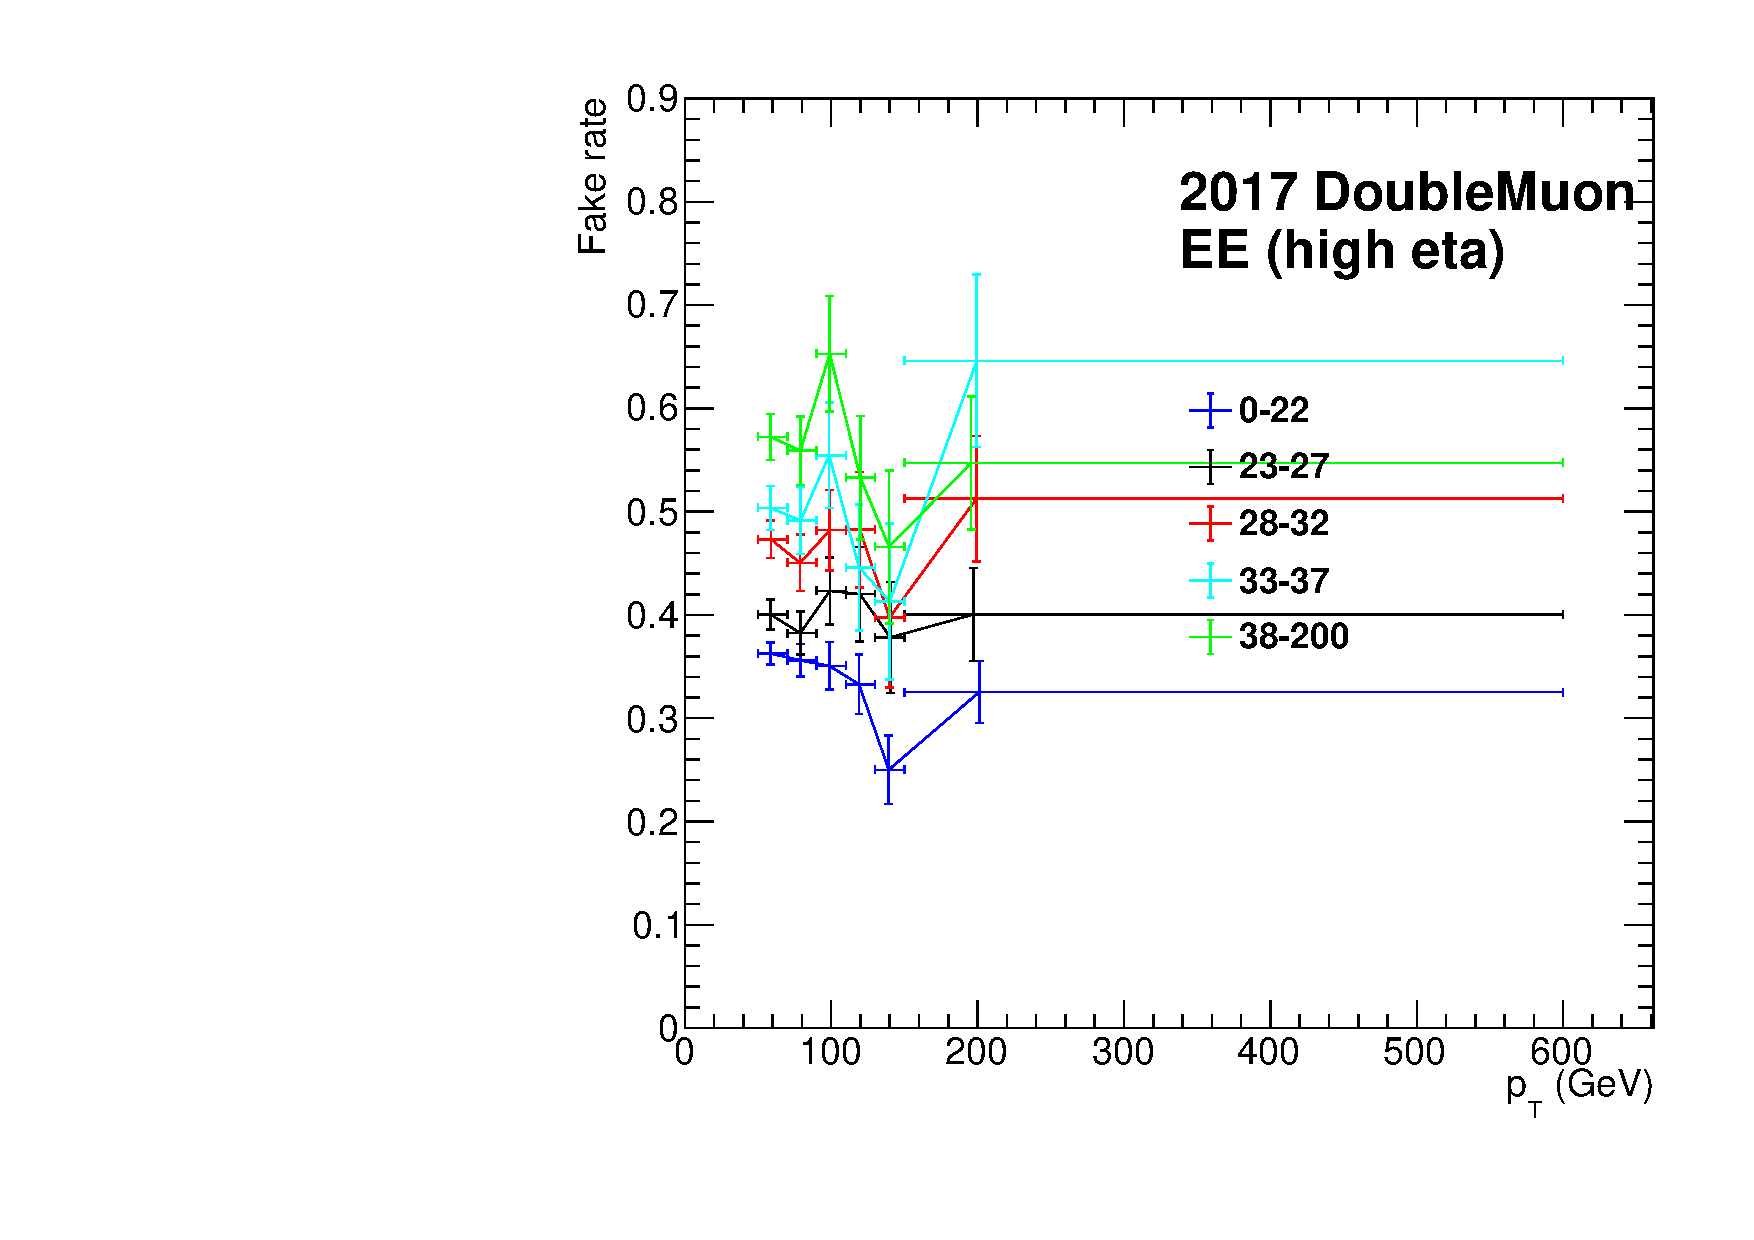
\includegraphics[width=0.3\textwidth]{fig/compare_pv_EE2_2017_doublemuon.pdf}
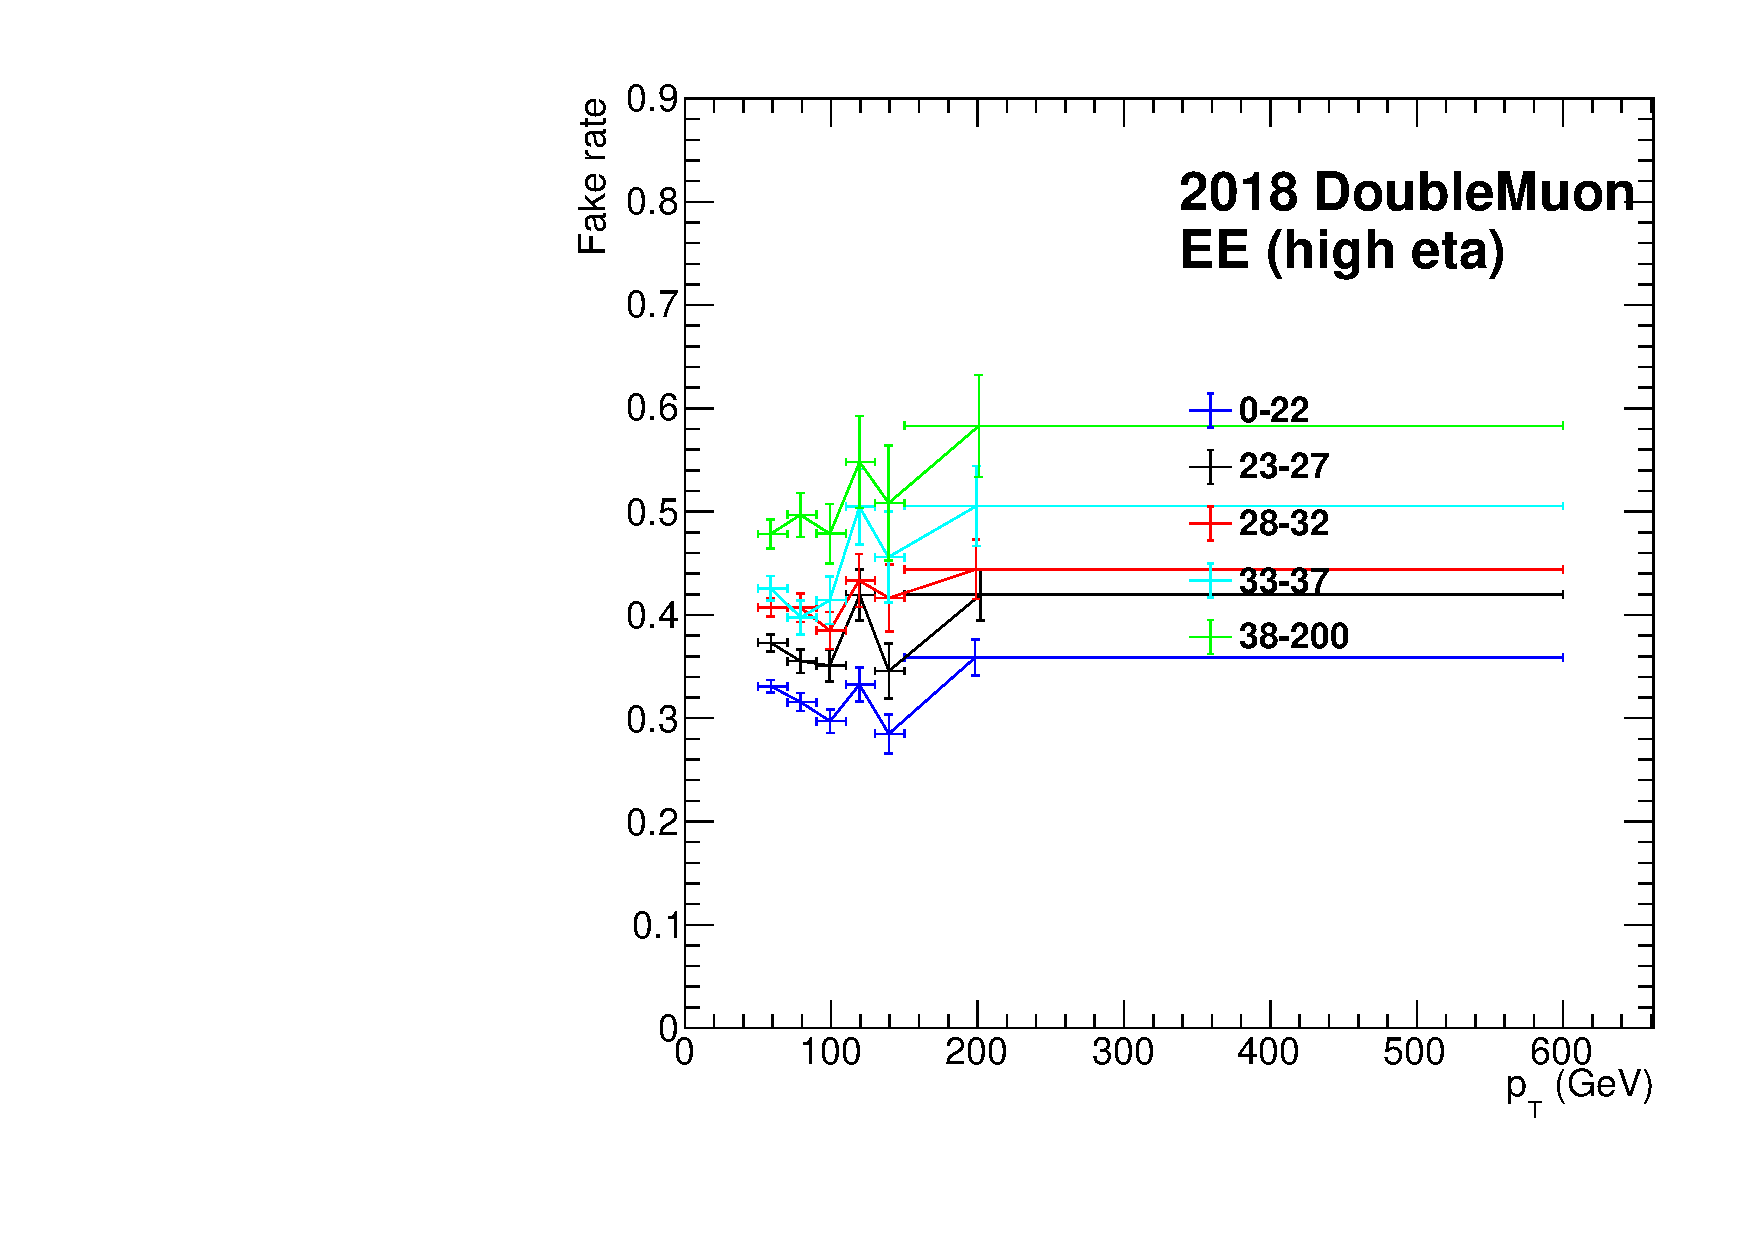
\includegraphics[width=0.3\textwidth]{fig/compare_pv_EE2_2018_doublemuon.pdf}
\label{fig:frpileup_EE2}
\end{figure}

\subsection{Fake Rate Systematics}
%% Data Sets and q/g dependence

Quarks and gluons hadronize differently. Gluon jets in general contain a larger number of particles and are therefore less likely to pass the isolation criteria of the photon ID. They therfore have a lower probability of faking a photon than quark jets. While taggers exist in data, it is difficult to distinguish between quark and gluon jets in data in an unbiased way. This represents a source of systematic uncertainty on our fake background estimation. The use of the \texttt{JetHT} and the \texttt{DoubleMuon} data sets are motivated by the need to  estimate the dependence between the fake rate on the ratio of quark to gluon flavor in the jets used in the fake rate measurement. The \texttt{JetHT} dataset is an admixture of both quark and gluon jets while the \texttt{DoubleMuon} dataset has a higher quark content. This higher quark content is due to the prevalence of EW bosons (V) which means there is a higher proportion of V+jet events. The difference between the fake rates extracted from these two datasets is taken as an estimate of the systematic uncertainty due to the quark/gluon flavor of jets. 

We emphasize that the \texttt{JetHT} and \texttt{DoubleMuon} are not MC samples but actual data sets. In the \texttt{JetHT} data set, all photons are matched within $\Delta R<0.6$ to the leading jet in the event - this removes any trigger bias that could arise if the fake photon is not the leading jet and therefore some other object has to fire the trigger. As much as possible we are trying to select photons that are comparable to the target sample composition, i.e. we would like our jet composition to be biased toward quark-initiated rather than gluon-initiated jets. By focusing on the photons near the leading jets, we achieve this goal. In principle, the \texttt{DoubleMuon} dataset covers this difference as explained earlier, but it is better to try to get the central value as close as possible. 

%% 2016 MC closure test confirmation of overall systematics?
\begin{table}[!htbp]
   \caption{There are three $n_{PV}$ bins for 2016. The 28-200 bin are further split into 3 additional bins for 2017 and 2018. The ranges are $0 \mathopen< n_{PV} \leq 22$ (left), $23 \leq n_{PV} \leq 27$ (center), and $28 \leq n_{PV} \leq 200$ (right). The ranges used for comparison were chosen to reflect a roughly uniform level of statistics between all ranges.}


       \centering
       \vspace{\baselineskip}
       \begin{tabular}{lc}
       \hline \hline
       2016 & 2017-2018\\
       \hline

       0-22 &  0-22 \\
       23-27 & 23-27 \\
       28-200 & 28-32 \\
       - & 33-37 \\
       - & 38-200\\

       \hline \hline
       \end{tabular}
       \label{table:nPV_bins}
% \end{longtable}
\end{table}

%%FIXME: fake rate dependence on Njet for subleading jets?
%%FIXME: select specific triggers within JetHT, and account for prescales?

%% pileup and Nvtx binning
Multiple interactions in each proton bunch crossings also affect our estimates of the fakes. The fake rate is then sensitive to the pileup conditions in the CMS detector as shown in Figure~\ref{fig:frpileup_compare_dataset_2016}, Figure~\ref{fig:frpileup_compare_dataset_2017}, and Figure~\ref{fig:frpileup_compare_dataset_2018}. These fake rates are binned by the number of primary vertices which are summarized in Table~\ref{table:nPV_bins}.

% generated by compare_pv_bin.exe
\begin{figure}[!htbp]
\caption{A comparison of the 2016 fake rate in EB (top), EE1 ($1.566 \mathopen< |\eta| \mathclose< 2.033$)(middle), and EE2 ($2.033 \mathopen< \lvert \eta \rvert \mathclose< 2.5$)(bottom) measured as a function of the number of selected primary vertices in the event. The ranges are $0 \mathopen< n_{PV}\mathclose\leq 22$ (left), $23 \leq n_{PV} \mathclose\leq 27$ (center), and $28 \leq n_{PV}\mathclose\leq 200$ (right). The ranges used for comparison were chosen to reflect a roughly uniform level of statistics between all ranges.}
\centering
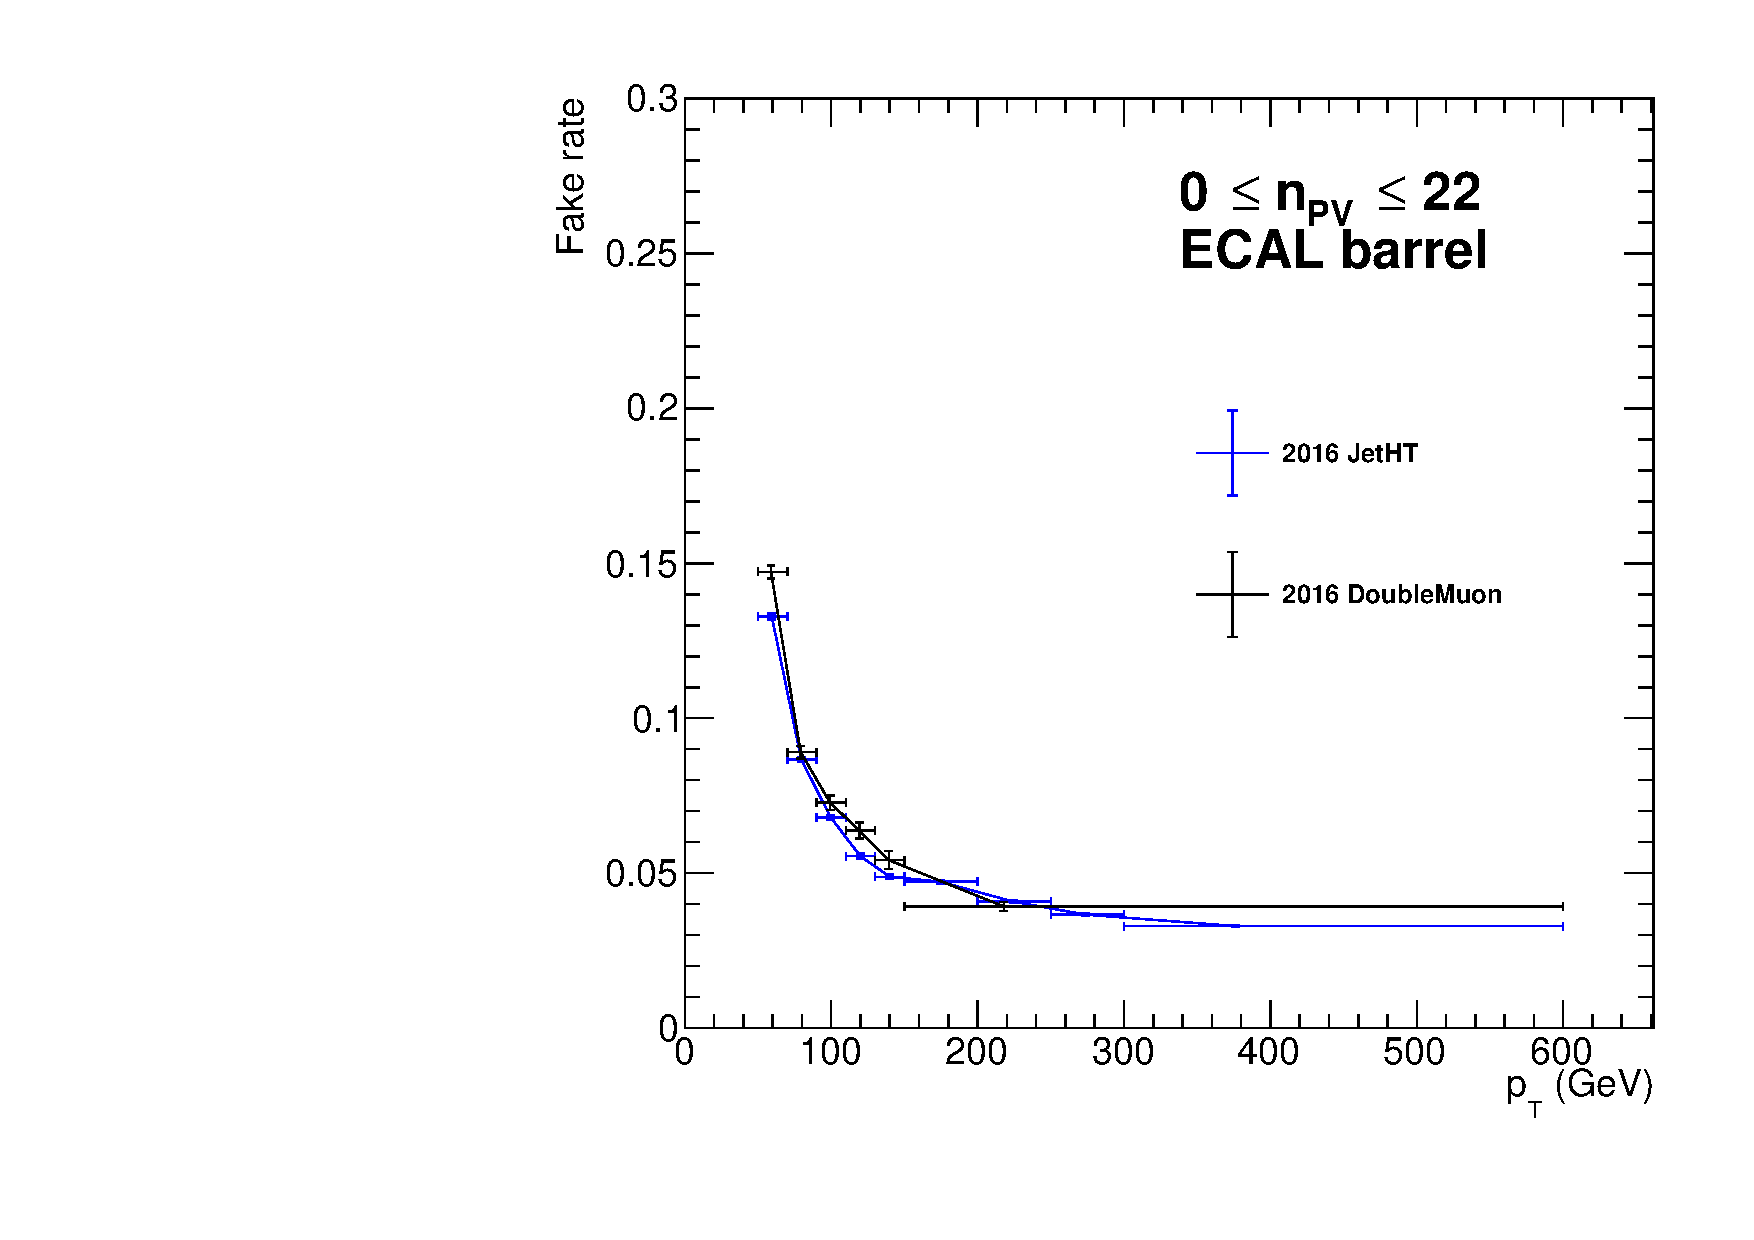
\includegraphics[width=0.3\textwidth]{fig/compare_pv_EB_2016_0to22.pdf}
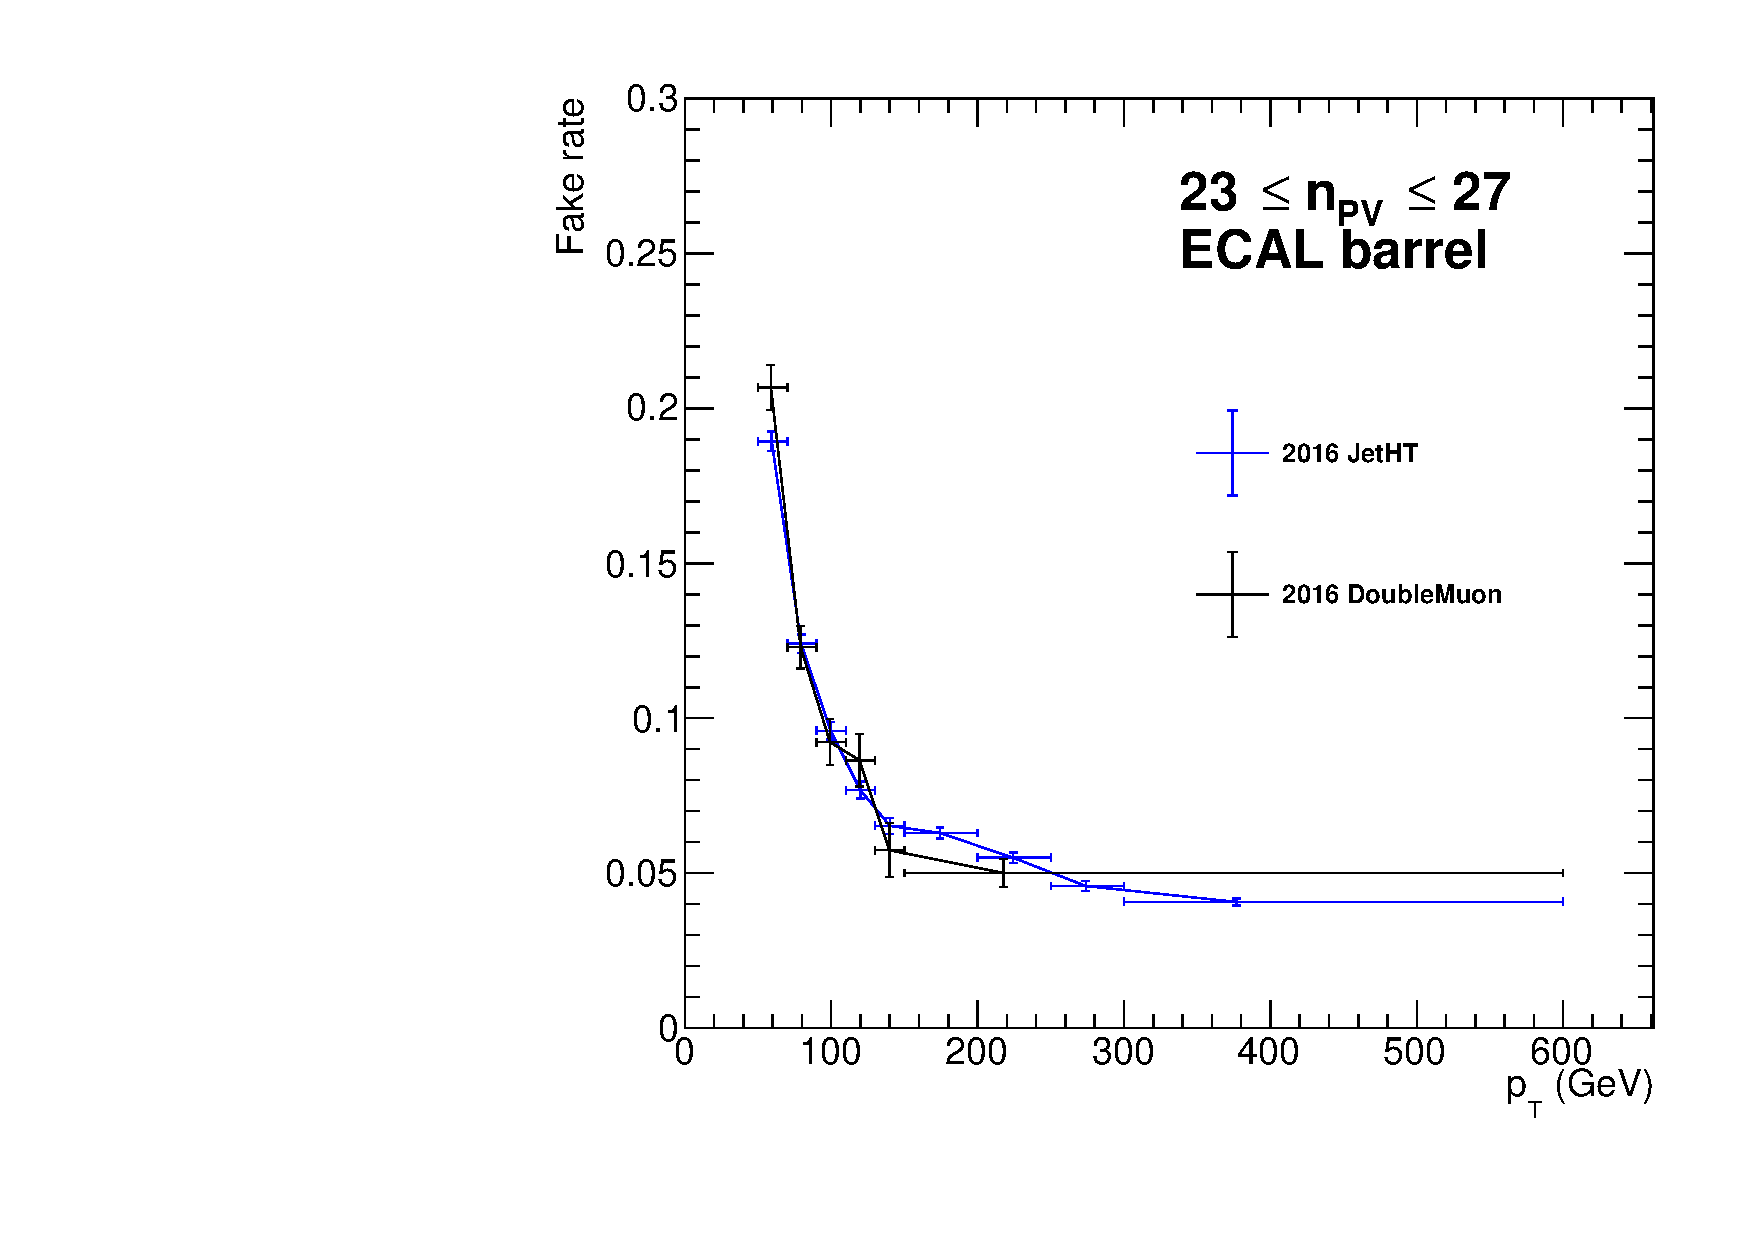
\includegraphics[width=0.3\textwidth]{fig/compare_pv_EB_2016_23to27.pdf}
\includegraphics[width=0.3\textwidth]{fig/compare_pv_EB_2016_28to200.pdf}\\
\includegraphics[width=0.3\textwidth]{fig/compare_pv_EE1_2016_0to22.pdf}
\includegraphics[width=0.3\textwidth]{fig/compare_pv_EE1_2016_23to27.pdf}
\includegraphics[width=0.3\textwidth]{fig/compare_pv_EE1_2016_28to200.pdf}\\
\includegraphics[width=0.3\textwidth]{fig/compare_pv_EE2_2016_0to22.pdf}
\includegraphics[width=0.3\textwidth]{fig/compare_pv_EE2_2016_23to27.pdf}
\includegraphics[width=0.3\textwidth]{fig/compare_pv_EE2_2016_28to200.pdf}

\label{fig:frpileup_compare_dataset_2016}
\end{figure}

% % generated by compare_pv_bin.exe
\begin{figure}[!htbp]
\caption{A comparison of the 2017 fake rate in EB (top), EE1 ($1.566 \mathopen< \mathopen| \eta \mathclose| \mathclose< 2.033$)(middle), and EE2 ($2.033 \mathopen< \mathopen| \eta \mathclose| \mathclose< 2.5$)(bottom) measured as a function of the number of selected primary vertices in the event. From left to right, the ranges are $0 \mathopen< n_{PV} \mathclose\leq 22$, $23 \leq n_{PV} \mathclose\leq 27$, $28 \leq n_{PV} \mathclose\leq 32$, $33 \leq n_{PV} \mathclose\leq 37$, and $38 \leq n_{PV} \mathclose\leq 200$. The ranges used for comparison were chosen to reflect a roughly uniform level of statistics between all ranges.}
\centering
\includegraphics[width=0.19\textwidth]{fig/compare_pv_EB_2017_0to22.pdf}
\includegraphics[width=0.19\textwidth]{fig/compare_pv_EB_2017_23to27.pdf}
\includegraphics[width=0.19\textwidth]{fig/compare_pv_EB_2017_28to32.pdf}
\includegraphics[width=0.19\textwidth]{fig/compare_pv_EB_2017_33to37.pdf}
\includegraphics[width=0.19\textwidth]{fig/compare_pv_EB_2017_38to200.pdf}\\
\includegraphics[width=0.19\textwidth]{fig/compare_pv_EE1_2017_0to22.pdf}
\includegraphics[width=0.19\textwidth]{fig/compare_pv_EE1_2017_23to27.pdf}
\includegraphics[width=0.19\textwidth]{fig/compare_pv_EE1_2017_28to32.pdf}
\includegraphics[width=0.19\textwidth]{fig/compare_pv_EE1_2017_33to37.pdf}
\includegraphics[width=0.19\textwidth]{fig/compare_pv_EE1_2017_38to200.pdf}\\
\includegraphics[width=0.19\textwidth]{fig/compare_pv_EE2_2017_0to22.pdf}
\includegraphics[width=0.19\textwidth]{fig/compare_pv_EE2_2017_23to27.pdf}
\includegraphics[width=0.19\textwidth]{fig/compare_pv_EE2_2017_28to32.pdf}
\includegraphics[width=0.19\textwidth]{fig/compare_pv_EE2_2017_33to37.pdf}
\includegraphics[width=0.19\textwidth]{fig/compare_pv_EE2_2017_38to200.pdf}
\label{fig:frpileup_compare_dataset_2017}
\end{figure}

% generated by compare_pv_bin.exe
\begin{figure}[!htbp]
\caption{A comparison of the 2018 fake rate in EB (top), EE1 ($1.566 \mathopen< |\eta| \mathclose< 2.033$)(middle), and EE2 ($2.033 \mathopen< \lvert \eta \rvert \mathclose< 2.5$)(bottom) measured as a function of the number of selected primary vertices in the event. From left to right, the ranges are $0 \mathopen< n_{PV} \mathclose\leq 22$, $23 \mathopen\leq n_{PV} \mathclose\leq 27$, $28 \mathopen\leq n_{PV} \mathclose\leq 32$, $33 \mathopen\leq n_{PV} \leq 37$, and $38 \mathopen\leq n_{PV} \mathclose\leq 200$.}

\centering
\includegraphics[width=0.19\textwidth]{fig/compare_pv_EB_2018_0to22.pdf}
\includegraphics[width=0.19\textwidth]{fig/compare_pv_EB_2018_23to27.pdf}
\includegraphics[width=0.19\textwidth]{fig/compare_pv_EB_2018_28to32.pdf}
\includegraphics[width=0.19\textwidth]{fig/compare_pv_EB_2018_33to37.pdf}
\includegraphics[width=0.19\textwidth]{fig/compare_pv_EB_2018_38to200.pdf}\\
\includegraphics[width=0.19\textwidth]{fig/compare_pv_EE1_2018_0to22.pdf}
\includegraphics[width=0.19\textwidth]{fig/compare_pv_EE1_2018_23to27.pdf}
\includegraphics[width=0.19\textwidth]{fig/compare_pv_EE1_2018_28to32.pdf}
\includegraphics[width=0.19\textwidth]{fig/compare_pv_EE1_2018_33to37.pdf}
\includegraphics[width=0.19\textwidth]{fig/compare_pv_EE1_2018_38to200.pdf}\\
\includegraphics[width=0.19\textwidth]{fig/compare_pv_EE2_2018_0to22.pdf}
\includegraphics[width=0.19\textwidth]{fig/compare_pv_EE2_2018_23to27.pdf}
\includegraphics[width=0.19\textwidth]{fig/compare_pv_EE2_2018_28to32.pdf}
\includegraphics[width=0.19\textwidth]{fig/compare_pv_EE2_2018_33to37.pdf}
\includegraphics[width=0.19\textwidth]{fig/compare_pv_EE2_2018_38to200.pdf}
\label{fig:frpileup_compare_dataset_2018}
\end{figure}

\subsection{Fake Rate Application}
The ``fake rate" obtained is used technically as a transfer function. We identify objects in the data which pass the denominator definition, then use the 'fake rate' to reweight those objects to reflect the relative probability that the object might have passed the Photon ID but is actually a jet that fragmented to look like a photon as defined by the numerator in the fake rate definition in Table~\ref{tab:fake_rate_cuts}. The data we use comes from the \texttt{DoubleEG} and \texttt{EGamma} datasets discussed in ~\label{sec:datasets}. These data sets are listed in Table~\ref{table:datasets2016-18}. We identify objects in these datasets which pass the Denominator selection in Table~\ref{tab:fake_rate_cuts} which is broadly speaking 'Loose-but-not-tight'. We call these objects Fake. There is no overlap with the 'Tight' objects, i.e. Numerator objects which pass the photon ID. Events that have an object pair where one candidate that passes the Denominator definition ('Fake') or Loose, and another candidate passes the actual photon ID (called 'Tight') are categorized as Tight-Fake (TF) or Fake-Tight (FT) depending on which object has a higher \pt. Events with objects that pass the Denominator definition are called Fake-Fake (FF). For these categories, we reweight the pair based on evaluating the appropriate fake rate function\footnote{The code for application of the fake rate is found in this \href{https://github.com/cms-exotica-diphotons/diphoton-analysis/blob/51de0227dce50e5ff11c2e0f718ca692094ee9bc/Tools/interface/fakePrediction.C#L249-L255}{link}.} depending on the eta region (EB central, EE forward, etc), pileup, and \pt of the Fake object(s). 

There are then two sources of fake background events. These are the $jj$ and $\gamma + j$, which are two jets and a photon+jet backgrounds. The $jj$ and $\gammaj$  backgrounds are estimated by reweighting each of the two $F$ objects in the data sample and by reweighting the $TF$ and $FT$ samples minus twice the $FF$ samples, respectively. This is succintly expressed as,

\begin{equation} \label{eq:nfake}
\begin{align}
   N_{jj} &= N_{LL}f_1f_2, \\
   N_{\gamma\textnormal{j}} &= N_{LT}f -  2N_{LL}f_1f_2. 
\end{align}
\end{equation}

% \begin{equation} \label{eq:jj_fakeRateApplication}
%     jj = (f_1F_1)(f_2F_2)
% \end{equation}
% where $f_i$ is the fake rate function $f$ evaluated at the \pt, $\eta$ region of photon $i=[1,2]$ and pileup. The $\gammaj$ background is a little more complicated as the $T$ objects are comprised of both real and fake photons. The $\gamma j$ background is estimated by reweighting the $TF$ and $FT$ samples minus twice the $FF$ samples as shown in Eq.~\ref{eq:gj_fakeRateApplication}. 

% \begin{equation} \label{eq:gj_fakeRateApplication}
%     \gamma j =  T_1(f_2F_2) + (f_1F_1)T_2 - 2(f_1F_1)(f_2F_2)
% \end{equation}

More details on the mathematical derivation of Eqs.~\ref{eq:nfake} is shown in Appendix~\ref{ch:appendix_fake_rate_app}. It is important to note that the $\texttt{jj}$ contribution was 100 times smaller than the $\texttt{gj}$ contribution and hence was dropped in the final limits calculation. 

\section{Photon Fake Rate Closure Test}\label{sec:closure_test}
We validated the fake rate method using an MC-based approach. The general idea is that if we apply the same method to MC, by treating it as if it were data, the results would yield a fake prediction comparable to the results from MC truth information. The MC samples that were treated as data were QCD dijets and GJets listed in Tables~\ref{table:dset-2016-closuretest} and \ref{table:dset-2017-18-closuretest}. These were chosen such that there is a sufficient number of fake photons present. The truth information on the actual number of fakes in the MC sample is obtained by matching each \texttt{pat::Photon} that passed our ID to the best final state (status 1) gen particle within $\Delta R \leq 0.1$ in the pruned collection of generated particles, if possible. In this section, we refer to photons that have been reconstructed and identified by the Particle Flow algorithm as \texttt{pat::Photon}s. If the \texttt{pat::Photon} is matched to a hadron or when the final state gen photon's comes from a hadron then they are fakes. A complication arises when the photon has multiple mothers, which is the usual case. The sole mother is chosen by finding the best match in $\Delta R$ among all of its mothers. In summary, fake photons are tagged as such if they come from hadron decays. Comparing the fake prediction from the fake rate method and using a simple counting method from the truth information, we validate our fake rate.

 The closure test has three steps. First we determine the accuracy of the fake templates produced using the sideband definition (treating MC as data) and comparing them with the MC truth templates as in Figure~\ref{fig:template_comparisons}. Second, we perform a fitting procedure where we extract the fake yields and compare with the actual yields from the MC truth information as a function of $\pt$ and $\eta$. Third, we use the fake rates from the previous step to reweight denominator objects, or objects that pass a looser photon ID, to predict the kinematics of the actual known fakes. These three steps are sequentially described in more detail below. Here we show that by splitting the EB and EE regions into inner and outer regions, the fake prediction improves as the fake rate is no longer averaged over the entire barrel or endcap region.

   % the fake rate was averaged over the entire barrel or endcap region, 


\subsection{Testing the Fake Template from the Sideband Definition}

The first step of the closure test is to create fake and real templates and validate the that the chosen sideband-defined template does a reasonable job of replicating the truth template for known fakes. The MC fake templates are filled from the MC sample listed in Tables~\ref{table:dset-2016-closuretest} and \ref{table:dset-2017-18-closuretest}, using the same selection and sideband definitions as done with the data (see Table~\ref{table:datasets2016-18}).  These templates are $\pt$-dependent so we prepared templates for $\pt$ bins of 50--70, 70--90, 90--110, 110--130, 130--150, 150--200, 200--250, 250--300, 250--300, 300--600 $\GeV$. We use coarser binning compared to the actual fake rate method due to the limited statistics in the MC samples.

In Figure~\ref{fig:template_comparisons}, we see that the fake templates for each sideband $\chiso$ choice does a reasonable job of replicating the MC truth templates. The comparison is shown for the lowest $\pt$ bin separated in EB and EE. We see that the templates don't fully replicate the MC truth because of some bias. This bias is unavoidable because fakes in a sideband are intrinsically different from fakes that pass the ID. This biasing is because of the correlation of the $\chiso$ variable with $\sieie$. This bias is the main source of systematic uncertainty on this fake rate method.

% The rest of the $\pt$ bins are found in Appendix~\ref{sec:appendix_closure_test}

The least bias is seen for the $5 < \chiso < 10$ $\GeV$ sideband making it our nominal sideband choice for the analysis.

% %%%%%%%%%%
% %
% % Closure Test Pt-binned fake rates only
% %
% %%%%%%%%%%

%%%% Template Comparisons
\begin{figure}[!htbp]
 \caption{Representative \sieie templates for the ECAL barrel (left) and endcap (right) for 2017 in the 50-70~\GeV \pt-bin are shown here. The distributions in gold show the MC truth while the black and red show the fake templates in the $5 \mathopen< \chiso \mathclose< 10$ $\GeV$ and $10 \mathopen< \chiso \mathclose< 15$ $\GeV$ sidebands.}
  \centering
  \includegraphics[width=0.49\textwidth]{fig/MCtemplates_pT50To70EB2017.pdf}
  \includegraphics[width=0.49\textwidth]{fig/MCtemplates_pT50To70EE2017.pdf}
  \label{fig:template_comparisons}
\end{figure}

\subsection{Testing the Template Fit Method for Extracting Fake Yields}

After preparing and validating the fake templates in the previous step, we fit these templates together with the real templates (same as selection as the data) to the numerator $\sieie$ distribution. Figure~\ref{fig:templatefit_closure} illustrates the fit for \pt bin $90 < \pt < 130$ $\GeV$. The numerator templates are filled with objects that pass the photon ID and it contains both real and fake photons. The real and fake templates are fitted to the numerator templates which are by definition contains both real and fake photons that pass the photon ID. In this step we extract the fake yields by fitting the fake templates prepared and validated in the previous step.

% The remaining \pt bins are shown in Appendix~\ref{sec:appendix_closure_test} \FIXME{Add the closure test appendix?}.

The template fit in $\sieie$ is performed using a negative log-likelihood function with Barlow-Beeston errors~\cite{BarlowBeeston:1993}. The fits are done for each $\pt$ bin in EB, EE and then we split the EB and EE into inner and outer regions to fine-tune the fake yield prediction. After the fit, the $\sieie$ ID cut is applied yielding a fake prediction for each separate $\pt$ bin. We then divide this fake prediction by the denominator in the MC sample, where we then get an MC fake rate as a function of $\pt$. This same procedure was repeated using two different $\chiso$ sideband choices for the MC fake templates. We then compare the obtained MC fake rate to the MC truth fake rate which was obtained by simply counting the number of fake photons in each $\pt$ bin and dividing by the denominator to get an MC truth fake rate.

We see from Figure~\ref{fig:templates_2017_etaBinnedEB} and Figure~\ref{fig:templates_2017_etaBinnedEE} a generally good agreement between the MC Truth fake rates and the MC fake rates. The "non-closure" or the failure to fully replicate the truth MC fake rates is attributed to the bias in the fake templates constructed from the sideband definition. The underprediction is minimized by choosing the sideband that is close as possible to the ID region ($\chiso < 5$ $GeV$).

In general, we observe an underprediction within an uncertainty of about 30\% as shown in Figs.~\ref{fig:fakerates_2017} and ~\ref{fig:fakerates_2018}. Note that we see larger statistical fluctuations at higher \pt due to the lack of statistics for fake photons.

% %%%%  Template Fit
\begin{figure}[!htbp]
\caption{A representative template fit from the 2018 shows using photon objects from the ECAL barrel that have \pT from 50 to 70 GeV in the \chiso sideband $5 \mathopen< \text{GeV} < 10$.}
\centering
\includegraphics[scale=0.83]{fig/fakeRatePlot_all_2017_EB_pT50To70_chIso5To10.pdf}
\label{fig:templatefit_closure}
\end{figure}

% %%%%% Fake Rates
\begin{figure}[!htbp]
 \caption{The 2017 MC Truth fake rates and the MC fake rates shows a generally good agreement with each other for both EB and EE. The MC Truth was obtained by a 'counting' procedure whereas the fake rate was obtained through a series of steps which involves a template fitting.}
  \centering
  \includegraphics[width=0.49\textwidth]{fig/closureTest_MCTruth_comparisonsEB_2017_adjustrange.pdf}
  \includegraphics[width=0.49\textwidth]{fig/closureTest_MCTruth_comparisonsEE_2017_adjustrange.pdf}
  \label{fig:fakerates_2017}
\end{figure}



\begin{figure}[!htbp]
 \caption{The 2018 MC Truth fake rates and the MC fake rates shows a generally good agreement with each other for both EB and EE. The MC Truth was obtained by a 'counting' procedure whereas the fake rate was obtained through a series of steps which involves a template fitting.}
  \centering
  \includegraphics[width=0.49\textwidth]{fig/closureTest_MCTruth_comparisonsEB_2018_adjustrange.pdf}
  \includegraphics[width=0.49\textwidth]{fig/closureTest_MCTruth_comparisonsEE_2018_adjustrange.pdf}
  \label{fig:fakerates_2018}
\end{figure}

\subsection{Testing that Reweighted Denominator Objects Reflect the Kinematics of Known Fake Objects}

The final step in the MC closure test is to verify that we can reproduce an accurate representation of the actual fake background estimate used in the analysis. We do this by reweighting the denominator objects ('photon-like' jets) with the fake rate as a function of $\pt$ for different eta regions (EB or EE). This gives us the kinematic distributions of known fake events as seen in Figure~\ref{fig:kinematics17} and Figure~\ref{fig:kinematics18}. The fake rate used to reweight the denominator distributions were obtained by fitting separate functions to the MC fake rates using the sideband choice that reflects the best ``closure" or agreement with the truth. This is the nominal sideband choice which is $5 < \chiso < 10$ $\GeV$.

Figure~\ref{fig:kinematics17} and Figure~\ref{fig:kinematics18} shows single photon kinematics for $\pt$, $\eta$, and $\phi$ for the reweighted object compared against the distributions. Agreement in the barrel is excellent but in the endcap, we see some disagreement that indicates that endcap fake rate has more eta-dependence. To verify this we split the barrel and endcap regions into inner and outer regions and went through steps 1 to 3 of the closure test. The inner barrel (EB1) corresponds to $|\eta| <  0.7221$. The outer barrel (EB2) corresponds to $0.7221 < |\eta| < 1.4442$. The inner endcap (EE1) $1.566 < |\eta| < 2.033$ while the outer endcap corresponds to $2.033 < \lvert \eta \rvert< 2.5$. We can see from the figure~\ref{fig:EtaBinned} some improvement in the agreement in the fake prediction and the MC truth fakes.

% The fake rate reweighting of the denominator objects shows an excellent agreement in the number of events in the barrel region. The endcap region fake rates suggest a finer binning of the $\eta$ range might pull the agreement between the fake prediction and the MC truth.

% % FIXME: the first time the denominator is mentioned put a footnote on photon-like jets)

% %%%%  Kinematics

% \begin{figure}[!htbp]
% \centering
% \includegraphics[width=0.45\textwidth]{fig/closure_test_photon_kinematics_eta_2017sans_Denom.pdf}
% \includegraphics[width=0.45\textwidth]{fig/closure_test_photon_kinematics_eta_2018sans_Denom.pdf}\\
% \includegraphics[width=0.45\textwidth]{fig/closure_test_photon_kinematics_phi_2017sans_Denom.pdf}
% \includegraphics[width=0.45\textwidth]{fig/closure_test_photon_kinematics_phi_2018sans_Denom.pdf} \\
% \includegraphics[width=0.45\textwidth]{fig/closure_test_photon_kinematics_pt_2017.pdf}
% \includegraphics[width=0.45\textwidth]{fig/closure_test_photon_kinematics_pt_2018.pdf}
% \caption{The two columns from the left (right) of figures show the 2017(2018) EB and EE single photon kinematic plots for reweighted objects. This final step of the closure test. The fake rate reweighting of the denominator objects shows an excellent agreement in the barrel region. The endcap region fake rates suggests a finer binning of the $\eta$ range might pull the agreement between the fake prediction and the MC truth.}
% \label{fig:kinematics}
% \end{figure}

\begin{figure}[!htbp]
\caption{The two columns show the EB (left) and EE (right) single photon kinematic plots for reweighted objects for 2017.}
\centering
\includegraphics[width=0.85\textwidth]{fig/closure_test_photon_kinematics_eta_2017sans_Denom.pdf}\\
% \includegraphics[width=0.45\textwidth]{fig/closure_test_photon_kinematics_eta_2018sans_Denom.pdf}\\
\includegraphics[width=0.85\textwidth]{fig/closure_test_photon_kinematics_phi_2017sans_Denom.pdf}\\
% \includegraphics[width=0.45\textwidth]{fig/closure_test_photon_kinematics_phi_2018sans_Denom.pdf} \\
\includegraphics[width=0.85\textwidth]{fig/closure_test_photon_kinematics_pt_2017.pdf}
% \includegraphics[width=0.45\textwidth]{fig/closure_test_photon_kinematics_pt_2018.pdf}
\label{fig:kinematics17}
\end{figure}


% \begin{figure}[!htbp]
% \centering
% \includegraphics[width=0.9\textwidth]{fig/closure_test_photon_kinematics_eta_2017sans_Denom.pdf}\\
% % \includegraphics[width=0.45\textwidth]{fig/closure_test_photon_kinematics_eta_2018sans_Denom.pdf}\\
% \includegraphics[width=0.9\textwidth]{fig/closure_test_photon_kinematics_phi_2017sans_Denom.pdf}\\
% % \includegraphics[width=0.45\textwidth]{fig/closure_test_photon_kinematics_phi_2018sans_Denom.pdf} \\
% \includegraphics[width=0.9\textwidth]{fig/closure_test_photon_kinematics_pt_2017.pdf}
% % \includegraphics[width=0.45\textwidth]{fig/closure_test_photon_kinematics_pt_2018.pdf}
% \caption{The two columns show the EB (left) and EE (right) single photon kinematic plots for reweighted objects for 2017. The fake rate reweighting of the denominator objects shows an excellent agreement in the number of events in the barrel region. The endcap region fake rates suggests a finer binning of the $\eta$ range might pull the agreement between the fake prediction and the MC truth.}
% \label{fig:kinematics17}
% \end{figure}

% \begin{figure}[!htbp]
%     \centering
%     \includegraphics[width=0.45\textwidth]{fig/closure_test_photon_kinematics_eta_2017sans_Denom.pdf}\\
%     % \includegraphics[width=0.45\textwidth]{fig/closure_test_photon_kinematics_eta_2018sans_Denom.pdf}\\
%     \includegraphics[width=0.45\textwidth]{fig/closure_test_photon_kinematics_phi_2017sans_Denom.pdf}\\
%     % \includegraphics[width=0.45\textwidth]{fig/closure_test_photon_kinematics_phi_2018sans_Denom.pdf} \\
%     \includegraphics[width=0.45\textwidth]{fig/closure_test_photon_kinematics_pt_2017.pdf}
%     % \includegraphics[width=0.45\textwidth]{fig/closure_test_photon_kinematics_pt_2018.pdf}
%     \caption{The two columns show the EB (left) and EE (right) single photon kinematic plots for reweighted objects for 2017. The fake rate reweighting of the denominator objects shows an excellent agreement in the number of events in the barrel region. The endcap region fake rates suggest a finer binning of the $\eta$ range might pull the agreement between the fake prediction and the MC truth.}
%     \label{fig:kinematics17}
% \end{figure}



\begin{figure}[!htbp]
\caption{The two columns show the EB (left) and EE (right) single photon kinematic plots for reweighted objects for 2018.}
\centering
% \includegraphics[width=0.9\textwidth]{fig/closure_test_photon_kinematics_eta_2017sans_Denom.pdf}\\
\includegraphics[width=0.9\textwidth]{fig/closure_test_photon_kinematics_eta_2018sans_Denom.pdf}\\
% \includegraphics[width=0.9\textwidth]{fig/closure_test_photon_kinematics_phi_2017sans_Denom.pdf}\\
\includegraphics[width=0.9\textwidth]{fig/closure_test_photon_kinematics_phi_2018sans_Denom.pdf} \\
% \includegraphics[width=0.9\textwidth]{fig/closure_test_photon_kinematics_pt_2017.pdf}
\includegraphics[width=0.9\textwidth]{fig/closure_test_photon_kinematics_pt_2018.pdf}
\label{fig:kinematics18}
\end{figure}

% %%%%%%%%%%%
% %
% % Closure Test with Eta-binned Fake Rates
% %
% %%%%%%%%%%

% %%%%  Template Fit

% %
\begin{figure}[!htbp]
\caption{A representative template fit from the 2017.}
\centering
\includegraphics[scale=0.85]{fig/fakeRatePlot_all_2017_EB1_pT50To70_chIso5To10.pdf}
\label{fig:templatefit_2017_etabinned}
\end{figure}

% %%%%% Fake Rates
\begin{figure}[!htbp]
  \caption{The Fake Rates were recalculated with the splitting of the barrel region into inner and outer regions. The inner barrel (EB1) corresponds to $|\eta| <  0.7221$. The outer barrel (EB2) corresponds to $0.7221 < |\eta| < 1.4442$. This was done to improve the agreement between the fake prediction and the MC Truth fake prediction for the last step of the closure test.}
  \centering
  \includegraphics[width=0.49\textwidth]{fig/closureTest_MCTruth_comparisonsEB1_2017_adjustrange.pdf}
  \includegraphics[width=0.49\textwidth]{fig/closureTest_MCTruth_comparisonsEB2_2017_adjustrange.pdf}
  \label{fig:templates_2017_etaBinnedEB}
\end{figure}

\begin{figure}[!htbp]
  \caption{We also split the endcaps into inner and outer regions to improve the fake prediction. The inner endcap (EE1) $1.566 < |\eta| < 2.033$ while the outer endcap corresponds to $2.033 < \lvert \eta \rvert< 2.5$.}
  \centering
  \includegraphics[width=0.49\textwidth]{fig/closureTest_MCTruth_comparisonsEE1_2017_adjustrange.pdf}
  \includegraphics[width=0.49\textwidth]{fig/closureTest_MCTruth_comparisonsEE2_2017_adjustrange.pdf}
  % \includegraphics[width=0.3\textwidth]{fig/closureTest_MCTruth_comparisonsEE3_2017_adjustrange.pdf}
  \label{fig:templates_2017_etaBinnedEE}
\end{figure}

% %%%%  Kinematics

\begin{figure}[!htbp]
\centering
\caption{Splitting the barrel and endcap regions shows some improvements in the agreement between the fake rate reweighted Fake Prediction and the MC Truth Prediction for 2017. A similar result is observed for 2018. The inner barrel (EB1) corresponds to $|\eta| < 0.7221$. The outer barrel (EB2) corresponds to $0.7221 < |\eta| < 1.4442$. The inner endcap (EE1) $1.566 < |\eta| < 2.033$ while the outer endcap corresponds to $2.033 < |\eta| < 2.5$.}
\includegraphics[width=0.8\textwidth]{fig/closure_test_photon_kinematics_eta_2017_withEtaBin.pdf}\\
\includegraphics[width=0.8\textwidth]{fig/closure_test_photon_kinematics_phi_2017_withEtaBin.pdf}\\
\includegraphics[width=0.8\textwidth]{fig/closure_test_photon_kinematics_pt_2017_withEtaBin.pdf}
\label{fig:EtaBinned}
\end{figure}

\subsection{Conclusions from the Closure Test}

The fake rate method was validated via the Closure Test by applying the same steps on MC. The fake rate extracted from the method does a reasonable job of replicating the MC Truth fake rate as shown in Figure~\ref{fig:fakerates_2017} and ~\ref{fig:fakerates_2018}. Approximately 30\% non-closure across the $0-600$ GeV pT range was observed. It was also observed that splitting the endcap and barrel into inner and outer regions improved the agreement between the kinematic plots of the Fake Prediction and the MC Truth. The inner barrel (EB1) corresponds to $|\eta| <  0.7221$. The outer barrel (EB2) corresponds to $0.7221 < |\eta| < 1.4442$. The inner endcap (EE1) $1.566 < |\eta| < 2.033$ while the outer endcap corresponds to $2.033 < \lvert \eta \rvert< 2.5$. In principle, implementing a further finer binning strategy would likely enhance the agreement between between the MC truth and the Fake prediction but it cocmes at the cost of reduced statistical reliability within individual bins.

% =CLOSURE ======================================================================
% he γj background estimation takes more care because the T objects are comprised of real photons (R) and not real photons (N), i.e., T = R + N, where N = fF. The γj background is estimated over all data events according to:

% =======================================================================

% \begin{equation}
%     P(T|\gamma) = \frac{f}{1+f}
% \end{equation}


% If an event has an object pair where both objects pass the Denominator definition, we call this Fake-Fake. For these categories, we then reweight the pair based on evaluating the appropriate fake rate function depending on the eta region (EB central, EE forward, etc), pileup, and pT of the Fake object(s). This reweighting applies only to the event weight. If say the fake rate factor is evaluated to 0.3 for a certain object, this means in a sense that the current object pair is expected to contribute 0.3 events to the fake contribution in the ‘signal’ selection. The kinematics (\pt, \eta, $M_{gg}$, etc) are not changed, only the overall weight.

% For Fake-Fake pairs, the reweight factor is calculated as the product of the two weights for the individual objects. This procedure gives the predicted contribution of fake photons from jets to the ‘signal’ selection of two candidates passing our Photon ID (called Tight-Tight).

% The


% ======================================================================================

%%Beam halo in fake rate - bump in sieie tail at high pt? See pg 29 of AN-17-030

%%sideband variation

%%flipping the sideband/template variables?





% generated by efficiency.exe
% \FIXME{NEED to redo the TF Photon Efficiency}
% \begin{figure}[tbp!]
% \begin{center}
% \includegraphics[angle=0,width=0.3\textwidth]{fig/eff_2016_TFPhoton2_pt_fake.pdf}
% \includegraphics[angle=0,width=0.3\textwidth]{fig/eff_2017_TFPhoton2_pt_fake.pdf}
% \includegraphics[angle=0,width=0.3\textwidth]{fig/eff_2018_TFPhoton2_pt_fake.pdf}
% \end{center}
% \caption{Efficiency of \texttt{HLT\_DoublePhoton60} (2016) or \texttt{HLT\_DoublePhoton70} (2017-2018) trigger (measured with reference trigger the logical \texttt{OR} of all \texttt{HLT\_PFJetXYZ}) as a function of the \pt of the second-leading photon numerator candidates in 2016 (left), 2017 (center) and 2018 (right) data.}
% \label{fig:trigger_efficiency_fake}
% \end{figure}

\clearpage


% After the fake rate is calculated, it is applied as a weight to each fake candidate in the \texttt{DoubleEG/EGamma} data sets, as a function of the \pt and region (EB or EE) of the candidate.
% The prediction of true-fake, fake-true and fake-fake contributions to the \mgg distribution are shown in Figure~\ref{fig:fake_comparison_BB} and Figure~\ref{fig:fake_comparison_BE} for the barrel-barrel and barrel-endcap regions, respectively. For the purpose of showing the differences among the predictions, these predictions are scaled to an integrated luminosity of 1\fbinv.
% {\em Be aware that the 2017 and 2018 predictions are scaled down by an addition factor of 2.}
% The additional factor of two difference between the 2016 and the 2017-2018 fake rate predictions is current under study.
% However, the consistency of the factor of two discrepancy between the \texttt{DoubleMuon} and \texttt{JetHT} data sets, and the consistency of the factor of two across many kinematic variables is suggestive of a single effect in the \texttt{EGamma} dataset.

% % generated by compare_fake_predictions.exe
% \begin{figure}[tbp!]
% \begin{center}
% \includegraphics[angle=0,width=0.3\textwidth]{fig/fake_compare/compare_fake_pred_Minv_BB_jetht.pdf}}
% \includegraphics[angle=0,width=0.3\textwidth]{fig/fake_compare/compare_fake_pred_Minv_BB_average.pdf}}
% \includegraphics[angle=0,width=0.3\textwidth]{fig/fake_compare/compare_fake_pred_Minv_BB_doublemuon.pdf}}\\
% \includegraphics[angle=0,width=0.3\textwidth]{fig/fake_compare/compare_fake_pred_pt1_BB_jetht.pdf}}
% \includegraphics[angle=0,width=0.3\textwidth]{fig/fake_compare/compare_fake_pred_pt1_BB_average.pdf}}
% \includegraphics[angle=0,width=0.3\textwidth]{fig/fake_compare/compare_fake_pred_pt1_BB_doublemuon.pdf}}\\
% \includegraphics[angle=0,width=0.3\textwidth]{fig/fake_compare/compare_fake_pred_pt2_BB_jetht.pdf}}
% \includegraphics[angle=0,width=0.3\textwidth]{fig/fake_compare/compare_fake_pred_pt2_BB_average.pdf}}
% \includegraphics[angle=0,width=0.3\textwidth]{fig/fake_compare/compare_fake_pred_pt2_BB_doublemuon.pdf}}
% \end{center}
% \caption{Contributions to predicted \mgg distribution in the barrel-barrel category from fake photons, where the fake rate is calculated from the \texttt{JetHT} (left) and \texttt{DoubleMuon} (right) data sets, and the average of the two fake rates (center). The top, center and bottom plots display \mgg, $p_{T1}$, and $p_{T2}$, respectively.}
% \label{fig:fake_comparison_BB}
% \end{figure}

% \clearpage

% % generated by compare_fake_predictions.exe
% \begin{figure}[tbp!]
% \begin{center}
% \includegraphics[angle=0,width=0.3\textwidth]{fig/fake_compare/compare_fake_pred_Minv_BE_jetht.pdf}}
% \includegraphics[angle=0,width=0.3\textwidth]{fig/fake_compare/compare_fake_pred_Minv_BE_average.pdf}}
% \includegraphics[angle=0,width=0.3\textwidth]{fig/fake_compare/compare_fake_pred_Minv_BE_doublemuon.pdf}}\\
% \includegraphics[angle=0,width=0.3\textwidth]{fig/fake_compare/compare_fake_pred_pt1_BE_jetht.pdf}}
% \includegraphics[angle=0,width=0.3\textwidth]{fig/fake_compare/compare_fake_pred_pt1_BE_average.pdf}}
% \includegraphics[angle=0,width=0.3\textwidth]{fig/fake_compare/compare_fake_pred_pt1_BE_doublemuon.pdf}}\\
% \includegraphics[angle=0,width=0.3\textwidth]{fig/fake_compare/compare_fake_pred_pt2_BE_jetht.pdf}}
% \includegraphics[angle=0,width=0.3\textwidth]{fig/fake_compare/compare_fake_pred_pt2_BE_average.pdf}}
% \includegraphics[angle=0,width=0.3\textwidth]{fig/fake_compare/compare_fake_pred_pt2_BE_doublemuon.pdf}}
% \end{center}
% \caption{Contributions to predicted \mgg distribution in the barrel-endcap category from fake photons, where the fake rate is calculated from the \texttt{JetHT} (left) and \texttt{DoubleMuon} (right) data sets, and the average of the two fake rates (center). The top, center and bottom plots display \mgg, $p_{T1}$, and $p_{T2}$, respectively.}
% \label{fig:fake_comparison_BE}
% \end{figure}

\clearpage




\newpage
% \section{References}
% \renewcommand{\bibsection}{}%removes the spaces and unwanted references heading from the list
% \begin{singlespacing}
% \bibliographystyle{apsrev}
% \bibliography{Ref_Background.bib}
% \end{singlespacing}\par
% %{\let\thefootnote\relax\footnote{{Copyright: \copyright 2019 Elsevier B.V.}}}




%Feynman Diagrams must compile with LuaLatex to render properly
%%% Some minimal working examples below
% \feynmandiagram [horizontal=a to b] {
%   i1 [particle=\(e^{-}\)] -- [fermion, very thick] a -- [fermion, opacity=0.2] i2 [particle=\(e^{+}\)],
%   a -- [red, photon, edge label=\(\gamma\), momentum'={[arrow style=red]\(k\)}] b,
%   f1 [particle=\(\mu^{+}\)] -- [fermion, opacity=0.2] b -- [fermion, very thick] f2 [particle=\(\mu^{-}\)],
% };

% \feynmandiagram [horizontal=a to b] {
%   i1 -- [fermion] a -- [fermion] i2,
%   a -- [photon] b,
%   f1 -- [fermion] b -- [fermion] f2,
% };

% \feynmandiagram [small, horizontal=a to t1] {
%   %a [particle=\(\pi^{0}\)] -- [scalar] t1 -- t2 -- t3 -- t1,
%   a [particle=\(\gluon\)] -- [scalar] t1 -- t2 -- t3 -- t1,
%   t2 -- [photon] p1 [particle=\(\gamma\)],
%   t3 -- [photon] p2 [particle=\(\gamma\)],
%   p1 -- [opacity=0.2] p2,
% };

% \begin{tikzpicture}
%   \begin{feynman}
%     \vertex (a) {\(\mu^{-}\)};
%     \vertex [right=of a] (b);
%     \vertex [above right=of b] (f1) {\(\nu_{\mu}\)};
%     \vertex [below right=of b] (c);
%     \vertex [above right=of c] (f2) {\(\overline \nu_{e}\)};
%     \vertex [below right=of c] (f3) {\(e^{-}\)};

%     \diagram* {
%       (a) -- [fermion] (b) -- [fermion] (f1),
%       (b) -- [boson, edge label'=\(W^{-}\)] (c),
%       (c) -- [anti fermion] (f2),
%       (c) -- [fermion] (f3),
%     };
%   \end{feynman}
% \end{tikzpicture}


